% !TeX program = lualatex
% !TeX encoding = utf8

\documentclass[aspectratio=169, 10pt]{beamer}

\usepackage{amsmath}
\usepackage[T1]{fontenc}

\usepackage{lhcb_presentation/package}

\usepackage{units}
\usepackage{graphicx}
\usepackage{booktabs}
\usepackage{ulem}
\usepackage{bm}
\usepackage{comment}
\usepackage{tikz}

\usetikzlibrary{decorations.pathreplacing}

\definecolor{brickred}{rgb}{0.85, 0, 0.05}
\errorcontextlines 10000

\title[Hybrid DL approach to vertexing]{A hybrid deep learning approach to vertexing}

\author[Fang, Schreiner, Sokoloff, Weisser, Williams]{
   Rui Fang\textcolor{red}{\inst{1}} \and
   Henry Schreiner\textcolor{red}{\inst{1, 2}} \and
   Mike Sokoloff\textcolor{red}{\inst{1}} \and
   Constantin Weisser\textcolor{red}{\inst{3}} \and
   J Michael Williams\textcolor{red}{\inst{3}}}
\institute{
    \inst{1} The University of Cincinnati \and
    \inst{2} Princeton University \and
    \inst{3} Massachusetts Institute of Technology
}
\date{March 11, 2019}

\renewcommand{\logomax}{\node [right] at (.25,1.9) {
\includegraphics[height=1.8cm]{images/acatlogo.pdf}};}
\renewcommand{\logomini}{\node at (.5,.4) {
\includegraphics[height=.75cm]{images/acatlogo.pdf}};}

\begin{document}

\begin{frame}
    \titlepage
    \begin{tikzpicture}[overlay]
        \node [below] at (0.25, -1.9) {\color{lhcbLightBlue}ACAT 2019};
        %\node [above] at (4.7, -1.9) {
\includegraphics[width=2cm]{images/acatlogo.pdf}};
        \node [above] at (6.9, -1.9) {
\includegraphics[width=4cm]{images/iris-hep-t.png}};
    \end{tikzpicture}
\end{frame}

%%%%%%%%%%%%%%%%%%%%%%%%%%%%%%%%%%%%%%%%%%%%%%%%%%%%%%%%%%%%%%%%%%%%%%%%%%%%%%%

\section{Introduction}

%Add eff plots here
\subsection{Conclusion}
\begin{frame}{Conclusion}
    \centering
    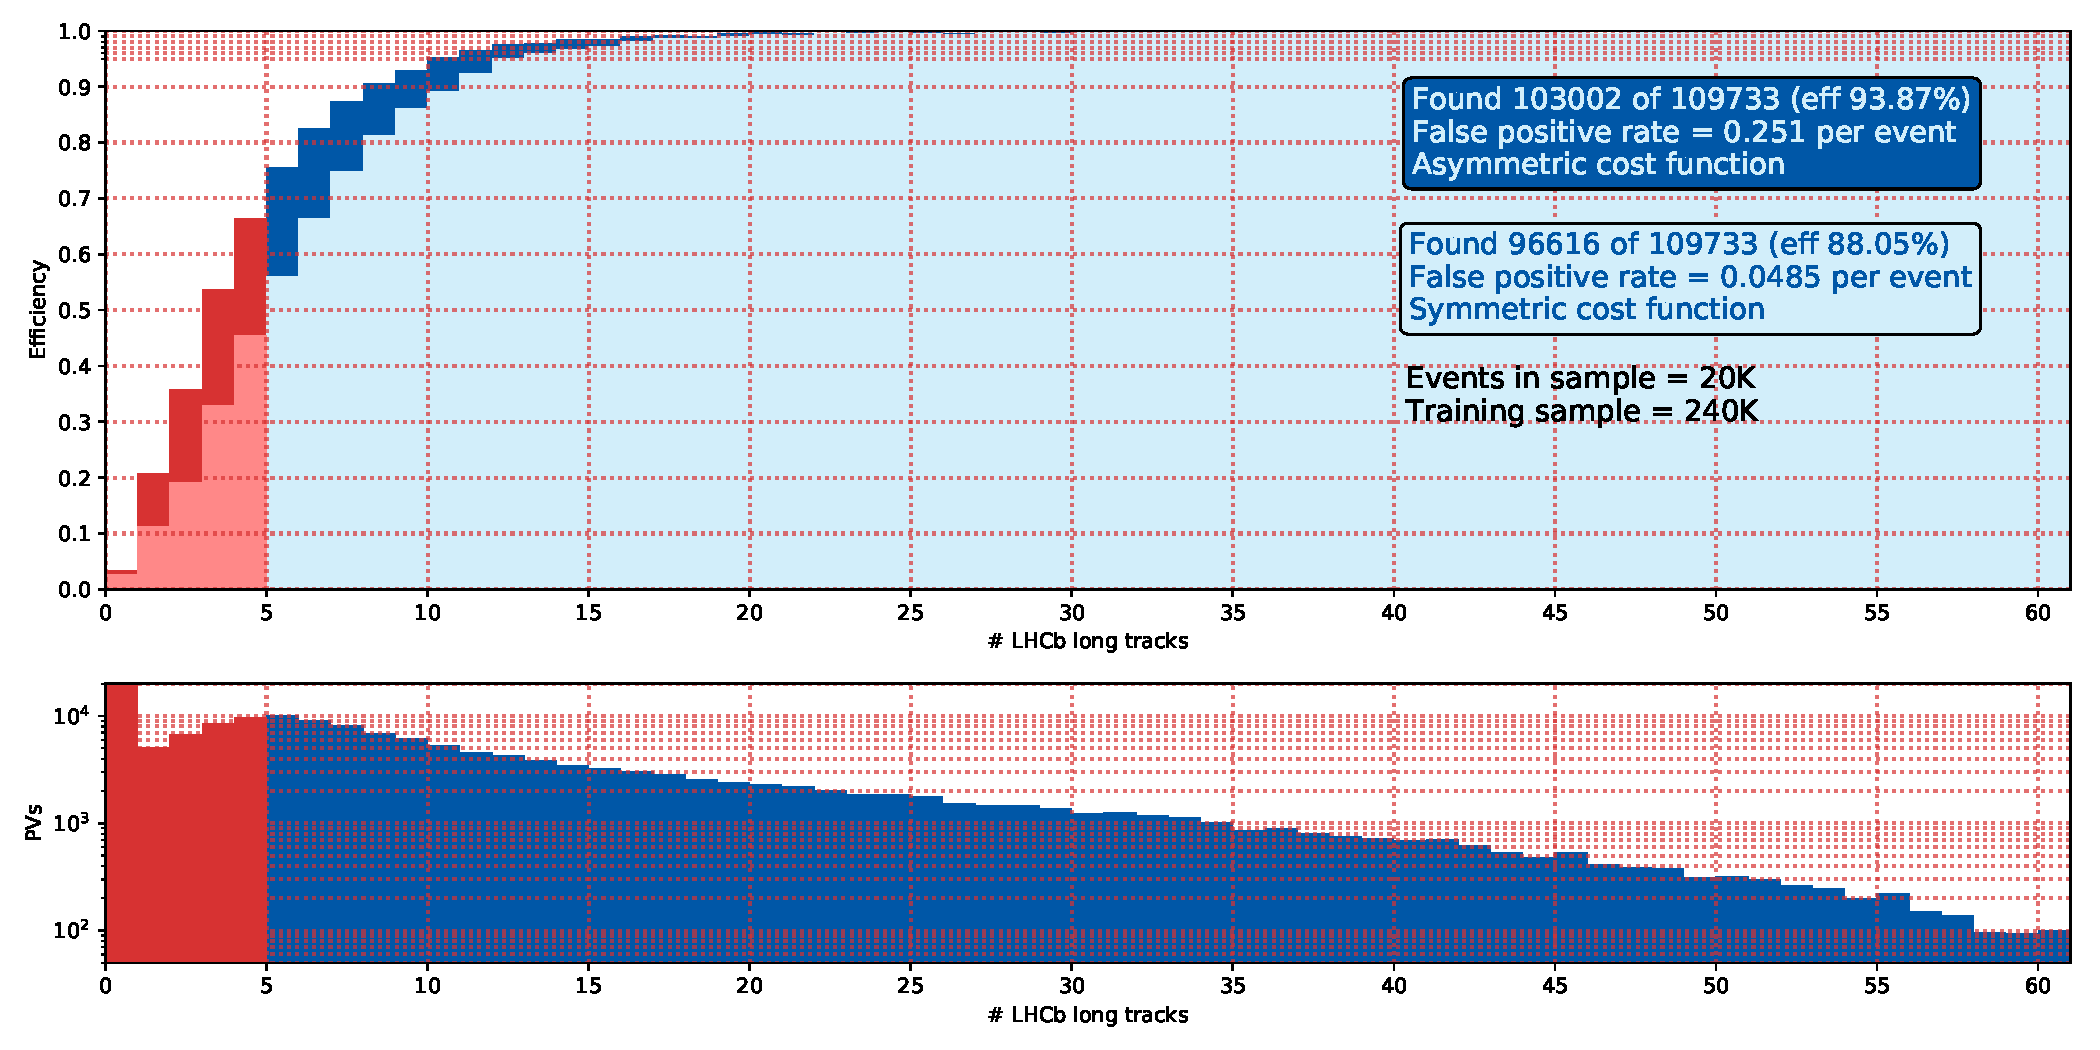
\includegraphics[width=.7\textwidth]{images/effntracks.pdf}
\end{frame}


\subsection{Tracking in the LHCb upgrade}
\begin{frame}{Tracking in the LHCb upgrade}
  \begin{columns}[c]
    \column{.5\textwidth}
    \begin{block}{The changes}
      \begin{itemize}
          \item 30 MHz software trigger
          \item 7.6 PVs per event (Poisson distribution)
          \item Roughly 5.5 visible PVs per event
      \end{itemize}
    \end{block}
    \begin{block}{The problem}
    \begin{itemize}
    	\item Much higher pileup
    	\item Very little time to do the tracking
    	\item Current algorithms too slow
    \end{itemize}
    \end{block}
    \column{.5\textwidth}
      \begin{center}
    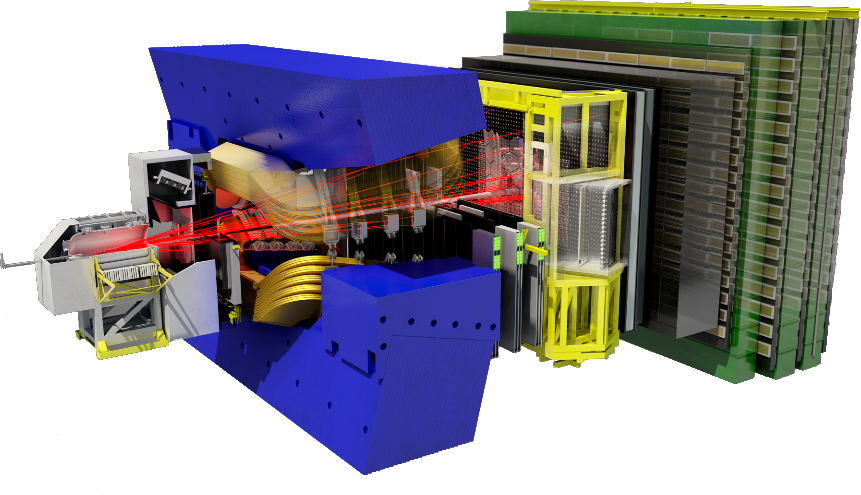
\includegraphics[width=\textwidth, trim=18 0 18 0]{images/LHCbDet.png}
  \end{center}
  \end{columns}

  \vspace{1em}
  \begin{center}
    \textbf{We need to rethink our algorithms from the ground up...}
  \end{center}
\end{frame}


\subsection{Vertices and tracks}
\begin{frame}{Vertices and tracks}
\begin{columns}[c]
    \column{.5\textwidth}
    \begin{block}{Vertices}
      \begin{itemize}
          \item Events contain $\approx 7$ Primary Vertices (PVs)
          \begin{itemize}
            \item A PV should contain 5+ long tracks
          \end{itemize}
          \item Multiple Secondary Vertices (SVs) per event as well
          \begin{itemize}
            \item A SV should contain 2+ tracks
          \end{itemize}
      \end{itemize}
    \end{block}

    \column{.5\textwidth}
    \begin{tikzpicture}
        [beam/.style={line width = 15, opacity=.1, lhcbBlue, shorten >= -.2cm, shorten <= -.2cm},
        PV/.style={lhcbRed, circle, fill, inner sep=1pt},
        SV/.style={green!70!black, circle, fill, inner sep=1pt},
        track/.style={lhcbBlue, thick}]

        \clip [use as bounding box] (-3,-2) rectangle (3,2);
        \clip (-3,-2) rectangle (3,2);

        \node [lhcbBlue!80!white, rotate=-5] at (-2, .7) {Beams};
        \draw [beam] (-3,.3) -- (3,-.3);
        \draw [beam] (-3,-.3) -- (3,.3);

        \node [PV] (A) at (1.2, -.05) {};
        \node [PV] (B) at (-.8, .15) {};
        \node [lhcbRed, above] at (B) {PV};

        \draw [track] (A) -- (3,1.3);
        \draw [track] (A) -- (3,1);
        \draw [track] (A) -- (3,.5);

        \draw [track] (B) -- (3,1.4) node [midway, above, rotate=17] {Track};
        \draw [track] (B) -- (3,.6);
        \draw [track] (B) -- (3,-.5);
        \draw [track, dashed] (B) -- (1,-.5);

        \node [SV] (C) at (1,-.5) {};
        \node [green!70!black, below] at (C) {SV};
        \draw [track] (C) -- (3, -.3);
        \draw [track] (C) -- (3, .3);
        \draw [track] (C) -- (3, -1.1);
    \end{tikzpicture}
  \end{columns}


  \begin{block}{Adapt to machine learning?}
  \begin{itemize}
      \item Sparse 3D data (41M pixels) $\to$ rich 1D data
      \item 1D convolutional neural nets
      \item Highly parallelizable, GPU friendly
      \item Opportunities to visualize learning process
  \end{itemize}
  \end{block}
\end{frame}


\subsection{A hybrid ML approach}
\begin{frame}{A hybrid ML approach}

\begin{tikzpicture}[
    scale=.95,
    belowbox/.style={fill=lhcbLightBlue},
    topbox/.style={fill=lhcbBlue},
    texttop/.style={below, lhcbLightBlue},
    track/.style={thick, lhcbBlue},
    minibox/.style={draw, thick, minimum width=.1cm, minimum height=.1cm, lhcbBlue},
    miniarr/.style={->, thick, lhcbBlue},
    conn/.style={-latex, ultra thick, lhcbBlue}
    ]
    	\begin{scope}
    	    \path [belowbox] (-1.5,-1) rectangle (1.5,.45);
    		\draw [track] (0,-.275) -- (-1.5,-.9);
    		\draw [track] (0,-.275) -- (-1.5,-.6);
    		\draw [track] (0,-.275) -- (-1.5,.2);
    		\draw [track] (0,-.275) -- (1.5,-.3);
    		\draw [track] (0,-.275) -- (1.5,-.6);
    		\draw [track] (0,-.275) -- (1.5,.85);
    		\draw [track] (0,-.275) -- (-.5,-1);
    		\draw [track] (.4, -.6) -- (1.3,-1);
    		\draw [track] (.4, -.6) -- (.7,-1);
    		\path [topbox]  (-1.5,.45) rectangle (1.5,1);
    	    \node at (0,1) [texttop] {Tracking};
            \path [fill=lhcbRed] (0, -.275) circle (.05);
            \path [fill=green!70!black] (.4, -.6) circle (.05);
    	\end{scope}

    	\begin{scope}[xshift=4cm]
    	    \path [belowbox] (-1.5,-1) rectangle (1.5,.45);
    		\path [fill=lhcbBlue] plot [smooth] coordinates {
    			(-1.5,-1)
    			(-1.1, -.98)
    			(-.9, -.9)
    			(-.5, -.6)
    			(0, .2)
    			(.2, -.2)
    			(.4, 0)
    			(.8, -.7)
    			(1.1, -.9)
    			(1.3, -.98)
    			(1.5,-1)
    		};
    		\path [topbox]  (-1.5,.45) rectangle (1.5,1);
    	    \node at (0,1) [texttop] {Kernel generation};
    	\end{scope}

    	\begin{scope}[xshift=8cm]
    	    \path [belowbox] (-1.5,-1) rectangle (1.5,.45);
    		\node [minibox] (mA) at (-1,-.3) {};
    		\node [minibox] (mB) at (-.5,-.3) {};
    		\node [minibox] (mC) at (0,-.3) {};
    		\node [minibox] (mD) at (.5,-.3) {};
    		\node [minibox] (mE) at (1,-.3) {};
    		\draw [miniarr] (mA) -- (mB);
    		\draw [miniarr] (mB) -- (mC);
    		\draw [miniarr] (mC) -- (mD);
    		\draw [miniarr] (mD) -- (mE);

    		\path [topbox]  (-1.5,.45) rectangle (1.5,1);
    	    \node at (0,1) [texttop] {CNN to find PVs};
    	\end{scope}

    	\begin{scope}[xshift=12cm]
    	    \path [belowbox] (-1.5,-1) rectangle (1.5,.45);
    		\path [fill=lhcbBlue] plot [smooth] coordinates {
    		(-.15,-1)
    		(0, 0)
    		(.15,-1)
    		};
    		\path [fill=lhcbBlue] plot [smooth] coordinates {
    		(.25,-1)
    		(.4, 0)
    		(.55,-1)
    		};
    		\path [topbox]  (-1.5,.45) rectangle (1.5,1);
    	    \node at (0,1) [texttop] {Interpret results};
    	\end{scope}

    	\begin{scope}[xshift=0cm, yshift=-2.5cm]
    	    \path [belowbox] (-1.5,-1) rectangle (1.5,.45);
    		\path [fill=lhcbRed] plot [smooth] coordinates {
    		(-.15,-1)
    		(0, 0)
    		(.15,-1)
    		};
    		\path [fill=green!70!black] plot [smooth] coordinates {
    		(.25,-1)
    		(.4, 0)
    		(.55,-1)
    		};
    		\path [topbox]  (-1.5,.45) rectangle (1.5,1);
    	    \node at (0,1) [texttop] {Truth};
    	\end{scope}

    	\draw [conn] (1.5,0) -- (2.5,0);
    	\draw [conn] (5.5,0) -- (6.5,0);
    	\draw [conn] (9.5,0) -- (10.5,0);
    	\draw [conn] (1.5, -2.5) -- (7, -1.1) node [above=-2.5, midway, rotate=13] {Training};
    	\draw [conn] (1.5, -3) -- (11, -1.1) node [above=-1, midway, rotate=11] {Validation};
\end{tikzpicture}

\begin{block}{Machine learning features (so far)}
    \begin{itemize}
        \item Prototracking converts sparse 3D dataset to feature-rich 1D dataset
        \item Easy and effective visualization due to 1D nature
        \item Even simple networks can provide interesting results
    \end{itemize}
\end{block}

\vspace{.3em}
\begin{center}
What follows is a proof of principle implementation for finding PVs.
\end{center}
\end{frame}



%%%%%%%%%%%%%%%%%%%%%%%%%%%%%%%%%%%%%%%%%%%%%%%%%%%%%%%%%%%%%%%%%%%%%%%%%%%%%%%

\section{Design}

\subsection{Kernel generation}
\begin{frame}{Kernel generation}
  \begin{columns}[c]
    \column{.54\textwidth}

        \begin{block}{Tracking procedure}
        \begin{itemize}
            \item Hits lie on the 26 planes
            \item For simplicity, only 3 tracks shown
            \uncover<2->{%
            \item Make a 3D grid of voxels (2D shown)
            \item \textcolor{lhcbRed}{Note: only $z$ will be fully calculated and stored}
            }
            \uncover<3->{%
            \item Tracking (full or partial)
            }
            \uncover<4->{%
            \item Fill in each voxel center with Gaussian PDF
            }
            \uncover<5->{%
            \item PDF for each (proto)track is combined
            }
            \uncover<6->{%
            \item Stores $z$ histogram with maximum KDE value
            }
        \end{itemize}
        \end{block}

    \column{.46\textwidth}
    \begin{tikzpicture}
        [hit/.style={inner sep=2pt, fill, circle, black!80!red},
        simitrack/.style={shorten >= -6cm, shorten <= -6cm, opacity=.2, line width=.1cm,
            preaction={draw, line width=.3cm, opacity=.2},
            preaction={draw, line width=.5cm, opacity=.2}},
        bluesimitrack/.style={thick, blue,
            preaction={shorten >= -6cm, shorten <= -6cm, draw, opacity=.2, line width=.1cm,
                preaction={draw, blue, line width=.3cm, opacity=.2},
                preaction={draw, blue, line width=.5cm, opacity=.2}}}
        ]

        \node at (2,-3) [below] {$z$ axis (along the beam)};
        \node at (-1, 0) [left] {$x$};

        \clip (-1,-3) rectangle (5,3);

        \begin{scope}[xscale=.65, xshift=-.6cm]

        % def f(name, slope, factor):
        %     v = np.arange(1,9)
        %     vv = (v-.5)*slope + .05*np.sin(v*factor)
        %     q = np.linspace(.5, 8, 400)
        %     qq = (q-.5)*slope + .05*np.sin(q*factor)
        %     print(f'% {name} slope={slope} factor={factor}')
        %     for a,b in zip(v,vv):
        %         print(f'\coordinate ({name}{a}) at ({a}, {b:.3});')
        %     print()
        %     return q, qq, v, vv


        % (v-.5)*slope + .05*np.sin(v*factor)
        % A slope=0.4 factor=-5
        \coordinate (A7) at (1, 0.248);
        \coordinate (A6) at (2, 0.627);
        \coordinate (A5) at (3, 0.967);
        \coordinate (A4) at (4, 1.35);
        \coordinate (A3) at (5, 1.81);
        \coordinate (A2) at (6, 2.25);
        \coordinate (A1) at (7, 2.62);

        % B slope=0.06 factor=6
        \coordinate (B8) at (1, 0.016);
        \coordinate (B7) at (2, 0.0632);
        \coordinate (B6) at (3, 0.112);
        \coordinate (B5) at (4, 0.165);
        \coordinate (B4) at (5, 0.221);
        \coordinate (B3) at (6, 0.28);
        \coordinate (B2) at (7, 0.344);
        \coordinate (B1) at (8, 0.412);

        % C slope=-0.35 factor=7
        \coordinate (C7) at (1, -0.142);
        \coordinate (C6) at (2, -0.475);
        \coordinate (C5) at (3, -0.833);
        \coordinate (C4) at (4, -1.21);
        \coordinate (C3) at (5, -1.6);
        \coordinate (C2) at (6, -1.97);
        \coordinate (C1) at (7, -2.32);

        \only<1>{%
        \foreach \x in {0,...,9}{%
            \draw [ultra thick, yellow!80!black] (\x, -3) -- (\x,3);
        }
        }

        \only<2>{%
        \foreach \x in {0,...,9}{%
            \draw [ultra thick, yellow!80!black, opacity=.5] (\x, -3) -- (\x,3);
        }
        }
        \end{scope}

        \only<2->{%
        \draw[step=.35, gray, very thin, use as bounding box] (-1,-3) grid (5,3);
        }

        \only<3>{%
            \draw [bluesimitrack] (A5) -- (A7) ;
        } \only<4->{%
            \draw [simitrack] (A5) -- (A7) ;
        }

        \only<4>{%
            \draw [bluesimitrack] (B6) -- (B8) ;
        } \only<5->{%
            \draw [simitrack] (B6) -- (B8) ;
        }

        \only<5>{%
            \draw [bluesimitrack] (C5) -- (C7) ;
        } \only<6->{%
            \draw [simitrack] (C5) -- (C7) ;
        }

        \draw [fill,green!60!black] (0,0) circle (.065) node [left] {PV};

        \only<0-2>{%
        \node [hit] at (A1) {};
        \node [hit] at (A2) {};
        \node [hit] at (A3) {};
        \node [hit] at (A4) {};
        }\only<3->{%
        \node [hit, red] at (A1) {};
        \node [hit, red] at (A2) {};
        \node [hit, red] at (A3) {};
        \node [hit, red] at (A4) {};
        }

        \only<0-2>{%
        \node [hit] at (A5) {};
        \node [hit] at (A6) {};
        \node [hit] at (A7) {};
        } \only<3>{%
        \node [hit, blue] at (A5) {};
        \node [hit, blue] at (A6) {};
        \node [hit, blue] at (A7) {};
        } \only<4->{%
        \node [hit, red] at (A5) {};
        \node [hit, red] at (A6) {};
        \node [hit, red] at (A7) {};
        }

        \only<0-3>{%
        \node [hit] at (B1) {};
        \node [hit] at (B2) {};
        \node [hit] at (B3) {};
        \node [hit] at (B4) {};
        \node [hit] at (B5) {};
        } \only<4->{%
        \node [hit, red] at (B1) {};
        \node [hit, red] at (B2) {};
        \node [hit, red] at (B3) {};
        \node [hit, red] at (B4) {};
        \node [hit, red] at (B5) {};
        }

        \only<0-3>{%
        \node [hit] at (B6) {};
        \node [hit] at (B7) {};
        \node [hit] at (B8) {};
        } \only<4>{%
        \node [hit, blue] at (B6) {};
        \node [hit, blue] at (B7) {};
        \node [hit, blue] at (B8) {};
        }\only<5->{%
        \node [hit, red] at (B6) {};
        \node [hit, red] at (B7) {};
        \node [hit, red] at (B8) {};
        }

        \only<0-4>{%
        \node [hit] at (C1) {};
        \node [hit] at (C2) {};
        \node [hit] at (C3) {};
        \node [hit] at (C4) {};
        } \only<5->{%
        \node [hit, red] at (C1) {};
        \node [hit, red] at (C2) {};
        \node [hit, red] at (C3) {};
        \node [hit, red] at (C4) {};
        }

        \only<0-4>{%
        \node [hit] at (C5) {};
        \node [hit] at (C6) {};
        \node [hit] at (C7) {};
        } \only<5>{%
        \node [hit, blue] at (C5) {};
        \node [hit, blue] at (C6) {};
        \node [hit, blue] at (C7) {};
        } \only<6->{%
        \node [hit, red] at (C5) {};
        \node [hit, red] at (C6) {};
        \node [hit, red] at (C7) {};
        }

    \end{tikzpicture}

    \end{columns}
\end{frame}


\subsection{Example of z KDE histogram}
\begin{frame}{Example of z KDE histogram}
\begin{center}
    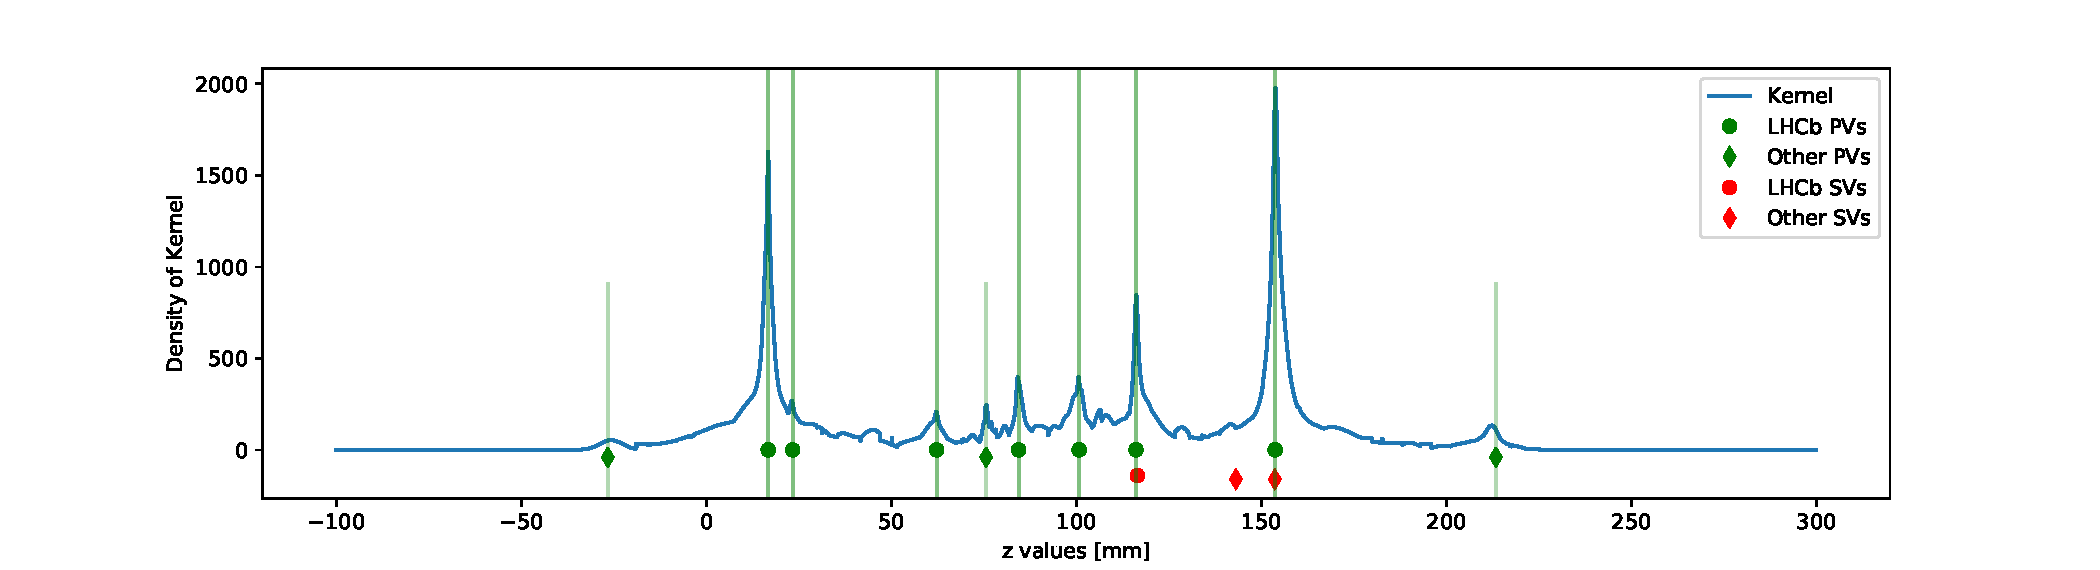
\includegraphics[width=\textwidth, trim=50 30 50 30]{images/kernel_and_pvs.pdf}
\end{center}
\begin{columns}[b]
    \column{.55\textwidth}

    \textcolor{lhcbRed}{Note: All events from toy detector simulation}

    \begin{block}{Human learning}
    \begin{itemize}
        \item Peaks generally correspond to PVs and SVs
    \end{itemize}
    \end{block}

    \column{.45\textwidth}
    \begin{block}{Challenges}
    \begin{itemize}
        \item Vertex may be offset from peak
        \item Vertices interact
    \end{itemize}
    \end{block}
\end{columns}
\end{frame}


\subsection{Target distribution}
\begin{frame}{Target distribution}
\vspace{-.8cm}
\begin{columns}[c]
    \column{.68\textwidth}
    \begin{block}{Build target distribution}
      \begin{itemize}
          \item True PV position as the mean of Gaussian
          \item $\sigma$ (standard deviation) is $\unit[100]{\mu m}$ (simplification)
          \item Fill bins with integrated PDF within $\pm 3$ bins ($\pm \unit[300]{\mu m}$ )
      \end{itemize}
    \end{block}
    \column{.33\textwidth}
      \begin{center}
    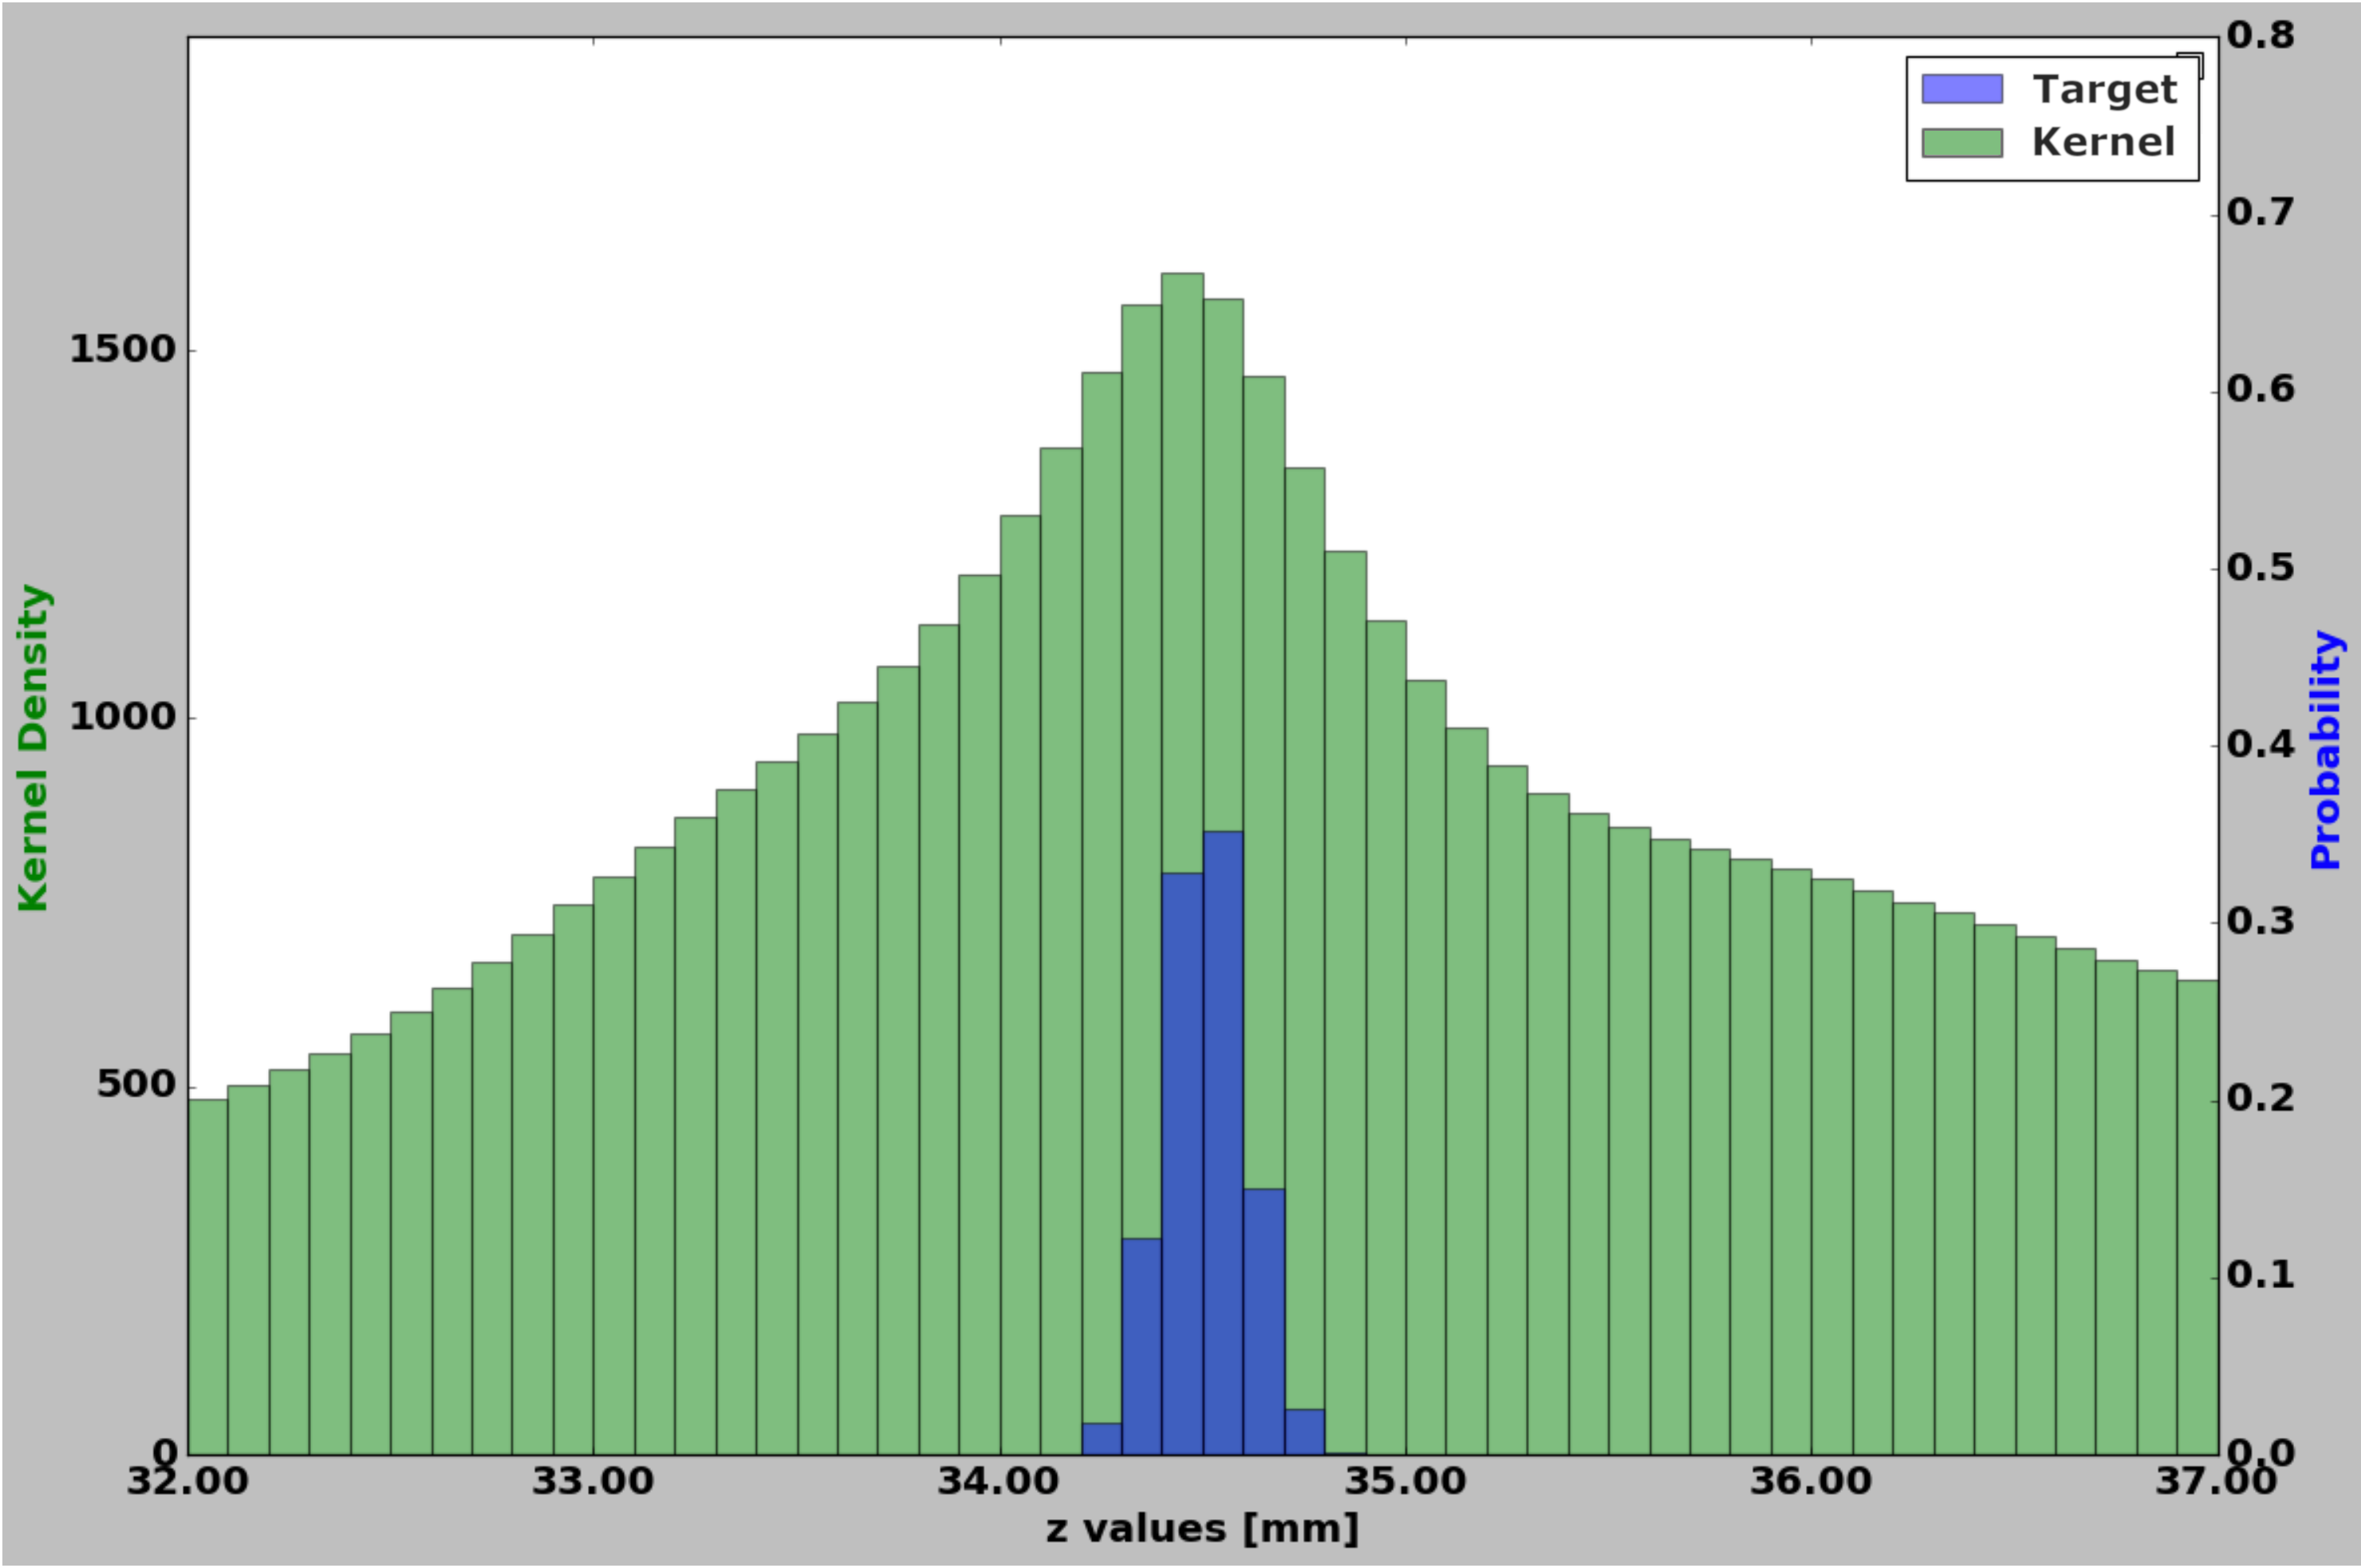
\includegraphics[height=3.3cm, trim=18 0 18 0]{images/T_1_25.png}
  \end{center}
  \end{columns}
  \vspace{-.5cm}
  \begin{columns}
      \column{.33\textwidth}
      \begin{center}
        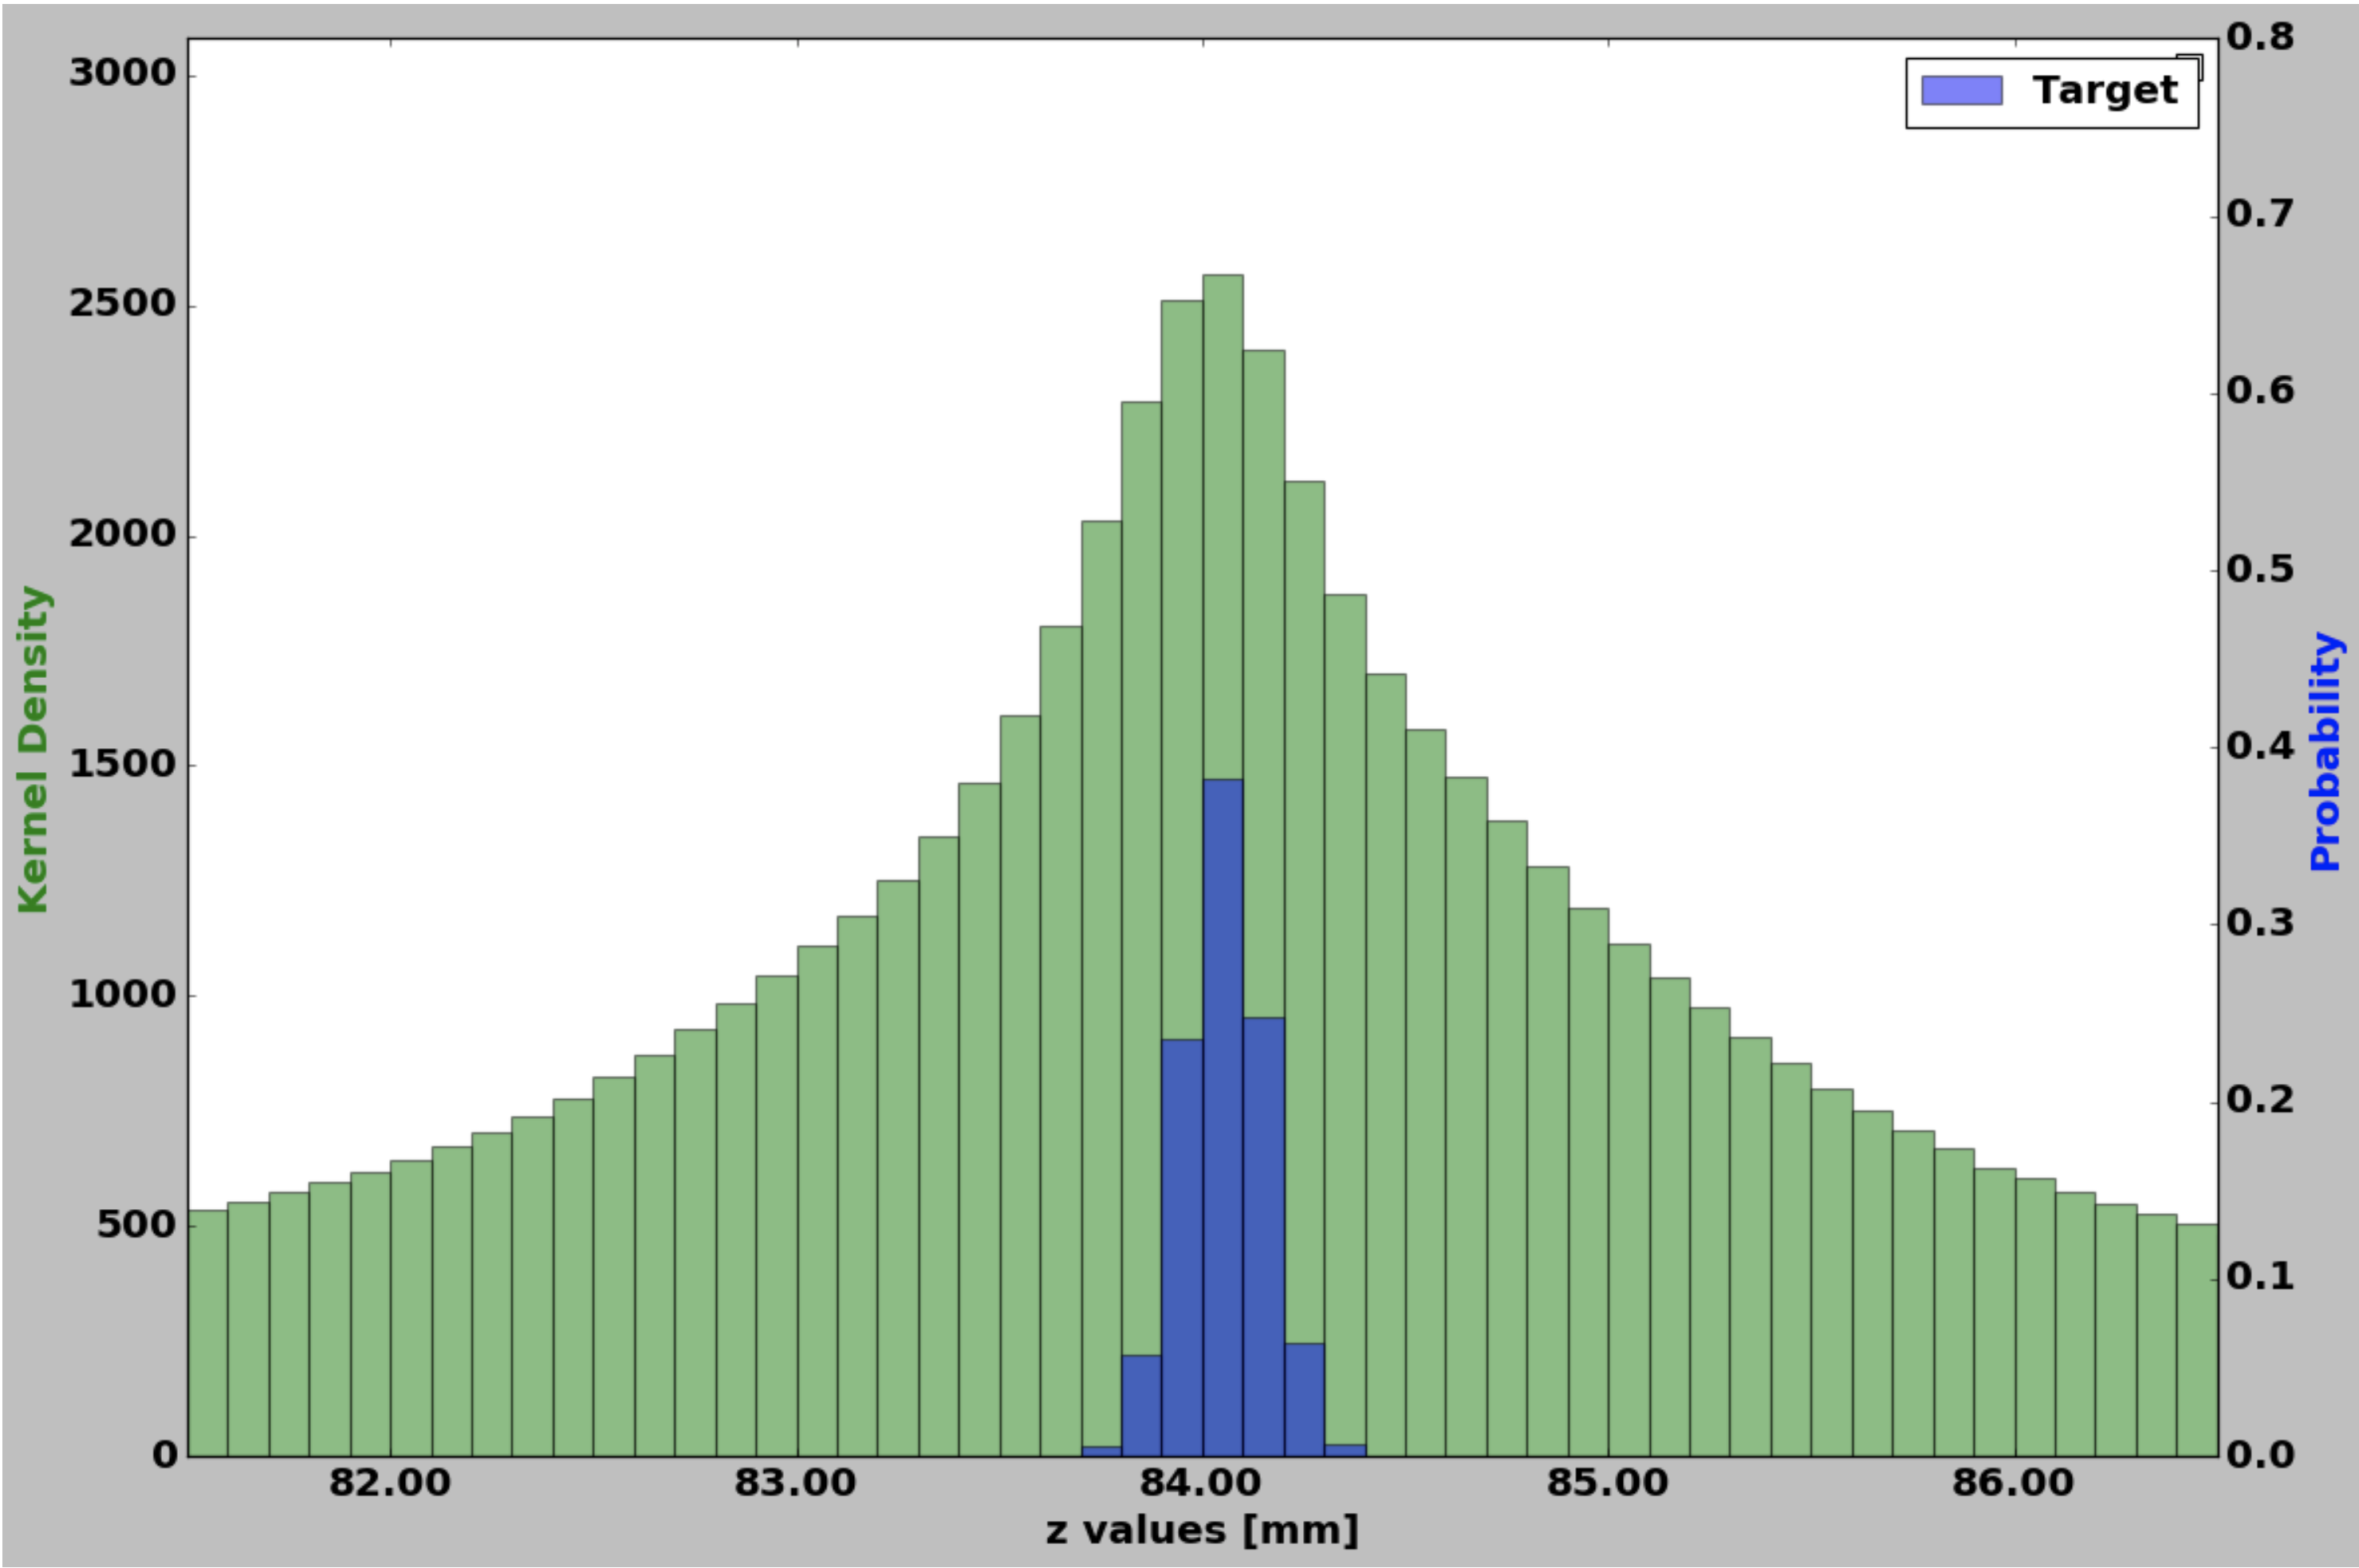
\includegraphics[height=3.3cm,trim=18 0 18 0]{images/T_2_25.png}
      \end{center}
      \column{.33\textwidth}
      \begin{center}
        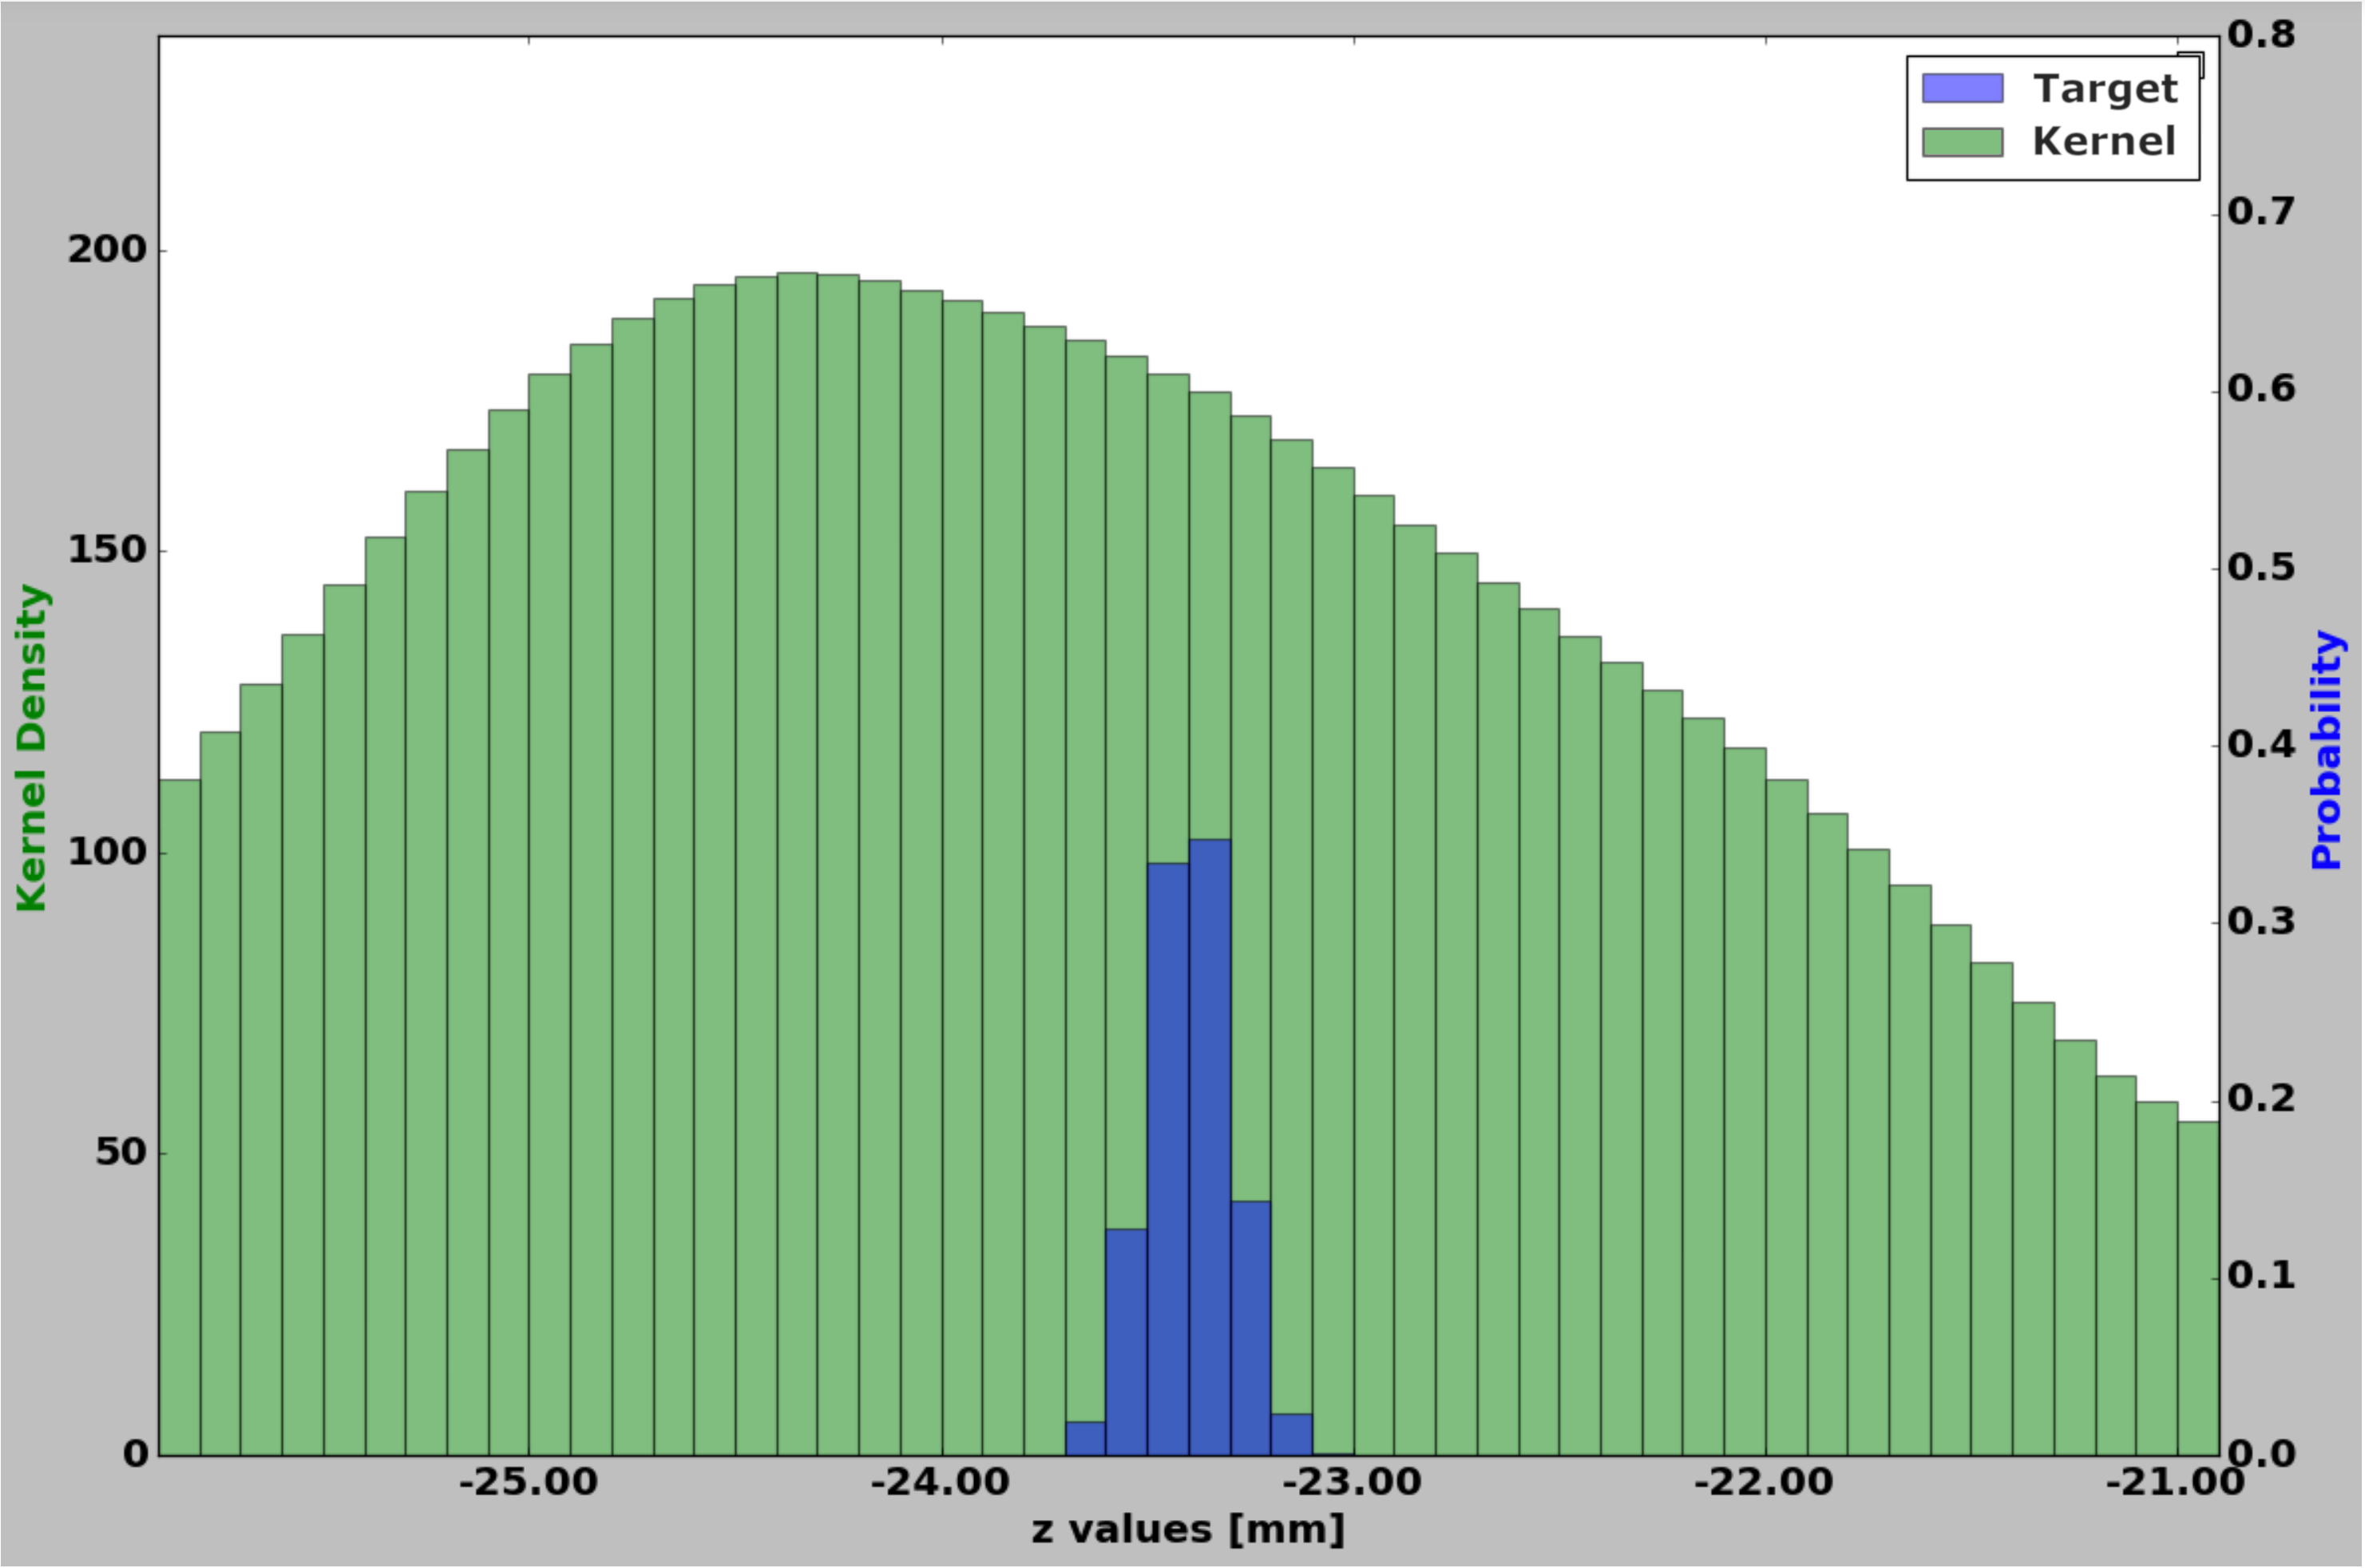
\includegraphics[height=3.3cm,trim=18 0 18 0]{images/T_3_25.png}
      \end{center}
      \column{.33\textwidth}
      \begin{center}
        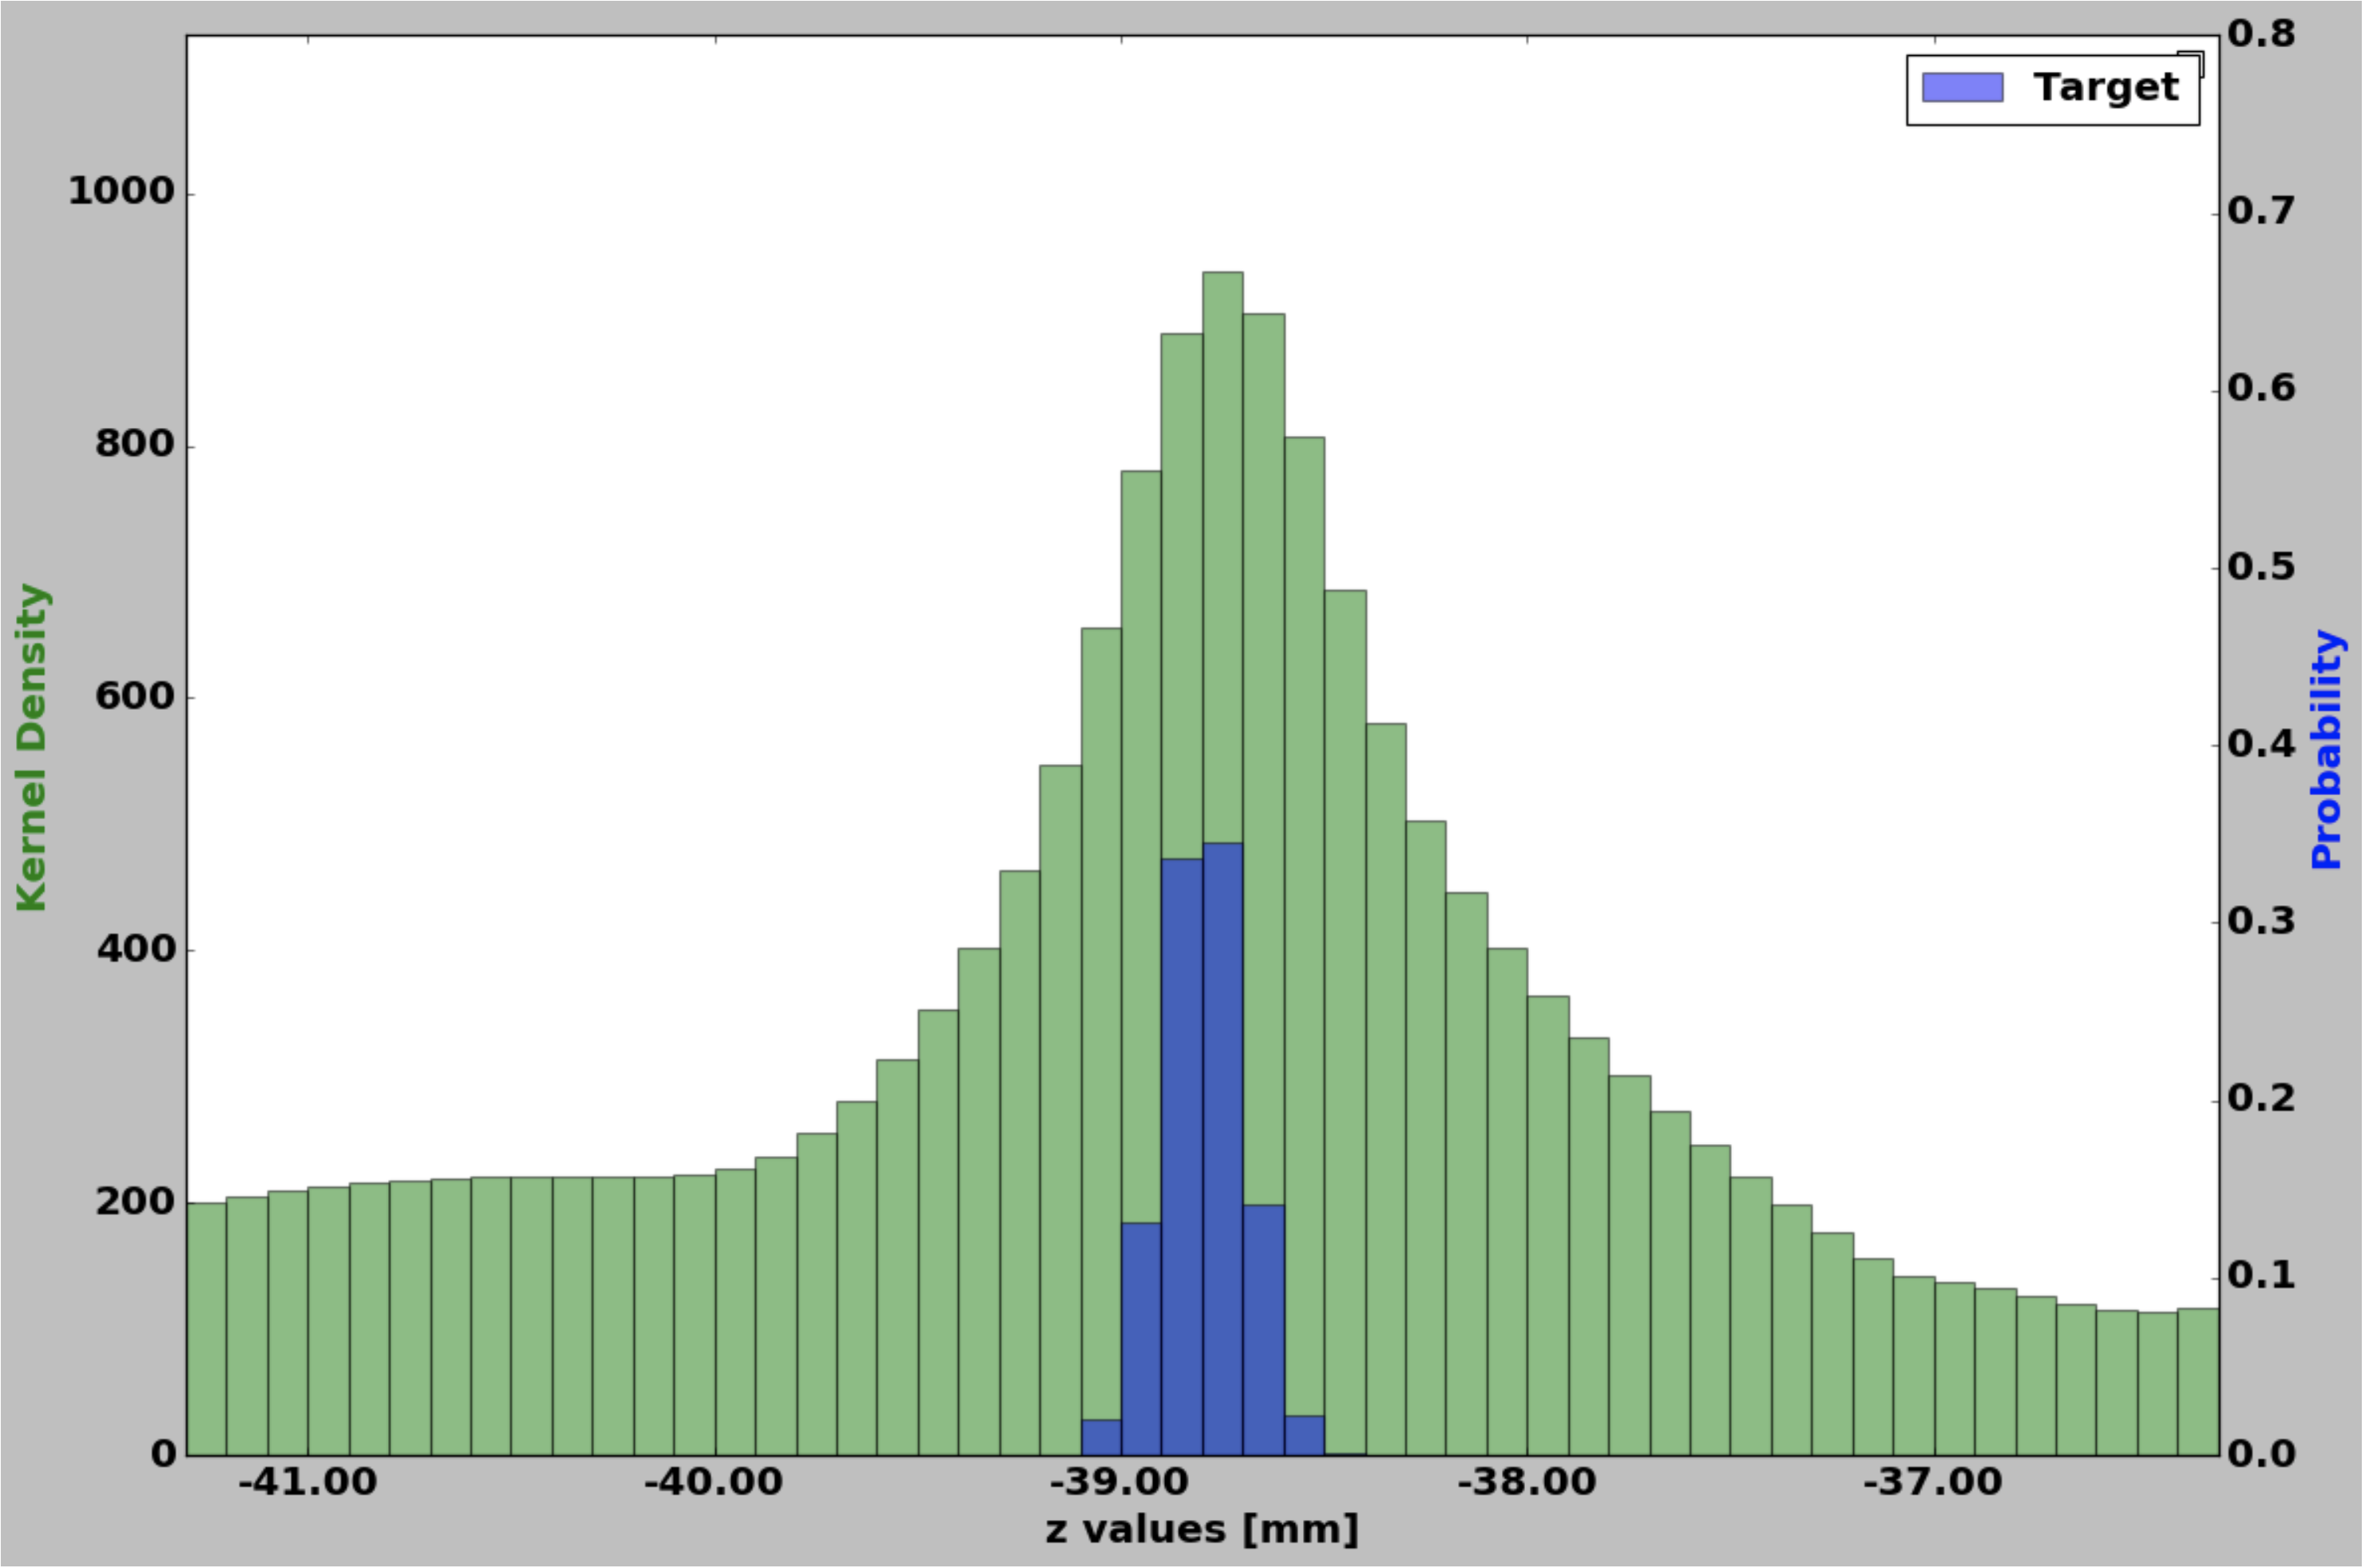
\includegraphics[height=3.3cm,trim=18 0 18 0]{images/T_4_25.png}
      \end{center}
  \end{columns}

% Note: Adding better legend would be nice.

\end{frame}


\subsection{Neural network architecture}
\begin{frame}{Neural network architecture with three convolutional layers}
    %
    % KERNEL_SIZE =   [25, 15, 15, 5, 91]
    % CHANNELS_SIZE = [25, 25, 25, 1, 1]
    % DEFAULTS = {'dropout_1':0.05, 'dropout_2':0.05, 'dropout_3':0.05, 'dropout_4':0.05}
    % FINAL_ACTIVATION = nn.Softplus
    % FC = False
    %

\newcounter{layer}
\setcounter{layer}{0}
\def\wid{3.7}

\begin{center}
\begin{tikzpicture}[
    scale=.77,
    every node/.style={scale=.77}]

% Layer 1
\begin{scope}[xshift=\thelayer*\wid cm]
\node at (0,0) {Inputs};
\foreach \i [count=\xi] in {1,2,3,$\cdots$,25,26,$\cdots$,3998,3999,4000} {
    \node at(0, -\xi/2) [draw, minimum width = 1cm, minimum height = .5cm] {\i};
}

\draw [decorate,decoration={brace,amplitude=10pt}] (.5,-.25) -- (.5,-2.75);
\draw [-latex] (.6, -2.75) -- (.6, -3.2);
\draw [-latex] (.9, -1.5) -- (\wid - 1, -1.5);
\begin{scope}[xshift=.5cm, yshift=-3.5cm]
\node at (0, 0) [right] {Convolution};
\node at (0,  -.6) [right] {Width:};
\node at (.5, -1) [right] {25};
\node at (0, -1.4) [right] {Channels:};
\node at (.5, -1.8) [right] {$1\rightarrow25$};
\end{scope}
\end{scope}
\stepcounter{layer}

% Layer 2
\begin{scope}[xshift=\thelayer*\wid cm]
\node at (0,0) {25 Channels};
% Backing
\foreach \i in {.5,.45,.4,.35,.3,.25,.2,.15,.1,.05} {
\begin{scope}[xshift=-.5cm-\i cm, yshift=-.25cm -\i cm]
\path[fill=white] (0,0) rectangle (1,-5);
\draw [opacity=1-\i*2 + .05, ystep=.5] (0,0) grid (1,-5);
\end{scope}
}
\foreach \i [count=\xi] in {1,2,3,$\cdots$,15,16,$\cdots$,3998,3999,4000} {
    \node at(0, -\xi/2) [draw, fill=white, minimum width = 1cm, minimum height = .5cm] {\i};
}

\draw [decorate,decoration={brace,amplitude=10pt}] (.5,-.25) -- (.5,-2.75);
\draw [-latex] (.6, -2.75) -- (.6, -3.2);
\draw [-latex] (.9, -1.5) -- (\wid - 1, -1.5);
\begin{scope}[xshift=.5cm, yshift=-3.5cm]
\node at (0, 0) [right] {Convolution};
\node at (0,  -.6) [right] {Width:};
\node at (.5, -1) [right] {15};
\node at (0, -1.4) [right] {Channels:};
\node at (.5, -1.8) [right] {$25\rightarrow25$};
\end{scope}
\end{scope}
\stepcounter{layer}

% Layer 3
\begin{scope}[xshift=\thelayer*\wid cm]
\node at (0,0) {25 Channels};
% Backing
\foreach \i in {.5,.45,.4,.35,.3,.25,.2,.15,.1,.05} {
\begin{scope}[xshift=-.5cm-\i cm, yshift=-.25cm -\i cm]
\path[fill=white] (0,0) rectangle (1,-5);
\draw [opacity=1-\i*2 + .05, ystep=.5] (0,0) grid (1,-5);
\end{scope}
}
\foreach \i [count=\xi] in {1,2,3,$\cdots$,15,16,$\cdots$,3998,3999,4000} {
    \node at(0, -\xi/2) [draw, fill=white, minimum width = 1cm, minimum height = .5cm] {\i};
}

\draw [decorate,decoration={brace,amplitude=10pt}] (.5,-.25) -- (.5,-2.75);
\draw [-latex] (.6, -2.75) -- (.6, -3.2);
\draw [-latex] (.9, -1.5) -- (\wid - 1, -1.5);
\begin{scope}[xshift=.5cm, yshift=-3.5cm]
\node at (0, 0) [right] {Convolution};
\node at (0,  -.6) [right] {Width:};
\node at (.5, -1) [right] {15};
\node at (0, -1.4) [right] {Channels:};
\node at (.5, -1.8) [right] {$25\rightarrow25$};
\end{scope}
\end{scope}
\stepcounter{layer}

% Layer 4
\begin{scope}[xshift=\thelayer*\wid cm]
\node at (0,0) {15 Channels};
% Backing
\foreach \i in {.5,.45,.4,.35,.3,.25,.2,.15,.1,.05} {
\begin{scope}[xshift=-.5cm-\i cm, yshift=-.25cm -\i cm]
\path[fill=white] (0,0) rectangle (1,-5);
\draw [opacity=1-\i*2 + .05, ystep=.5] (0,0) grid (1,-5);
\end{scope}
}
\foreach \i [count=\xi] in {1,2,3,$\cdots$,5,6,$\cdots$,3998,3999,4000} {
    \node at(0, -\xi/2) [draw, fill=white, minimum width = 1cm, minimum height = .5cm] {\i};
}

\draw [decorate,decoration={brace,amplitude=10pt}] (.5,-.25) -- (.5,-2.75);
\draw [-latex] (.6, -2.75) -- (.6, -3.2);
\draw [-latex] (.9, -1.5) -- (\wid - 1, -1.5);
\begin{scope}[xshift=.5cm, yshift=-3.5cm]
\node at (0, 0) [right] {Convolution};
\node at (0,  -.6) [right] {Width:};
\node at (.5, -1) [right] {5};
\node at (0, -1.4) [right] {Channels:};
\node at (.5, -1.8) [right] {$25\rightarrow1$};
\end{scope}
\end{scope}
\stepcounter{layer}

% Layer 5
\begin{scope}[xshift=\thelayer*\wid cm - .5 cm]
\node at (0,0) {1 Channel};
% Backing
%\foreach \i in {.4,.3,.2,.1} {
%\begin{scope}[xshift=-.5cm-\i cm, yshift=-.25cm -\i cm]
%\path[fill=white] (0,0) rectangle (1,-5);
%\draw [opacity=1-\i*2, ystep=.5] (0,0) grid (1,-5);
%\end{scope}
%}
\foreach \i [count=\xi] in {1,2,3,$\cdots$,91,92,$\cdots$,3998,3999,4000} {
    \node at(0, -\xi/2) [draw, fill=white, minimum width = 1cm, minimum height = .5cm] {\i};
}

\draw [decorate,decoration={brace,amplitude=10pt}] (.5,-.25) -- (.5,-2.75);
\draw [-latex] (.6, -2.75) -- (.6, -3.2);
\draw [-latex] (.9, -1.5) -- (\wid - 1, -1.5);
\begin{scope}[xshift=.5cm, yshift=-3.5cm]
\node at (0, 0) [right] {Convolution};
\node at (0,  -.6) [right] {Width:};
\node at (.5, -1) [right] {91};
\node at (0, -1.4) [right] {Channels:};
\node at (.5, -1.8) [right] {$1\rightarrow1$};
\end{scope}
\end{scope}
\stepcounter{layer}

% Layer Output
\begin{scope}[xshift=\thelayer*\wid cm - 1 cm]
\node at (0,0) {Output};
\foreach \i [count=\xi] in {1,2,3,4,5,$\cdots$,3997,3998,3999,4000} {
    \node at(0, -\xi/2) [draw, fill=white, minimum width = 1cm, minimum height = .5cm] {\i};
}
\end{scope}
\stepcounter{layer}

\begin{scope}[xshift=-.5cm, yshift=-7.5cm]

% Loop as needed
\foreach \i in {\wid * 0.5,\wid * 1.5, \wid * 2.5, \wid * 3.5} {
\begin{scope}[xshift=\i cm]
\draw [step=.25] (-1.2, .05) grid (1.2, -.05);
\draw [step=.25] (-.05, -.2) grid (.05, 1.4);
\draw [black, latex-latex] (-1.3, 0) node[above] {-x} -- (1.3, 0) node[above] {x};
\draw [black, latex-latex] (0, -.3)  -- (0, 1.3) node[left] {y};
\draw [thick, blue](-1.3, -.1) -- (0, 0) -- (1.3,1.3);
\node at (0, -.6) {Leaky relu};
\end{scope}
}

\begin{scope}[xshift=\wid * 4.5 cm - .25 cm]
\draw [step=.25] (-1.2, .05) grid (1.2, -.05);
\draw [step=.25] (-.05, -.2) grid (.05, 1.4);
\draw [black, latex-latex] (-1.3, 0) node[above] {-x} -- (1.3, 0) node[above] {x};
\draw [black, latex-latex] (0, -.3)  -- (0, 1.3) node[left] {y};
\draw [thick, blue, smooth]  plot coordinates {
    (-1.5, 0)
	(0, .25)
	(1.3, 1.3)};
\node at (0, -.6) {Softplus};
\end{scope}

\end{scope}

\end{tikzpicture}
\end{center}
\end{frame}


\subsection{Cost function}
\begin{frame}{Cost function}
    \begin{block}{Approach}
      \begin{itemize}
         \item
            Should be similar to Cross-Entropy for $ y \to 0 $,
           $ y \to 1 $;
             $ \color{brickred} \textrm{cost} = - \left (y \ln \hat{y} + (1-y) \ln (1 - \hat{y}) \right )  $
         \item
          Should be symmetric with respect to  $ r = ( \hat y/y  )$ \& $ 1/r $
     \end{itemize}
     \vspace{-.3cm}

     \[
     r_i \equiv (\hat{y_i} + \epsilon)/ (y_i + \epsilon)
     \quad
     z_i \equiv \frac{2 \, r_i }{r_i + 1/r_i}
     \]
    \end{block}

  \begin{columns}[c]
    \column{0.33\textwidth}
    \centering
    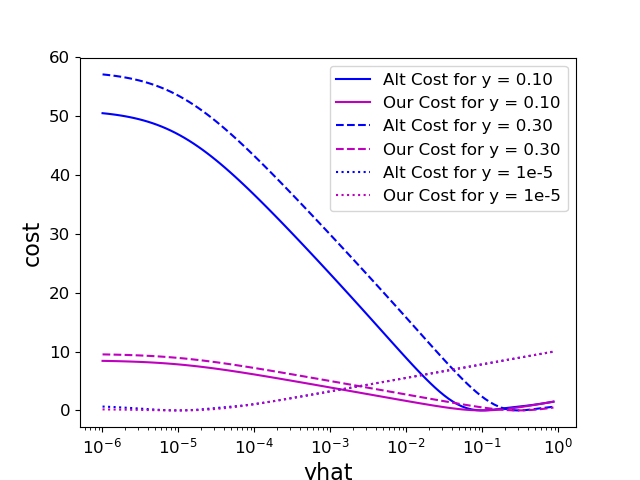
\includegraphics[width=\textwidth]{images/AltCostPlot_181015.png}
    \column{0.33\textwidth}
    \centering
    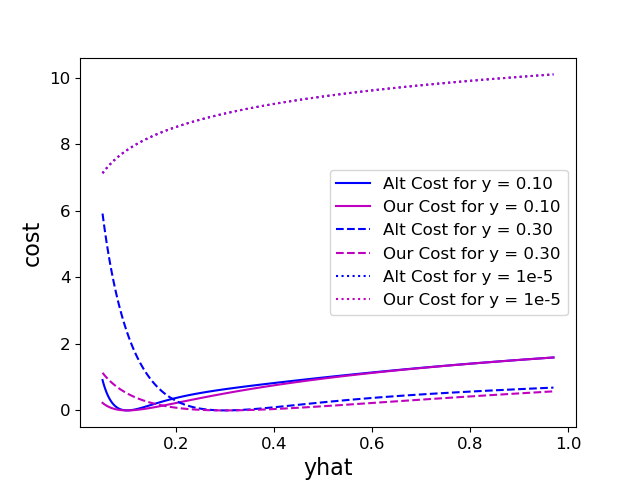
\includegraphics[width=\textwidth]{images/AltCostPlot_181015_linearA.png}
    \column{0.33\textwidth}
    \centering
    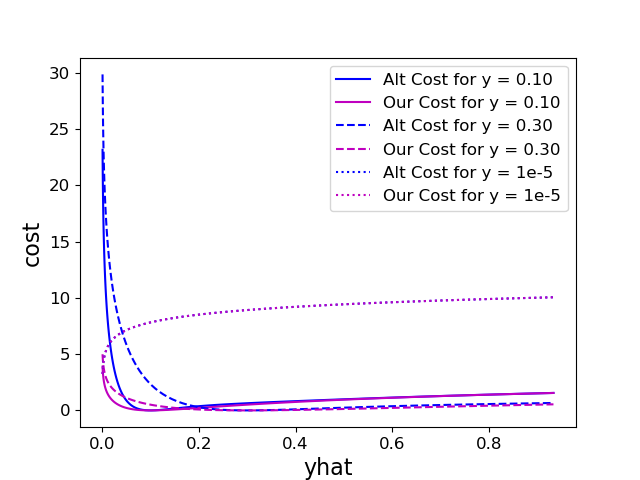
\includegraphics[width=\textwidth]{images/AltCostPlot_181015_linear.png}
    \end{columns}
\end{frame}


%%%%%%%%%%%%%%%%%%%%%%%%%%%%%%%%%%%%%%%%%%%%%%%%%%%%%%%%%%%%%%%%%%%%%%%%%%%%%%%

\section{Results}

\subsection{Prediction plots}
\begin{frame}{Compare predictions with targets: When it works}
  \begin{columns}[c]
    \column{.5\textwidth}
        \begin{center}
           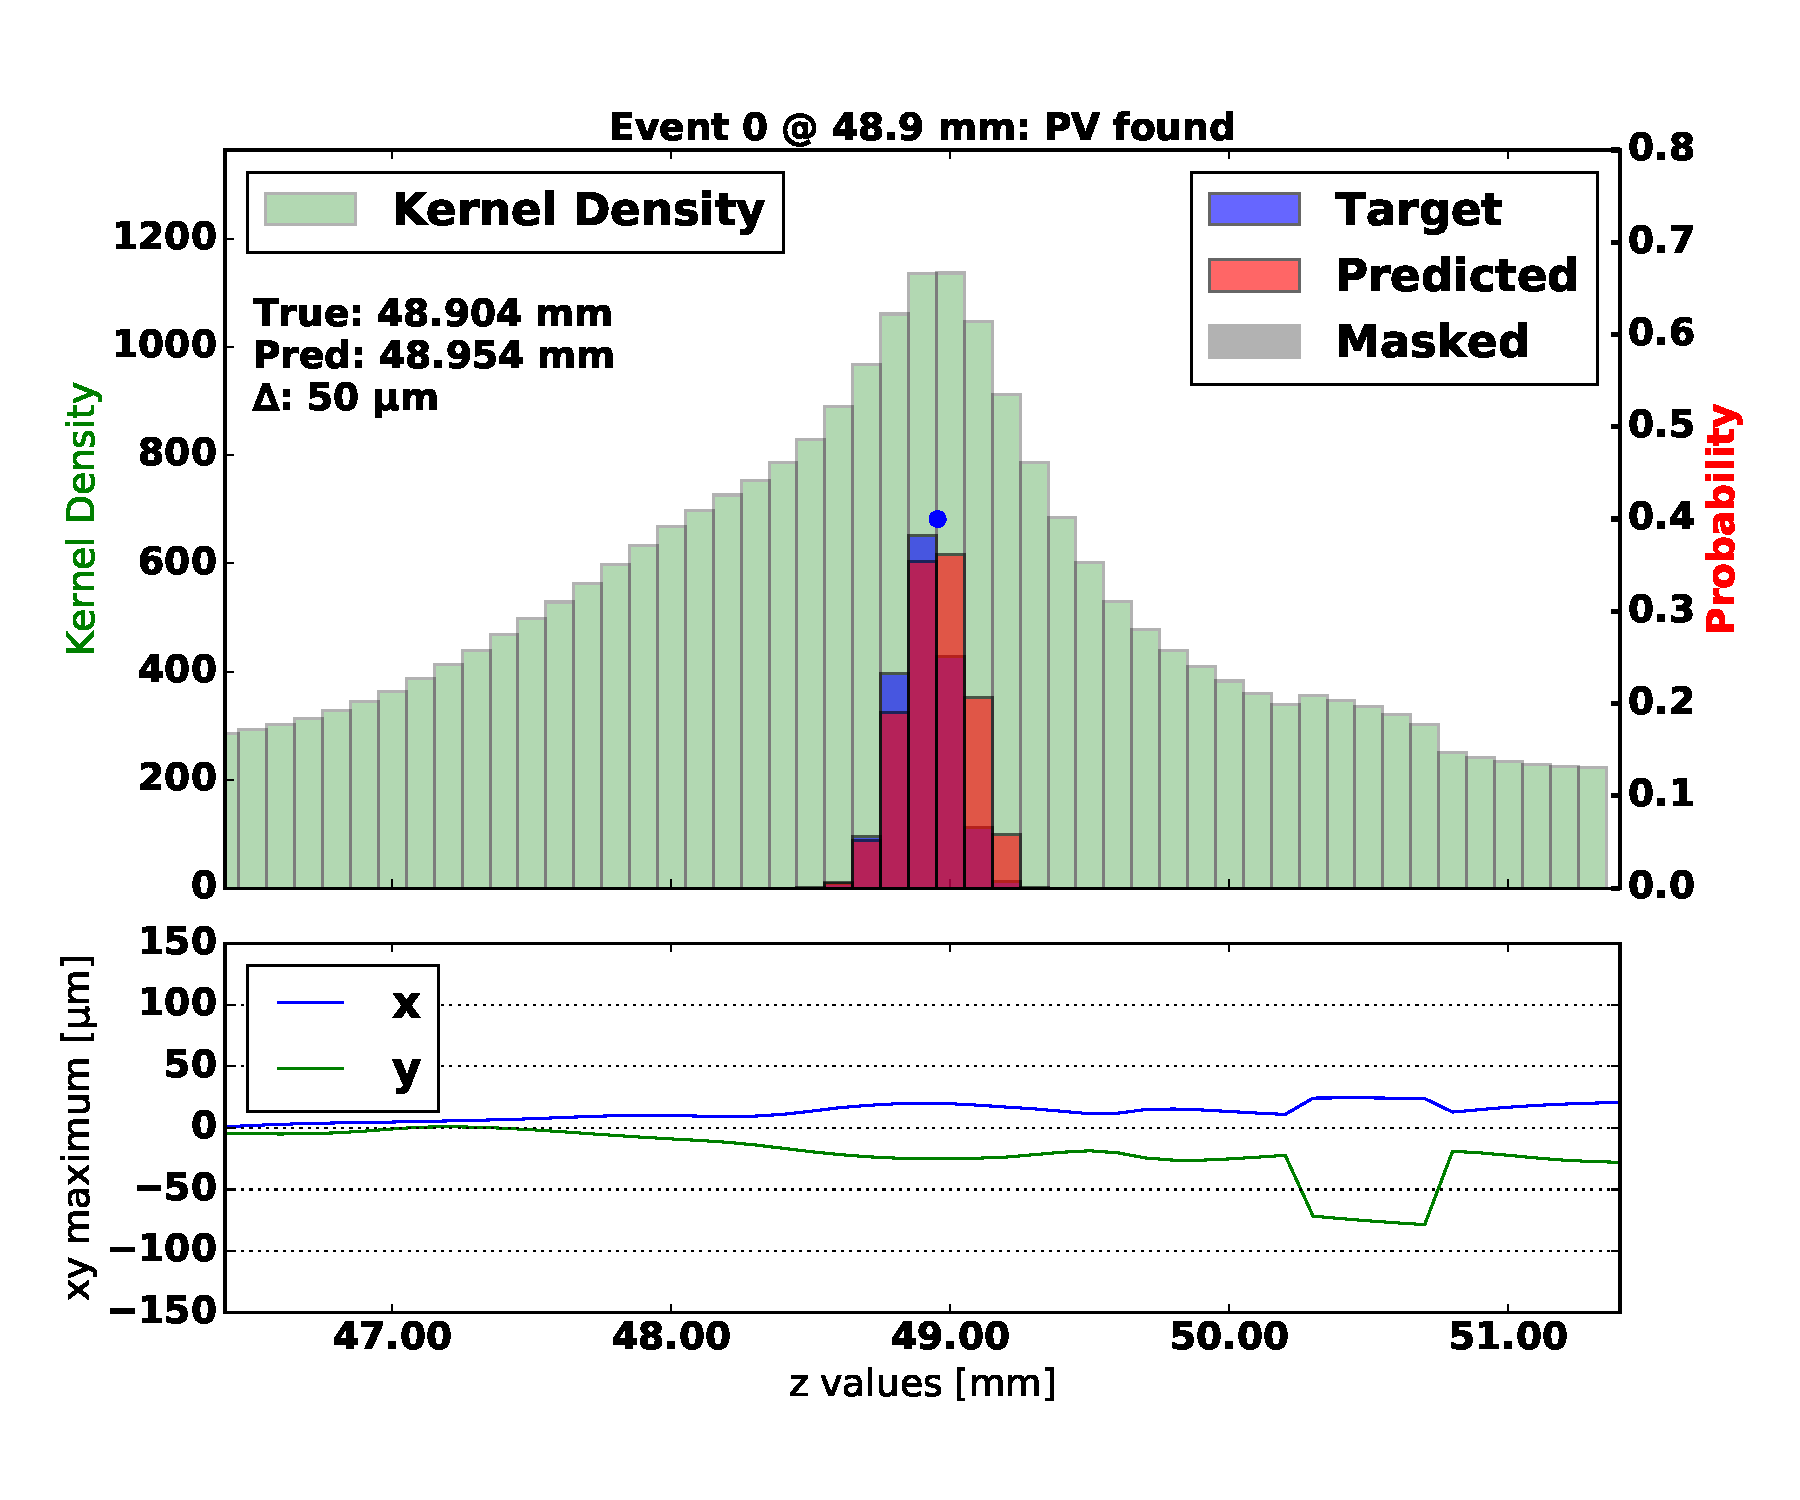
\includegraphics[width=1\textwidth, trim=60 40 60 20]{images/07Jan19_AltCNN4Layer_D35_sp_02.pdf}

           \textbf{\color{lhcbBlue}\large PV found example}
       \end{center}
   \column{.5\textwidth}
       \begin{center}
           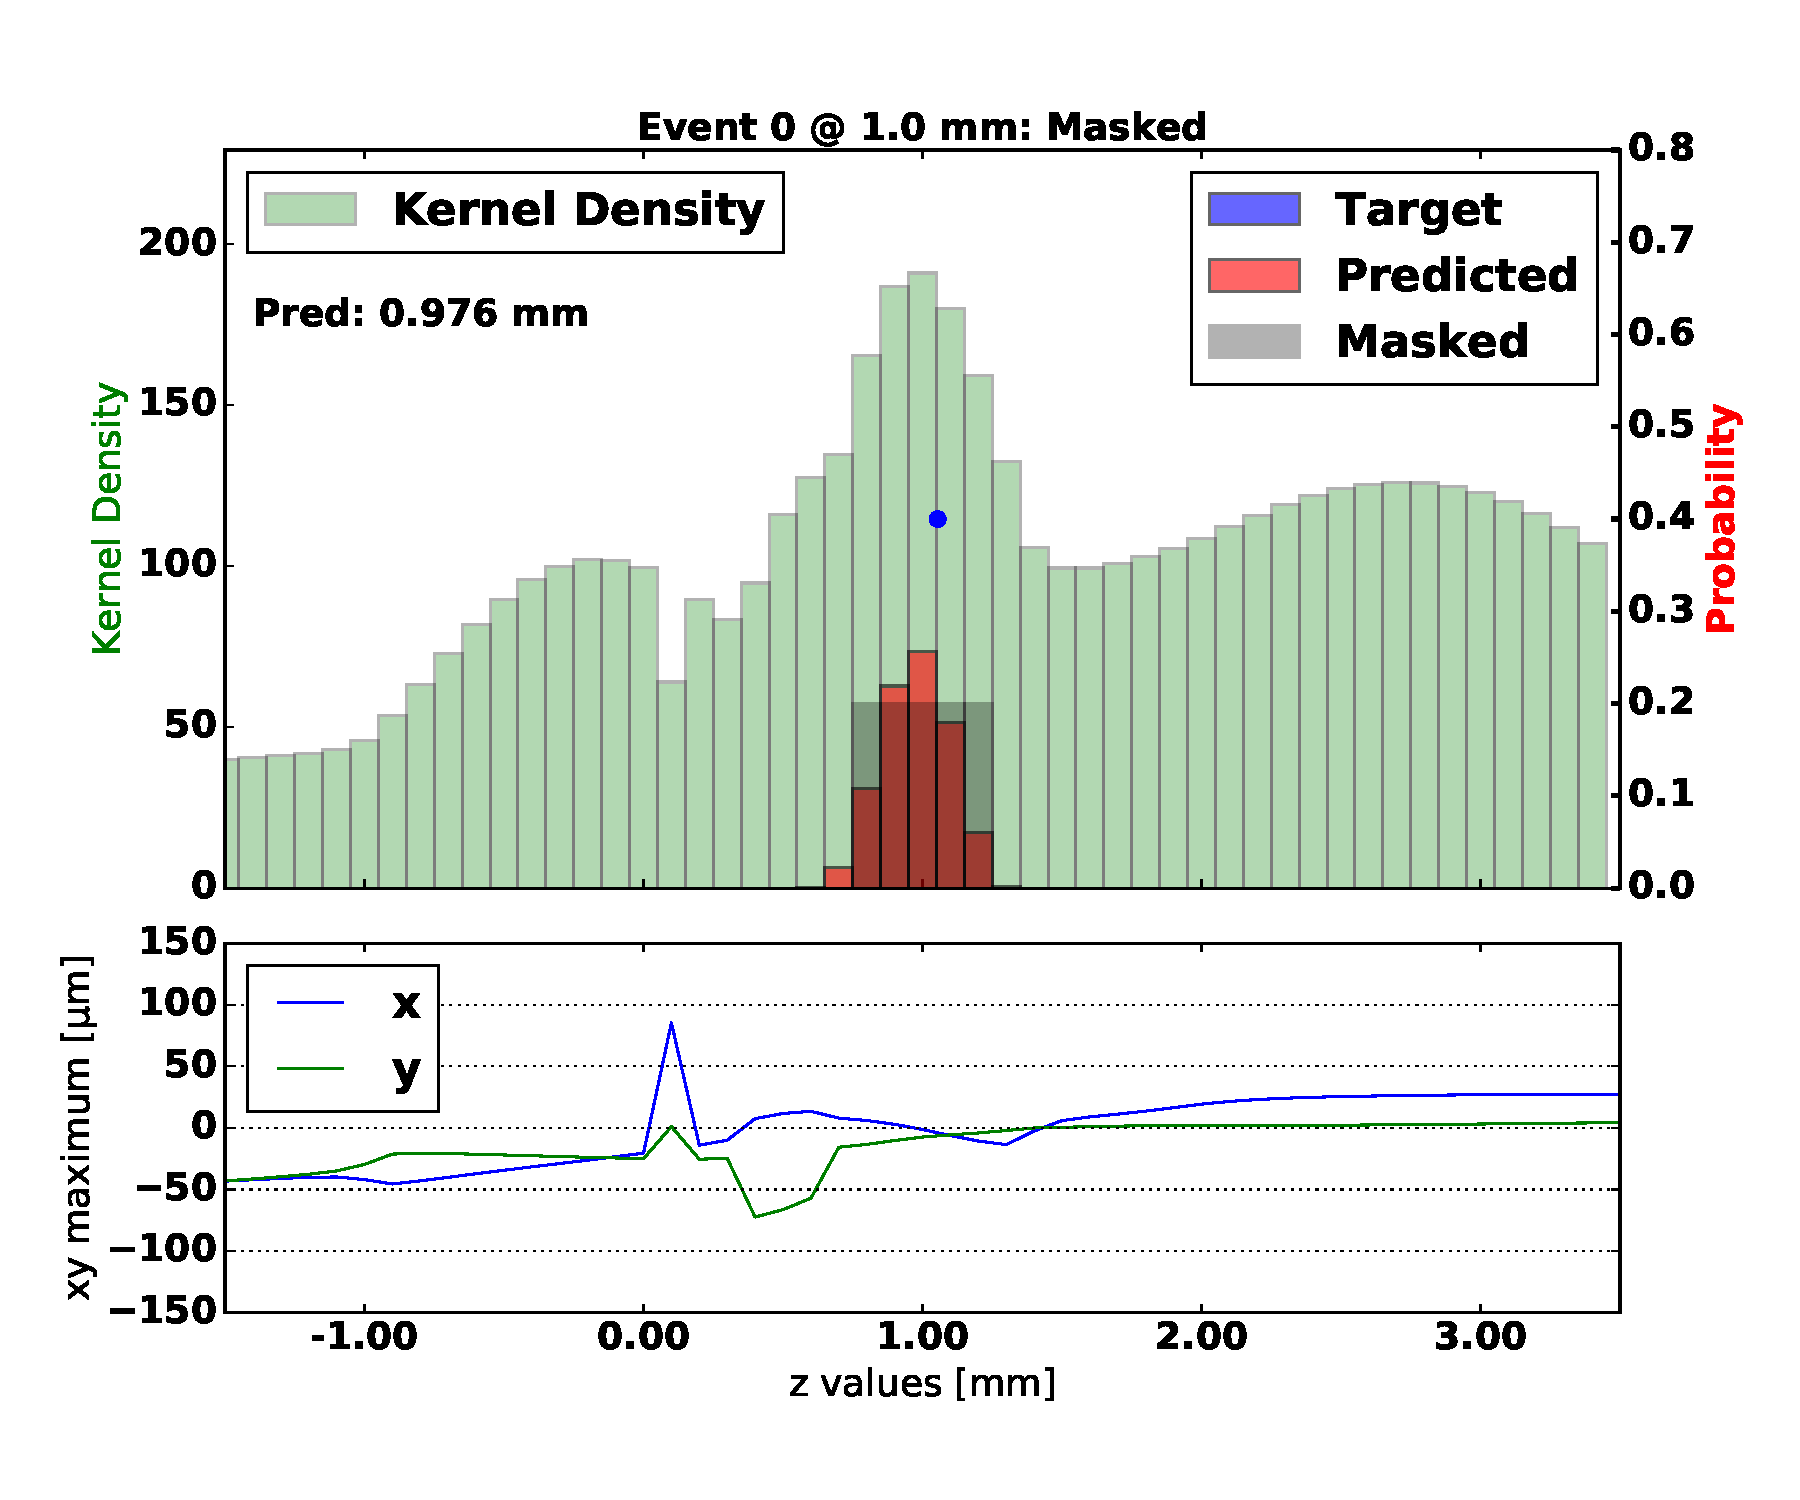
\includegraphics[width=1\textwidth, trim=60 40 60 20]{images/07Jan19_AltCNN4Layer_D35_sp_01.pdf}

           \textbf{\color{lhcbBlue}\large Masked (<5 tracks) example}
       \end{center}
  \end{columns}
\end{frame}


\begin{frame}{Compare predictions with targets: When it fails}
  \begin{columns}[c]
    \column{.5\textwidth}
        \begin{center}
           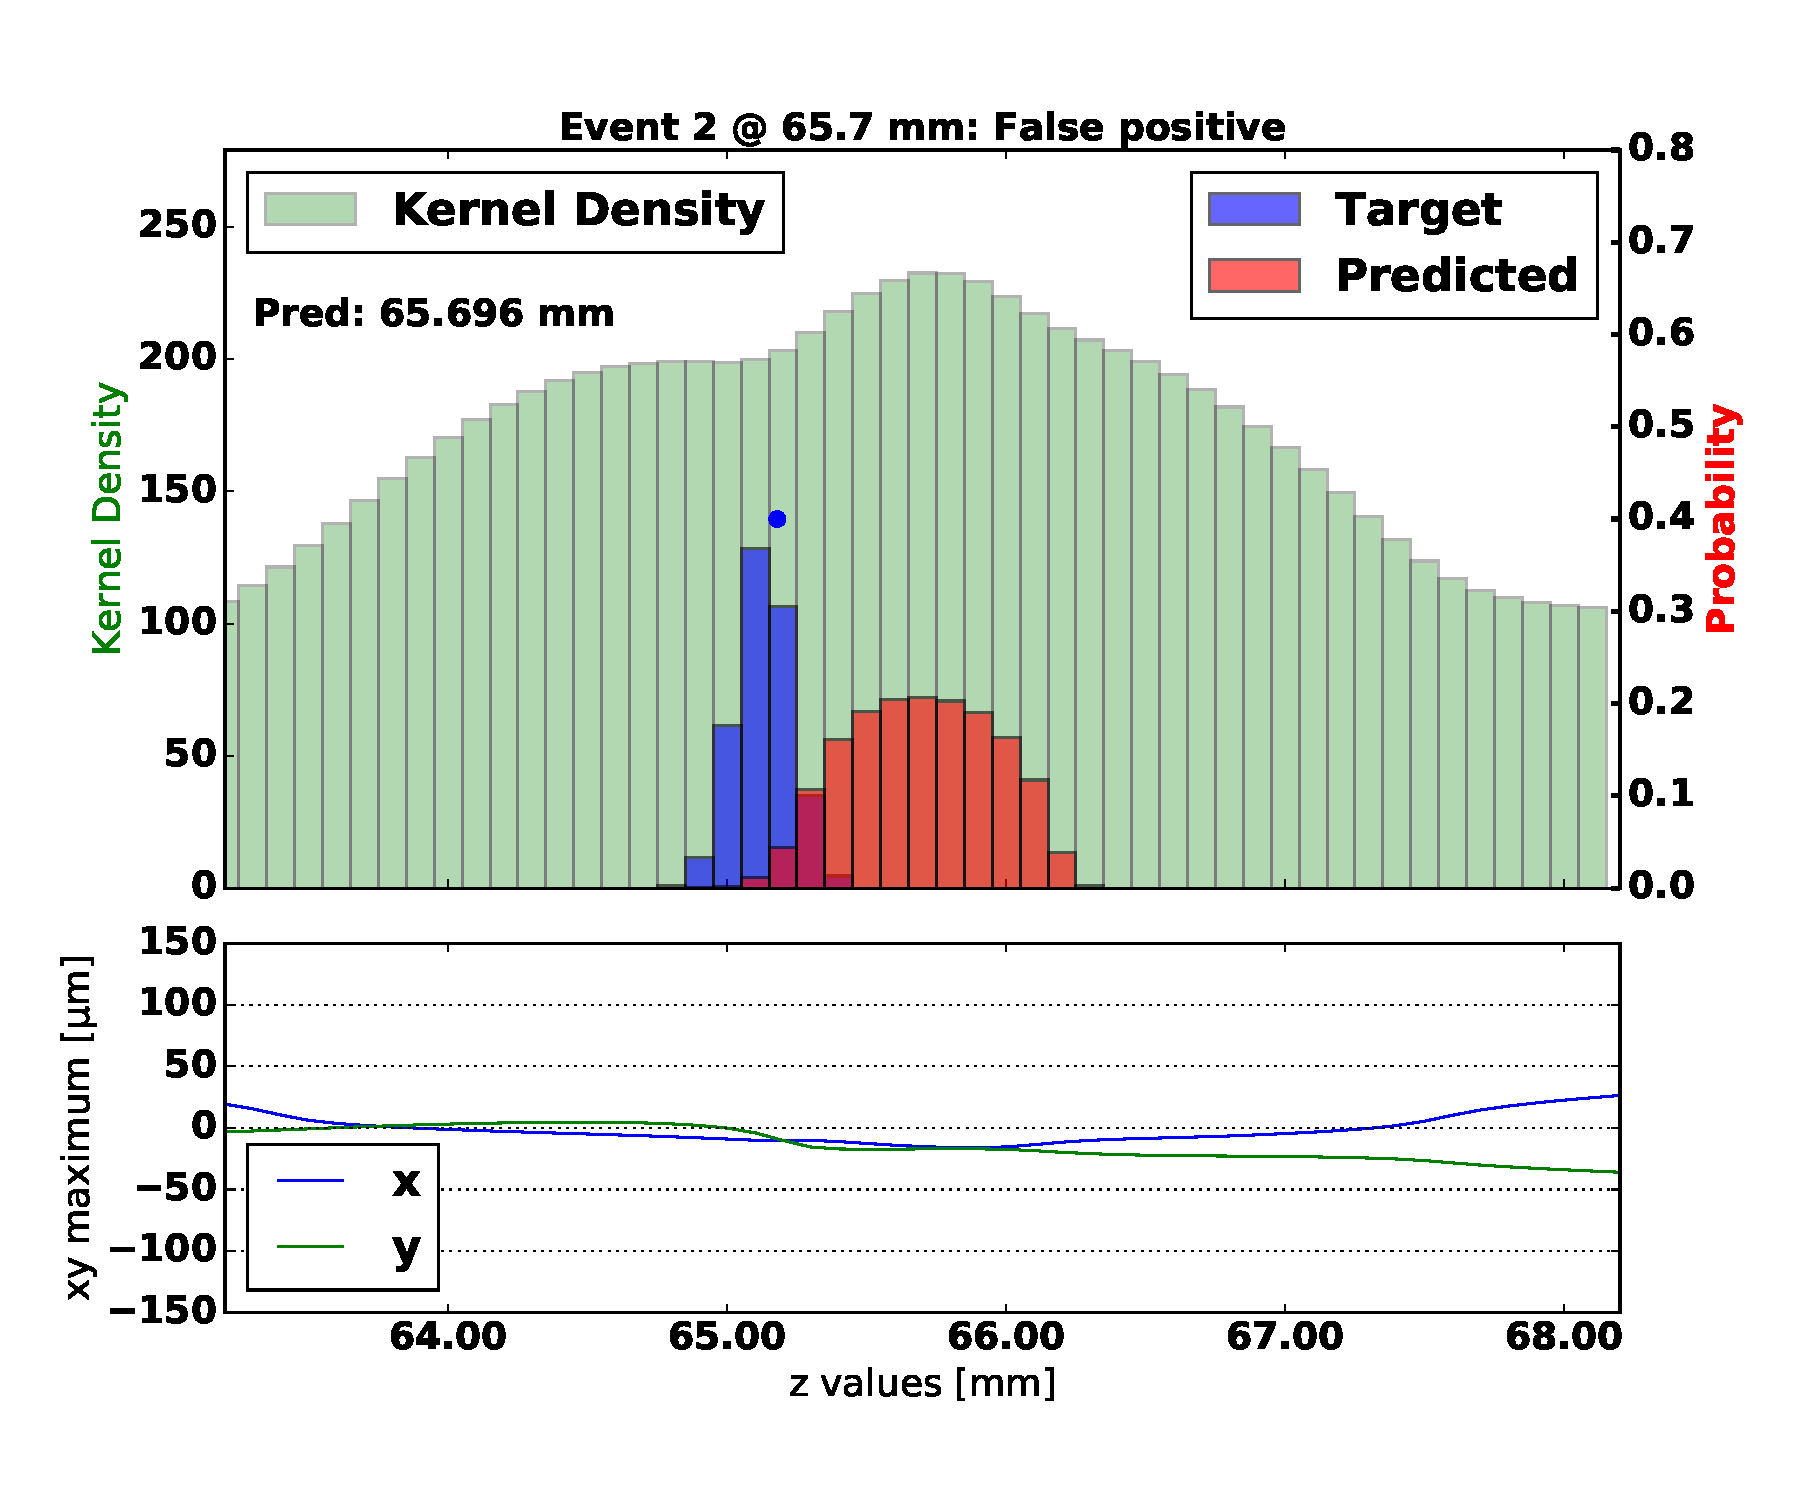
\includegraphics[width=1\textwidth, trim=60 40 60 20]{images/07Jan19_AltCNN4Layer_D35_sp_10.pdf}

           \textbf{\color{lhcbRed}\large False Positive example}
        \end{center}
    \column{.5\textwidth}
        \begin{center}
           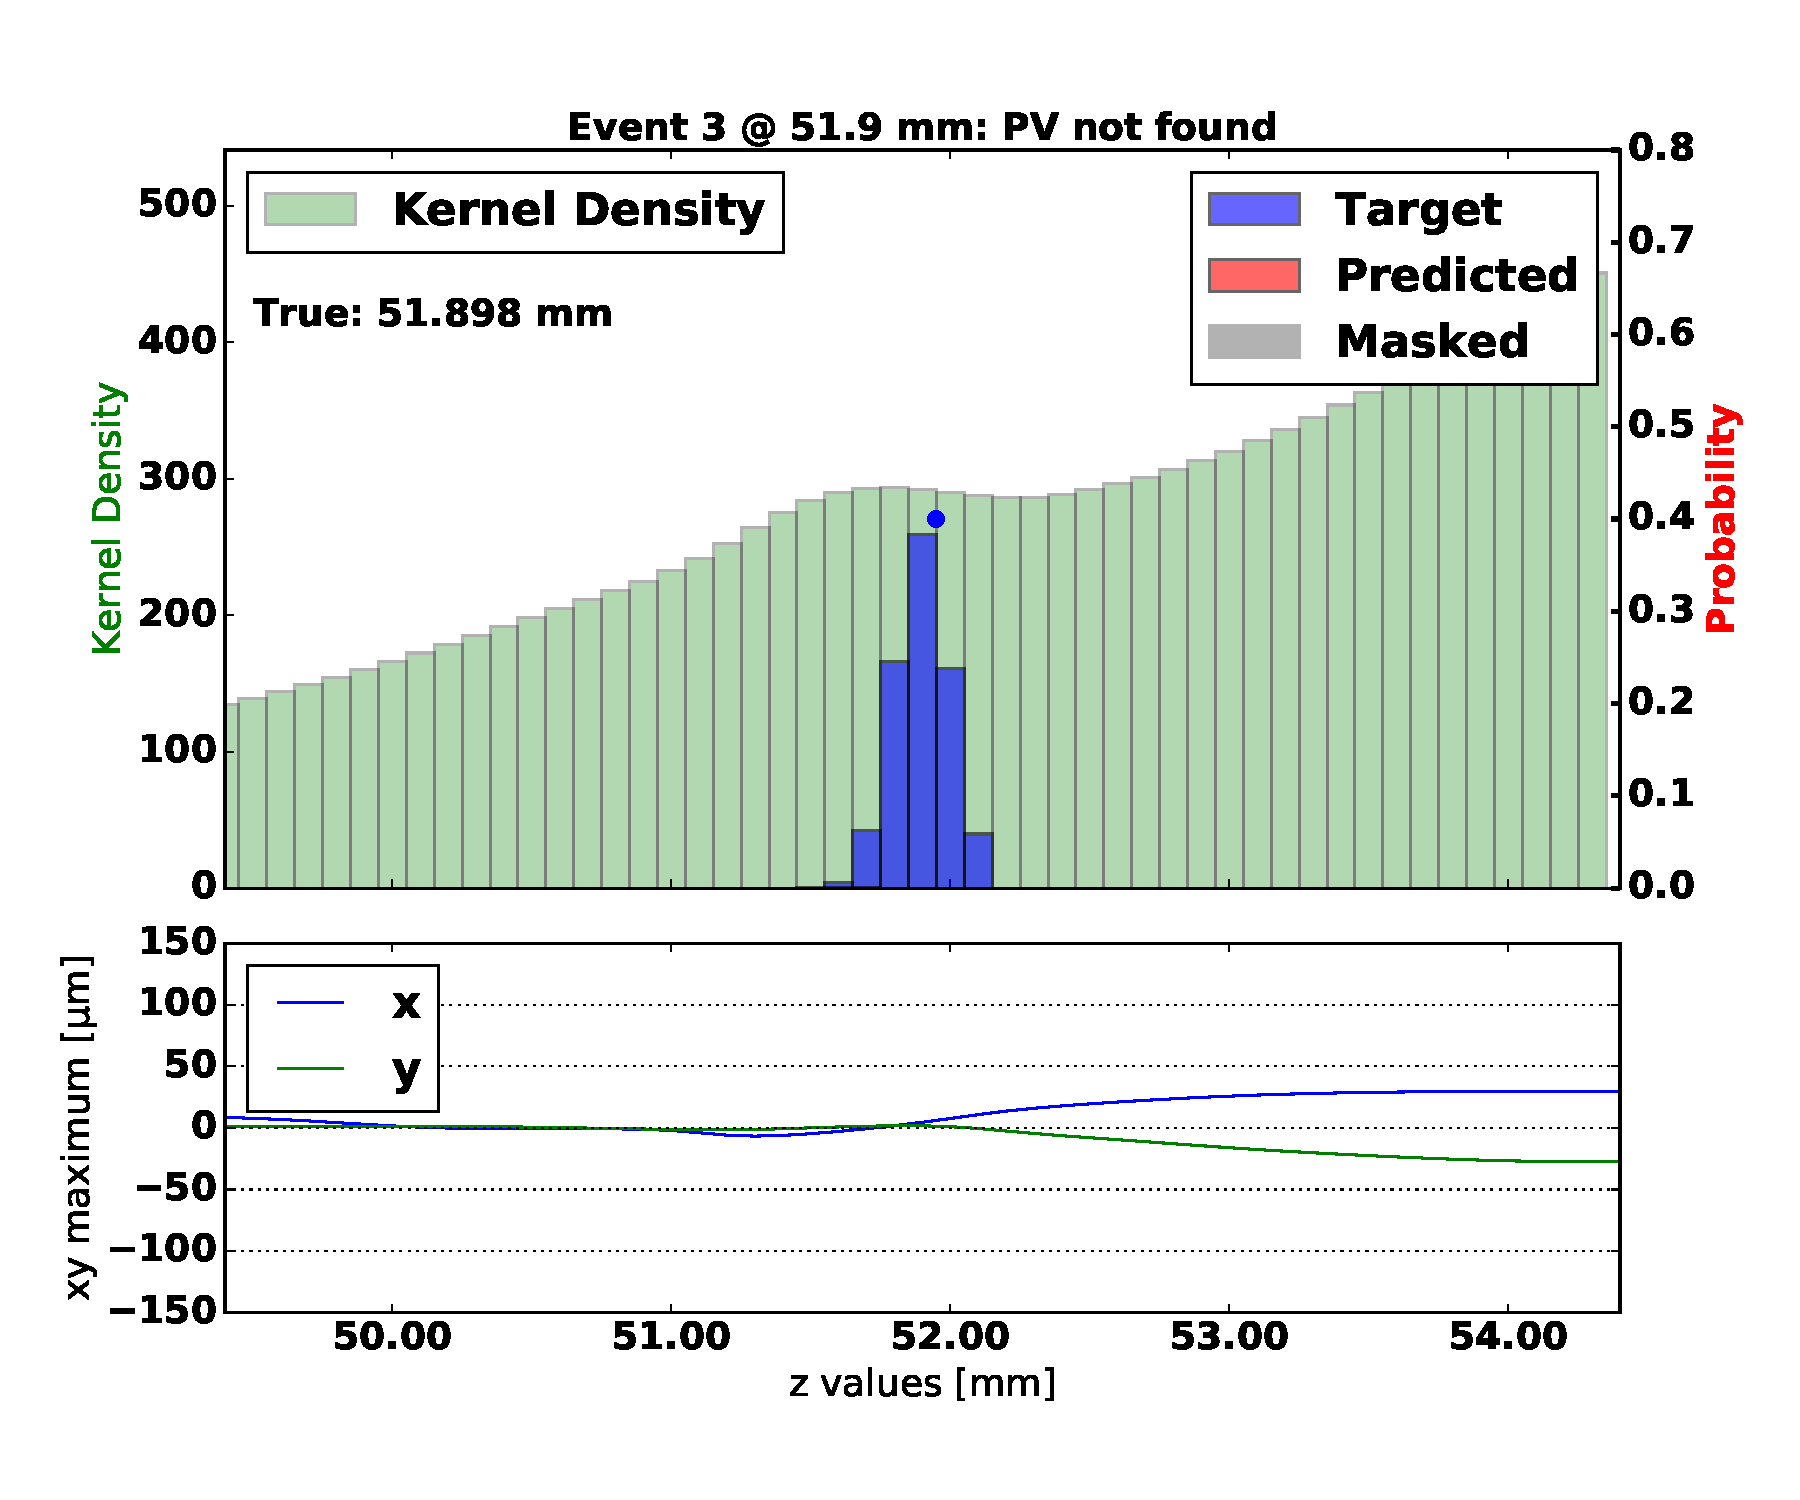
\includegraphics[width=1\textwidth, trim=60 40 60 20]{images/07Jan19_AltCNN4Layer_D35_sp_15.pdf}

           \textbf{\color{lhcbRed}\large PV not found example}
       \end{center}
  \end{columns}
\end{frame}


\subsection{Quantitative results}
\begin{frame}{Efficiencies and false positive rates}
\begin{table}[]
\centering
\begin{tabular}{cccc}
parameter & 2 CVN Layers &
3 CVN Layers & 4 CVN Layers \\ [0.3em]

$\epsilon \textrm{(Efficiency)}
 = \frac{\mbox{TP}}{\mbox{TP} + \mbox{FN}} $
&  $ \approx 58\% $  & $ \approx 70\% $ & $ \approx 75\% $ \\ [0.3em]
$ \textrm{False Positive rate}
 = \frac{\mbox{FP}}{\mbox{number of events}} $
 &  $\approx 0.07 $ & $\approx 0.08 $  & $ \approx 0.13 $ \\
 \end{tabular}
\end{table}
 \vskip -0.05in
  \begin{table}[]
      \centering
      \begin{tabular}{c|cc}
         & Found & Not found \\ \midrule
         Real PV & True positive & False negative\\
         Not a real PV & False positive & True negative
      \end{tabular}
  \end{table}
  \vskip -0.15in
  \begin{block}{True Positive}
    \begin{itemize}
    	\item search $ \pm 5 $ bins ($ \pm 500 \mu $m) around a real PV
    	\item at least 3 (4) bins with predicted probability
    	   $ > 1\% $ and
    	   integrated probability $ > 20\%$.
    \end{itemize}

    \end{block}
    \begin{block}{False Positive}
    \begin{itemize}
        \item
           at least 3 (4) bins with individual probabilities $ > 1\% $ and
          integrated probability $ > 20\%$.
        \item
        no real PV within $ \pm 5 $ bins ($ \pm 500 \mu $m) of that cluster.
    \end{itemize}
  \end{block}
\end{frame}


\subsection{New quantitative results}
\begin{frame}{Performance}
\begin{columns}
\column{.5\textwidth}
<plot of eff vs. nTracks>
\column{.5\textwidth}
<plot of eff vs. FP rate>
\end{columns}
\end{frame}


%%%%%%%%%%%%%%%%%%%%%%%%%%%%%%%%%%%%%%%%%%%%%%%%%%%%%%%%%%%%%%%%%%%%%%%%%%%%%%%

\section{Future plans}

\subsection{Future plans and Conclusions}
\begin{frame}{Conclusions and plans}
    \begin{tikzpicture}[overlay, remember picture]
        \node at (current page.center) {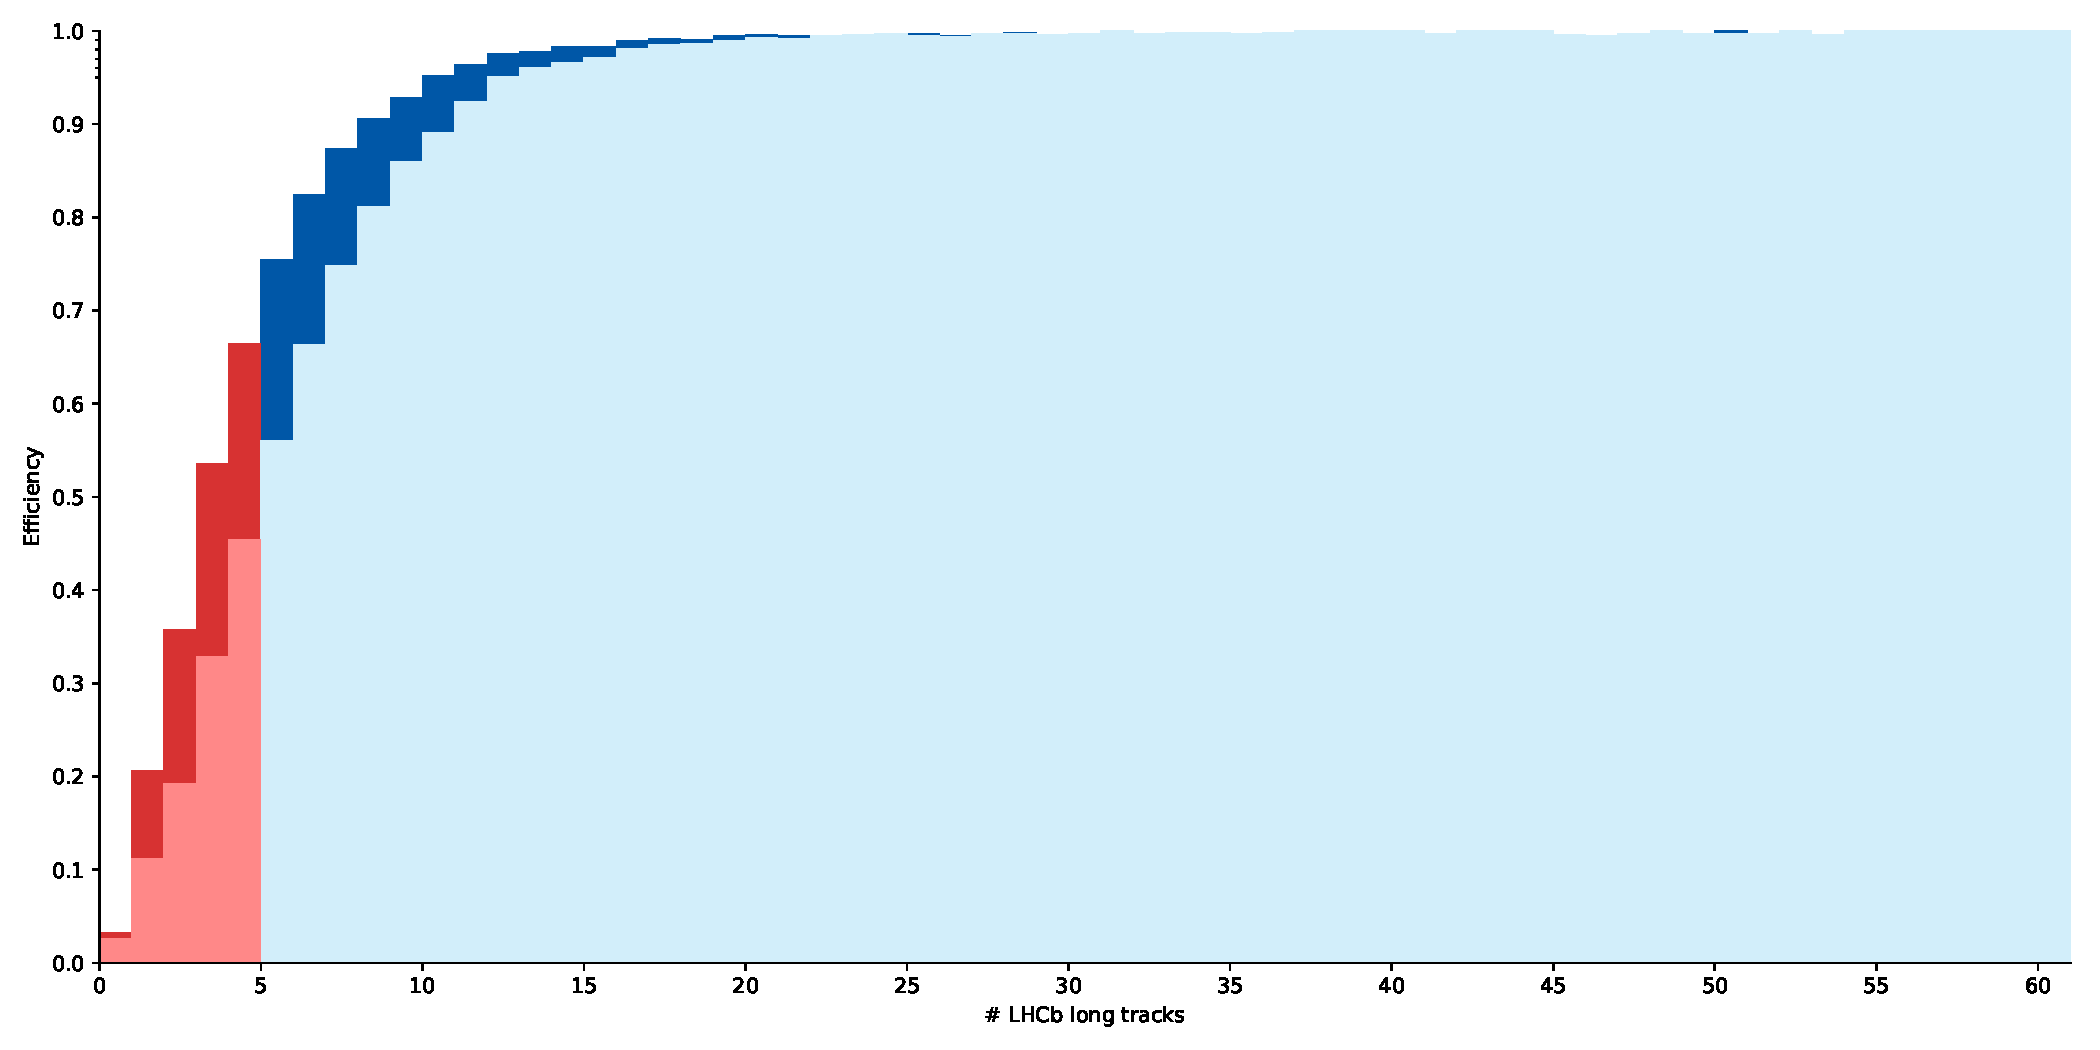
\includegraphics[width=14.7cm]{images/effntracks_bg.pdf}};
    \end{tikzpicture}
\begin{columns}
\column{.25\textwidth}
\column{.65\textwidth}
\setstretch{0.92}
\vskip -1.75em
    \begin{itemize}
    \setlength\itemsep{0.25em}
        \item [\textcolor{lhcbRed}{\textbullet}] \color{lhcbRed}
          Proof-of-Principle established:
          \color{lhcbBlue}
          a hybrid ML algorithm using a 1-dimensional KDE processed by a 5-layer CNN finds primary vertices with efficiencies and false positive rates similar to traditional algorithms.
        \item [\textcolor{lhcbRed}{\textbullet}] \color{lhcbRed} Efficiency is tunable; \color{lhcbBlue} increasing the efficiency also increases the false positive rate.
        \item [\textcolor{lhcbRed}{\textbullet}] \color{lhcbRed} Adding information
        should improve performance.
        \color{lhcbBlue}
        \begin{itemize}
            \item [\textcolor{lhcbBlue}
            {\textbullet} \color{lhcbBlue}] \color{lhcbBlue}
            can add KDE (x,y) information to algorithm
            \item [\color{lhcbBlue}{\textbullet} \color{lhcbBlue}]
            \color{lhcbBlue} can associate tracks to PV candidates, then iterate.
        \end{itemize}
        \item [\textcolor{lhcbRed}{\textbullet}] \color{lhcbRed} Next steps:
        \color{lhcbBlue}
        train with full LHCb MC and deploy inference engine in LHCb Hlt1 framework.
        \item [\textcolor{lhcbRed}{\textbullet}] \color{lhcbRed} Beyond LHCb
        \begin{itemize}
            \item [\color{lhcbBlue} {\textbullet}] \color{lhcbBlue}
                approach might work for ATLAS and CMS (in 2D?);
            \item [\color{lhcbBlue} {\textbullet}] \color{lhcbBlue} algorithm is an interesting ML laboratory.
        \end{itemize}
    \end{itemize}
\column{.1\textwidth}
\end{columns}
\end{frame}


\subsection{Final words}
\begin{frame}{Final words}

    \begin{block}{Thanks to support from:}
    \begin{itemize}
        \item \href{https://www.nsf.gov/awardsearch/showAward?AWD_ID=1836650}{OAC-1836650: IRIS-HEP}
        \item \href{https://www.nsf.gov/awardsearch/showAward?AWD_ID=1740102}{OAC-1740102: SI2:SSE}
        \item \href{https://www.nsf.gov/awardsearch/showAward?AWD_ID=1739772}{OAC-1739772: SI2:SSE}
    \end{itemize}
    \end{block}
\end{frame}



%%%%%%%%%%%%%%%%%%%%%%%%%%%%%%%%%%%%%%%%%%%%%%%%%%%%%%%%%%%%%%%%%%%%%%%%%%%%%%%

\backupbegin
\section{Backup}

\subsection{Predictions with targets}
\begin{frame}{Compare predictions with targets (3 convolutional layers)}
  \begin{columns}[c]
    \column{.5\textwidth}
        \begin{center}
            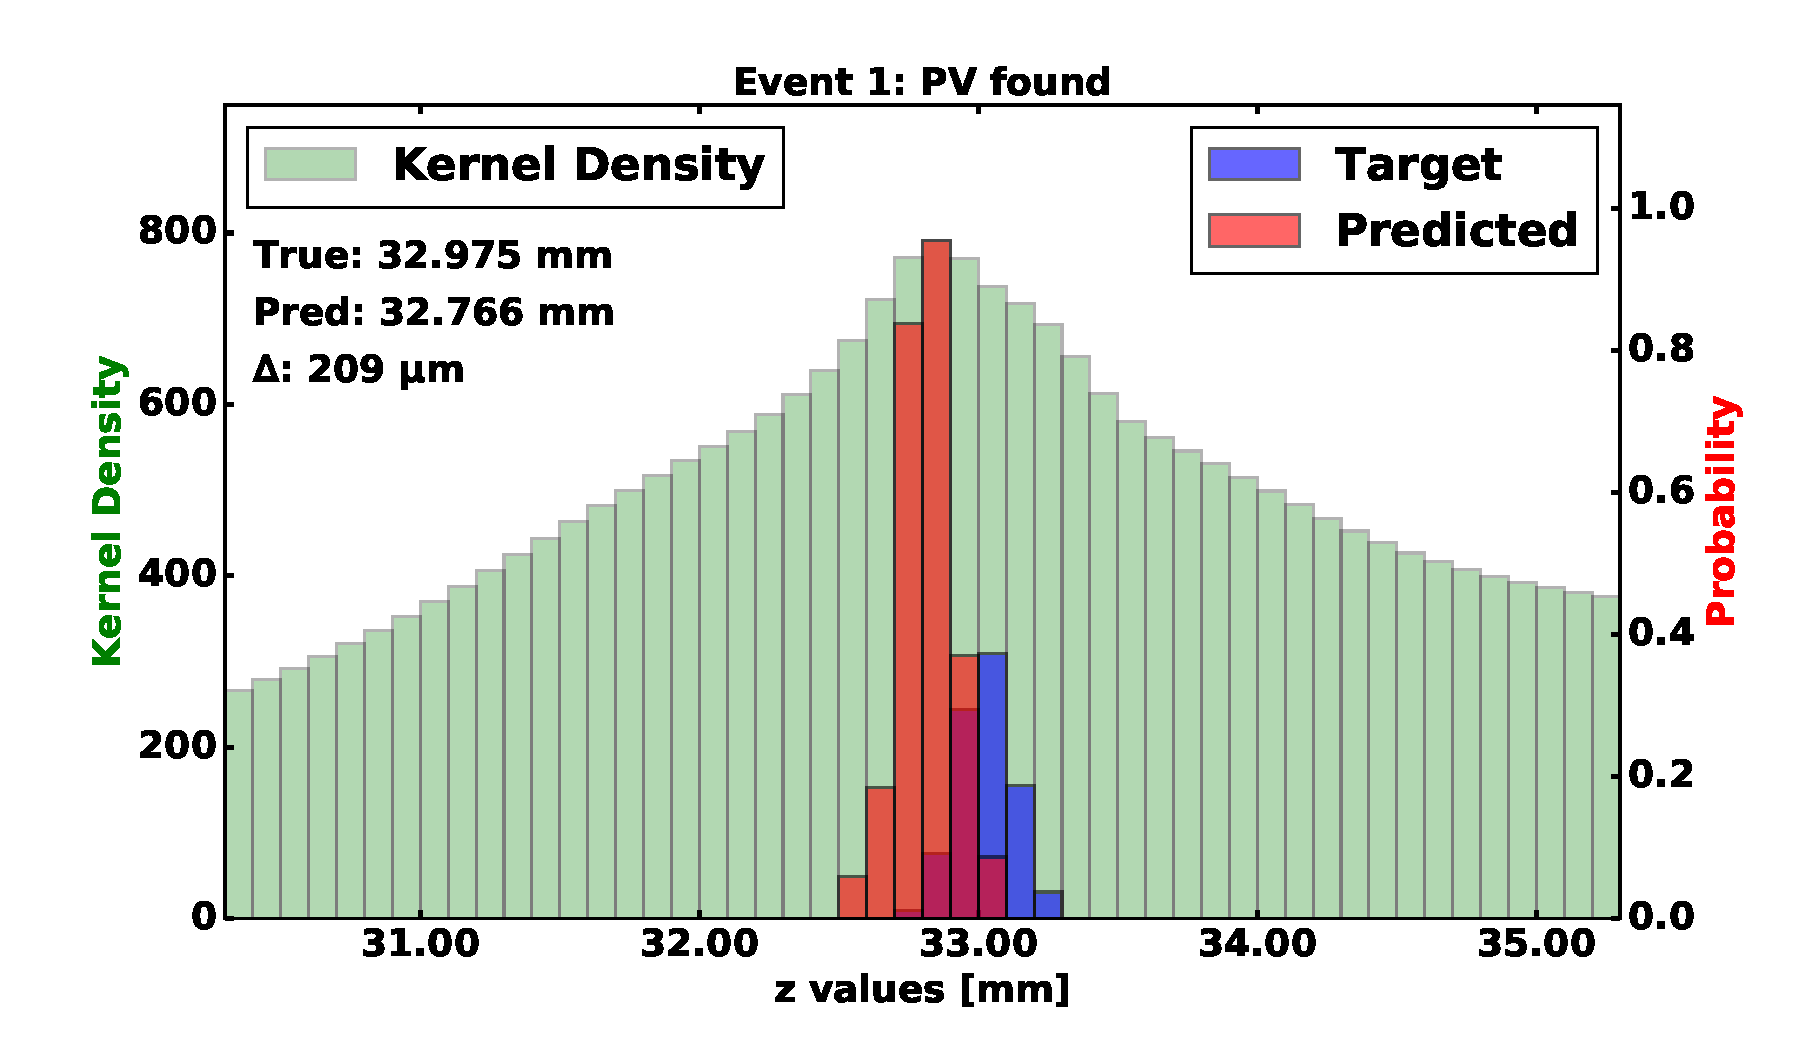
\includegraphics[width=1\textwidth,height=0.45\textwidth, trim=18 0 18 0]{images/120000_3layer_04.pdf}

            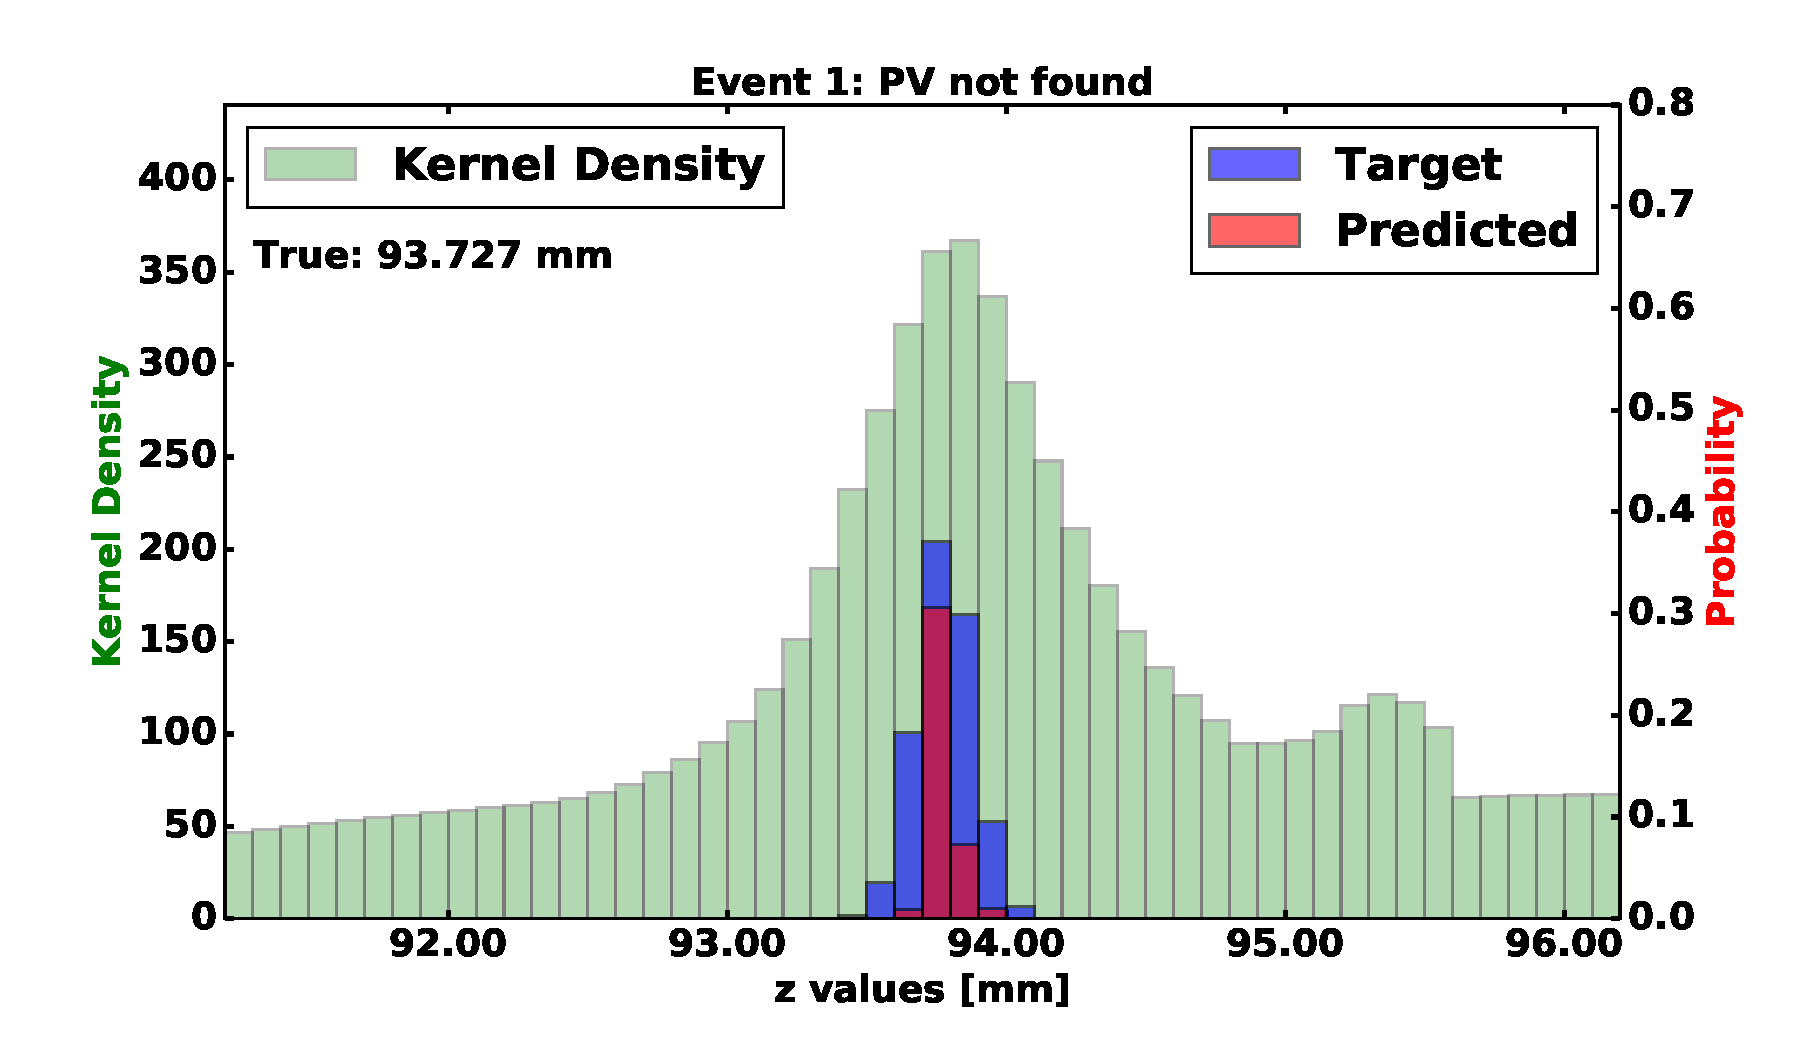
\includegraphics[width=1\textwidth, height=0.45\textwidth,trim=18 0 18 0]{images/120000_3layer_05.pdf}

        \end{center}
    \column{.5\textwidth}
        \begin{center}
           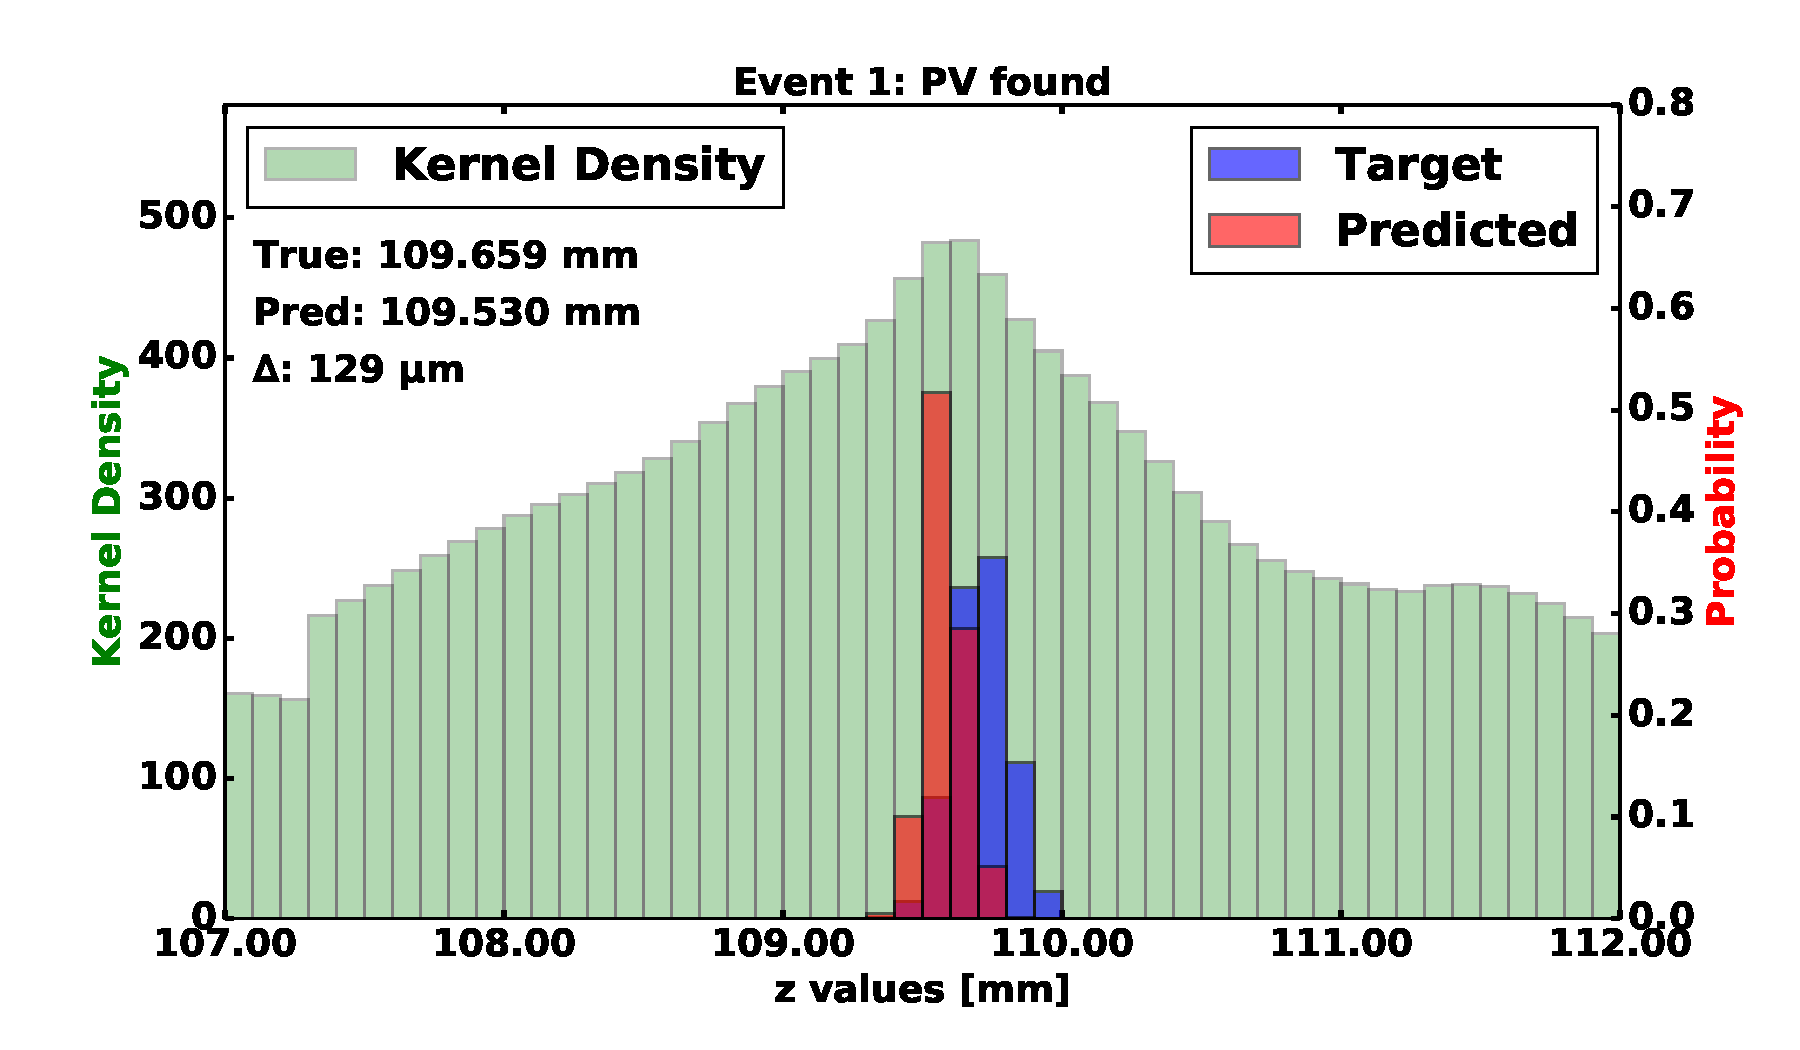
\includegraphics[width=1\textwidth, height=0.45\textwidth, trim=18 0 18 0]{images/120000_3layer_06.pdf}

           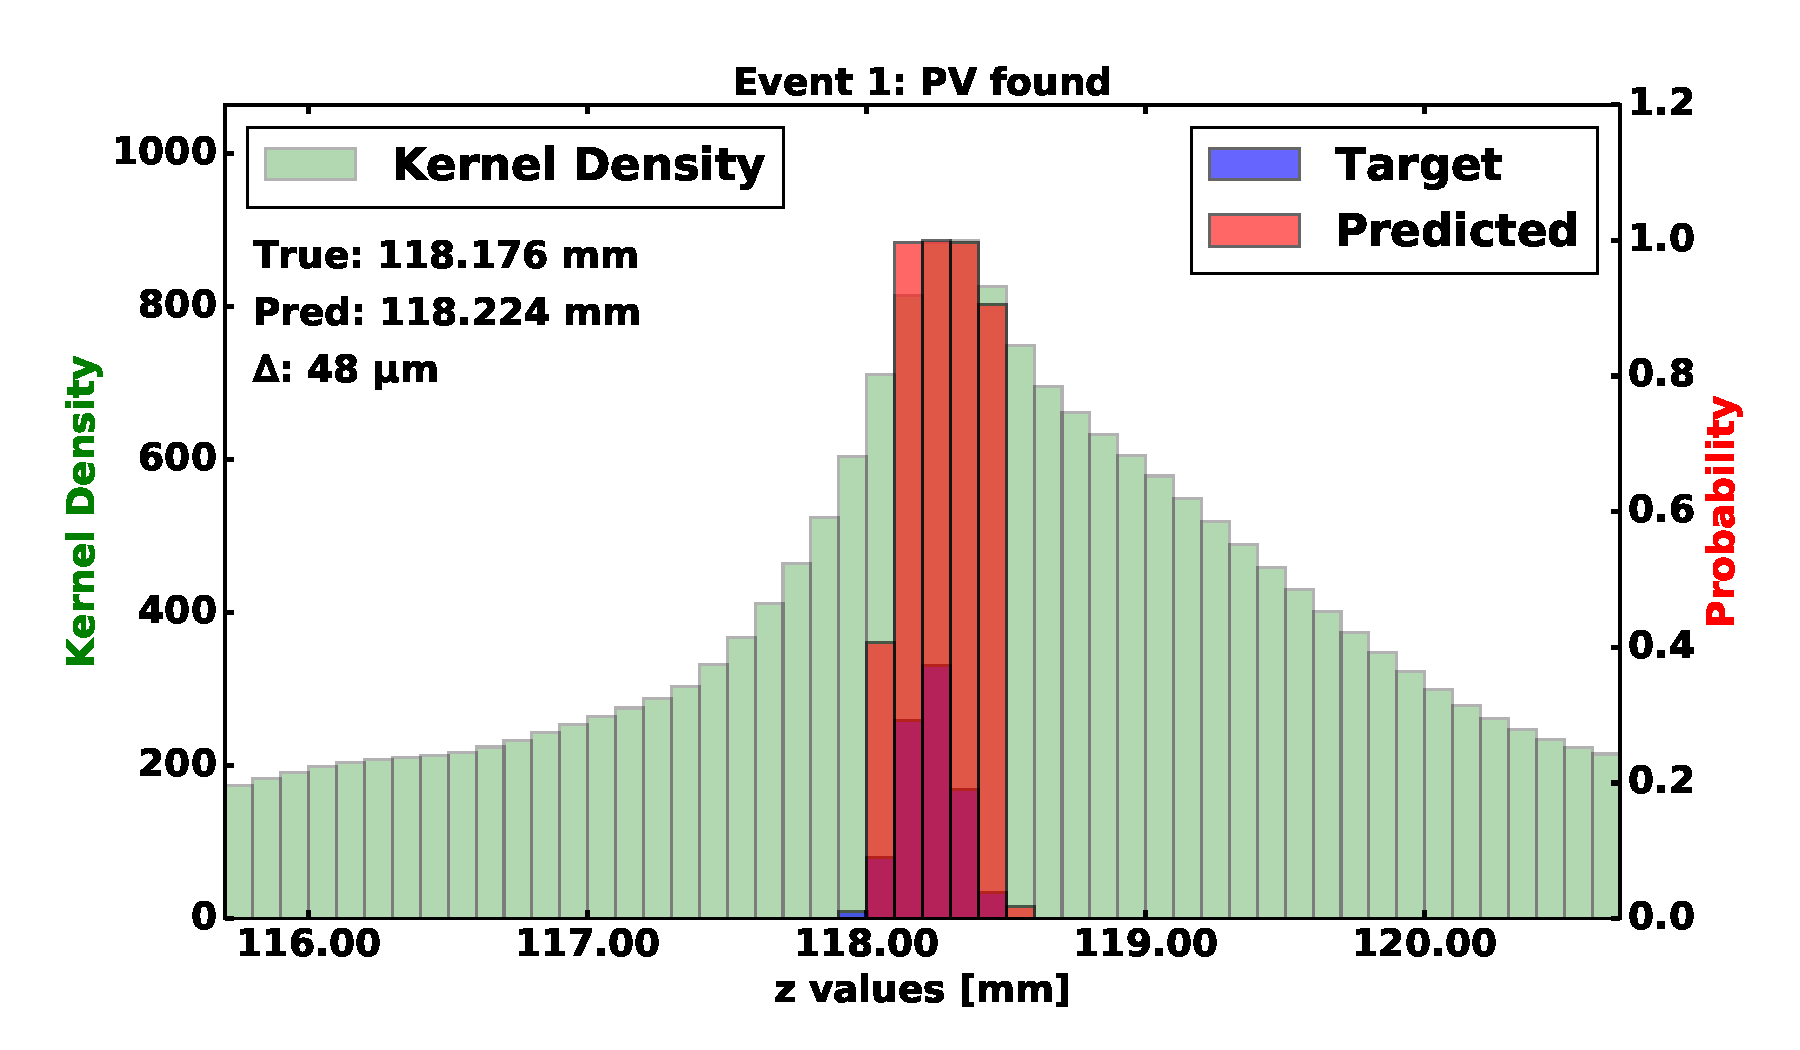
\includegraphics[width=1\textwidth, height=0.45\textwidth, trim=18 0 18 0]{images/120000_3layer_07.pdf}
       \end{center}
  \end{columns}
\end{frame}

\begin{frame}{Compare predictions with targets (3 convolutional layers)}
  \begin{columns}[c]
    \column{.5\textwidth}
        \begin{center}
            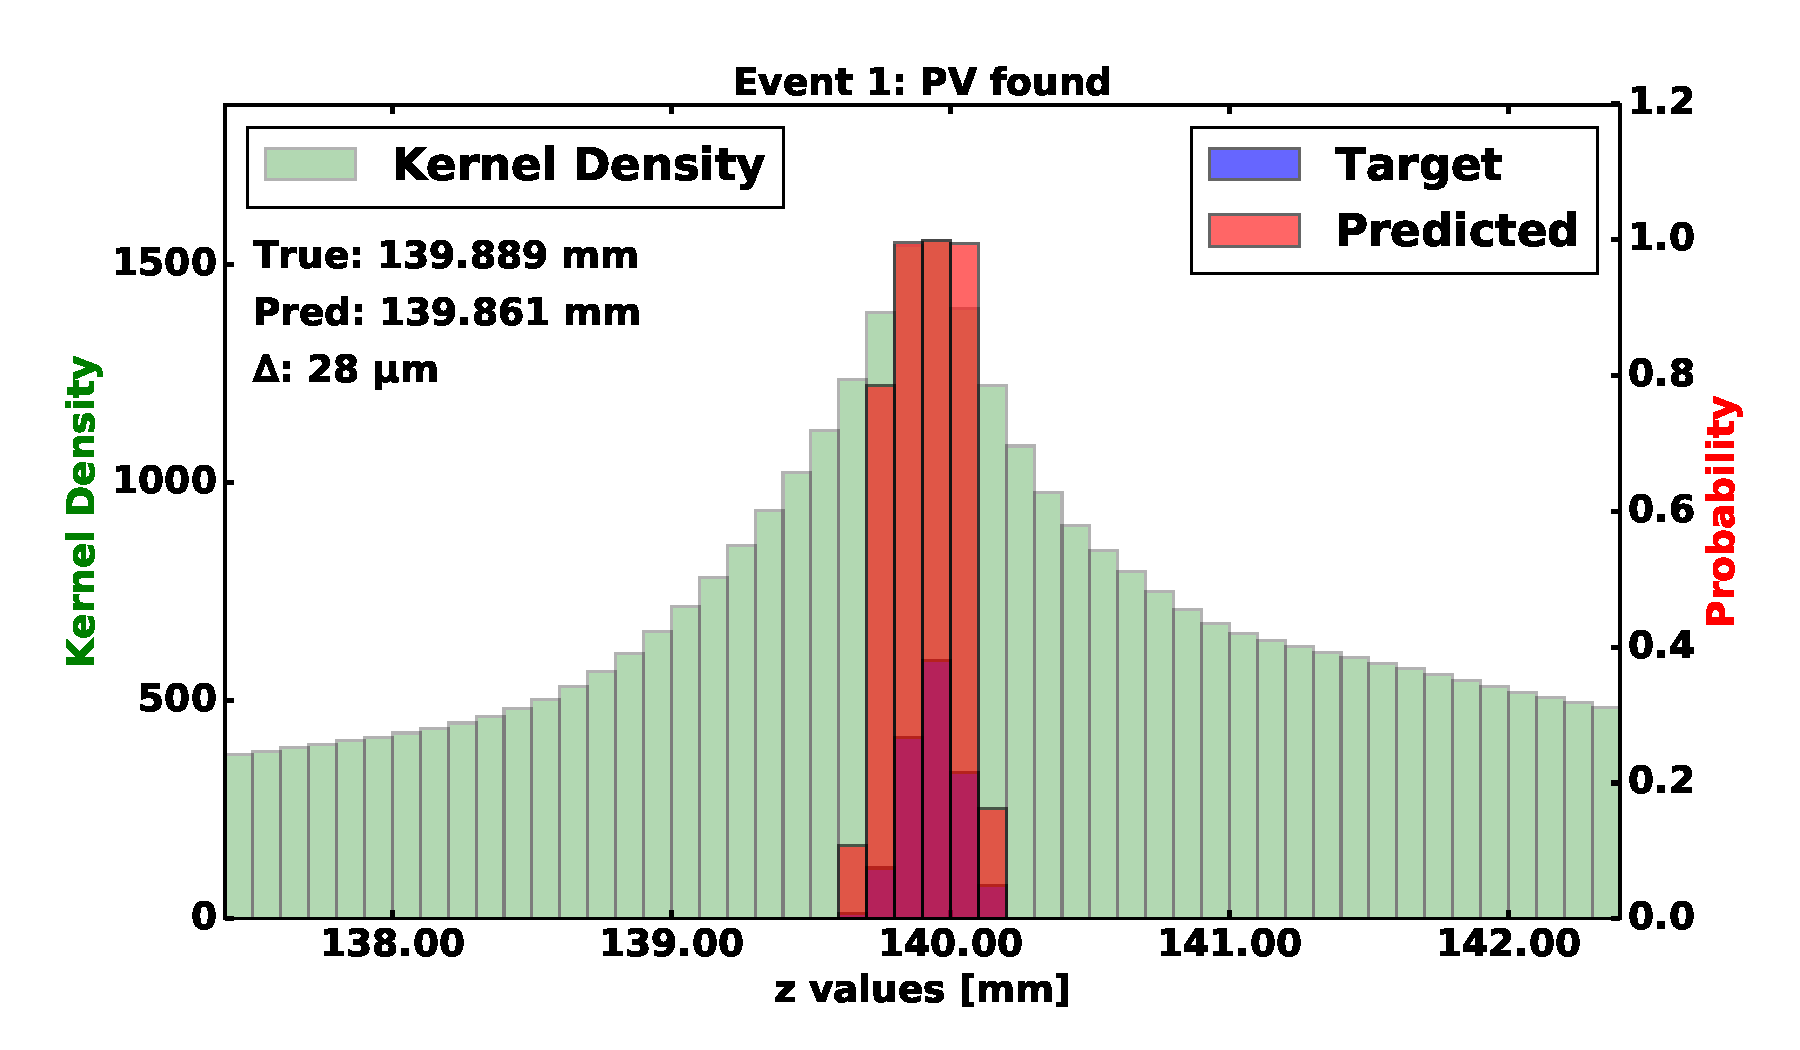
\includegraphics[width=1\textwidth,height=0.45\textwidth, trim=18 0 18 0]{images/120000_3layer_08.pdf}

            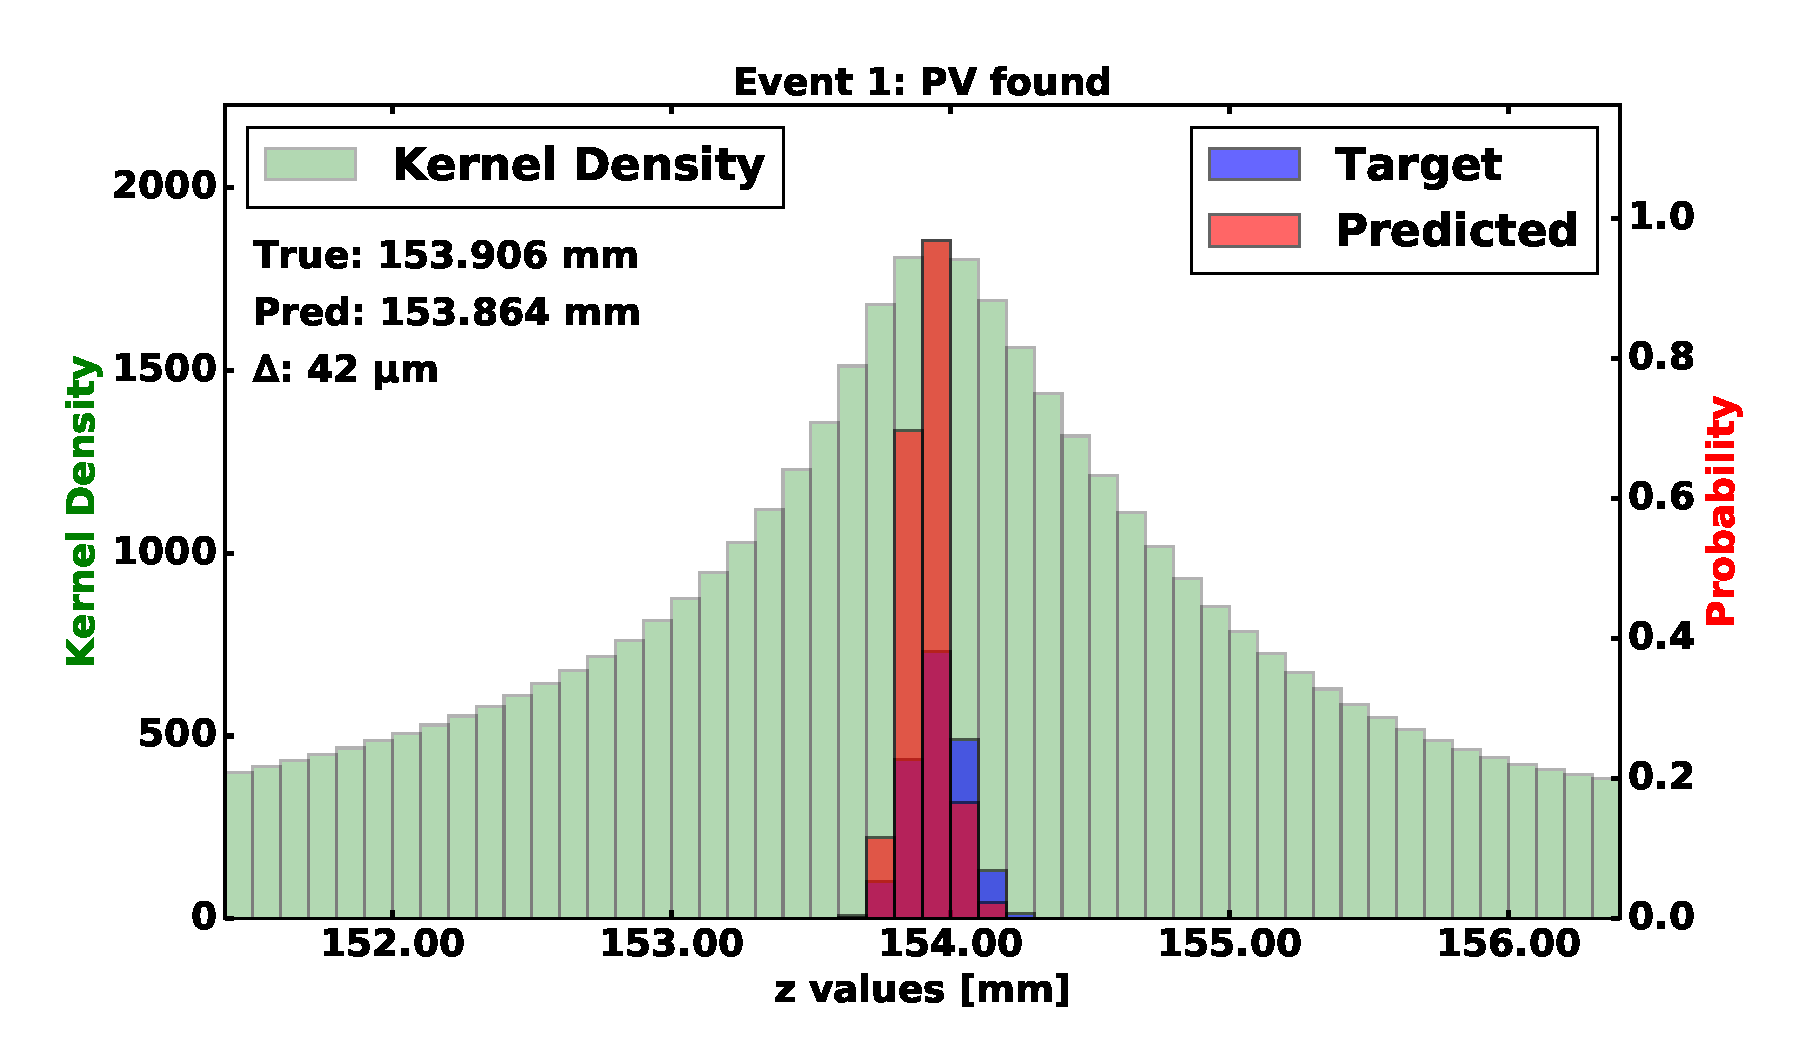
\includegraphics[width=1\textwidth, height=0.45\textwidth,trim=18 0 18 0]{images/120000_3layer_09.pdf}

        \end{center}
    \column{.5\textwidth}
        \begin{center}
           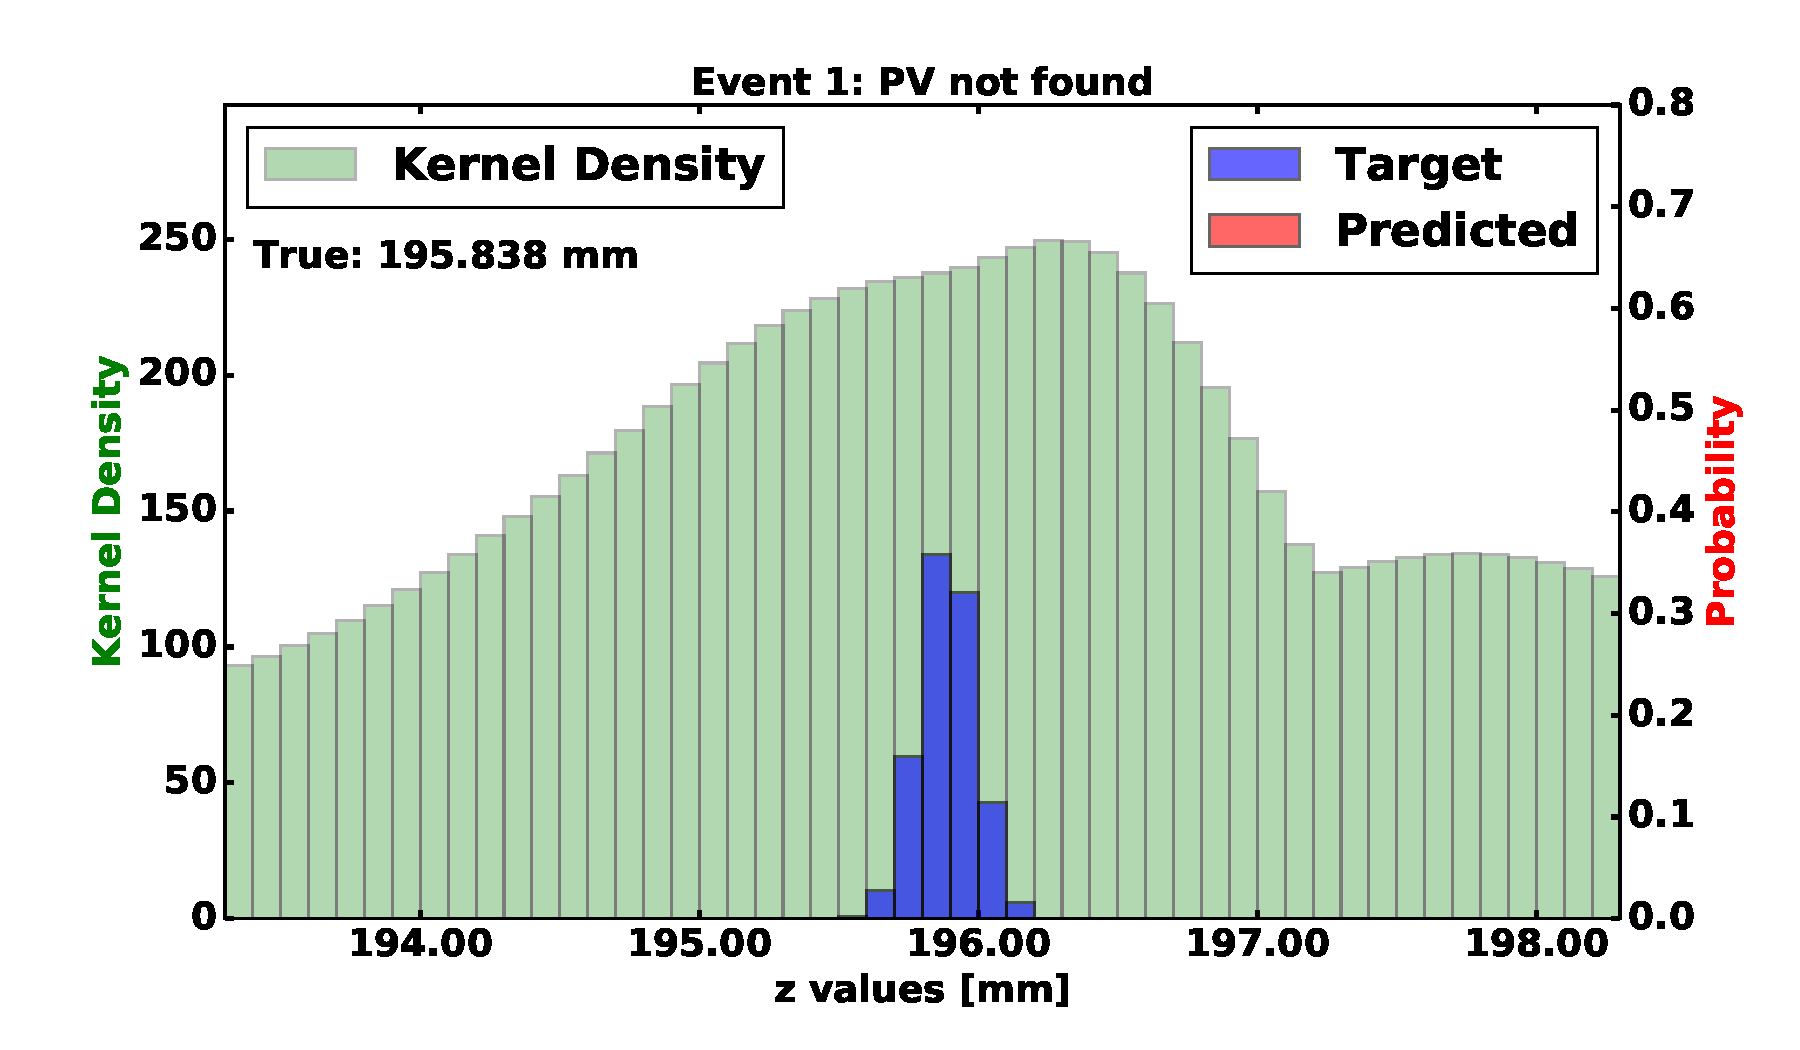
\includegraphics[width=1\textwidth, height=0.45\textwidth, trim=18 0 18 0]{images/120000_3layer_10.pdf}

           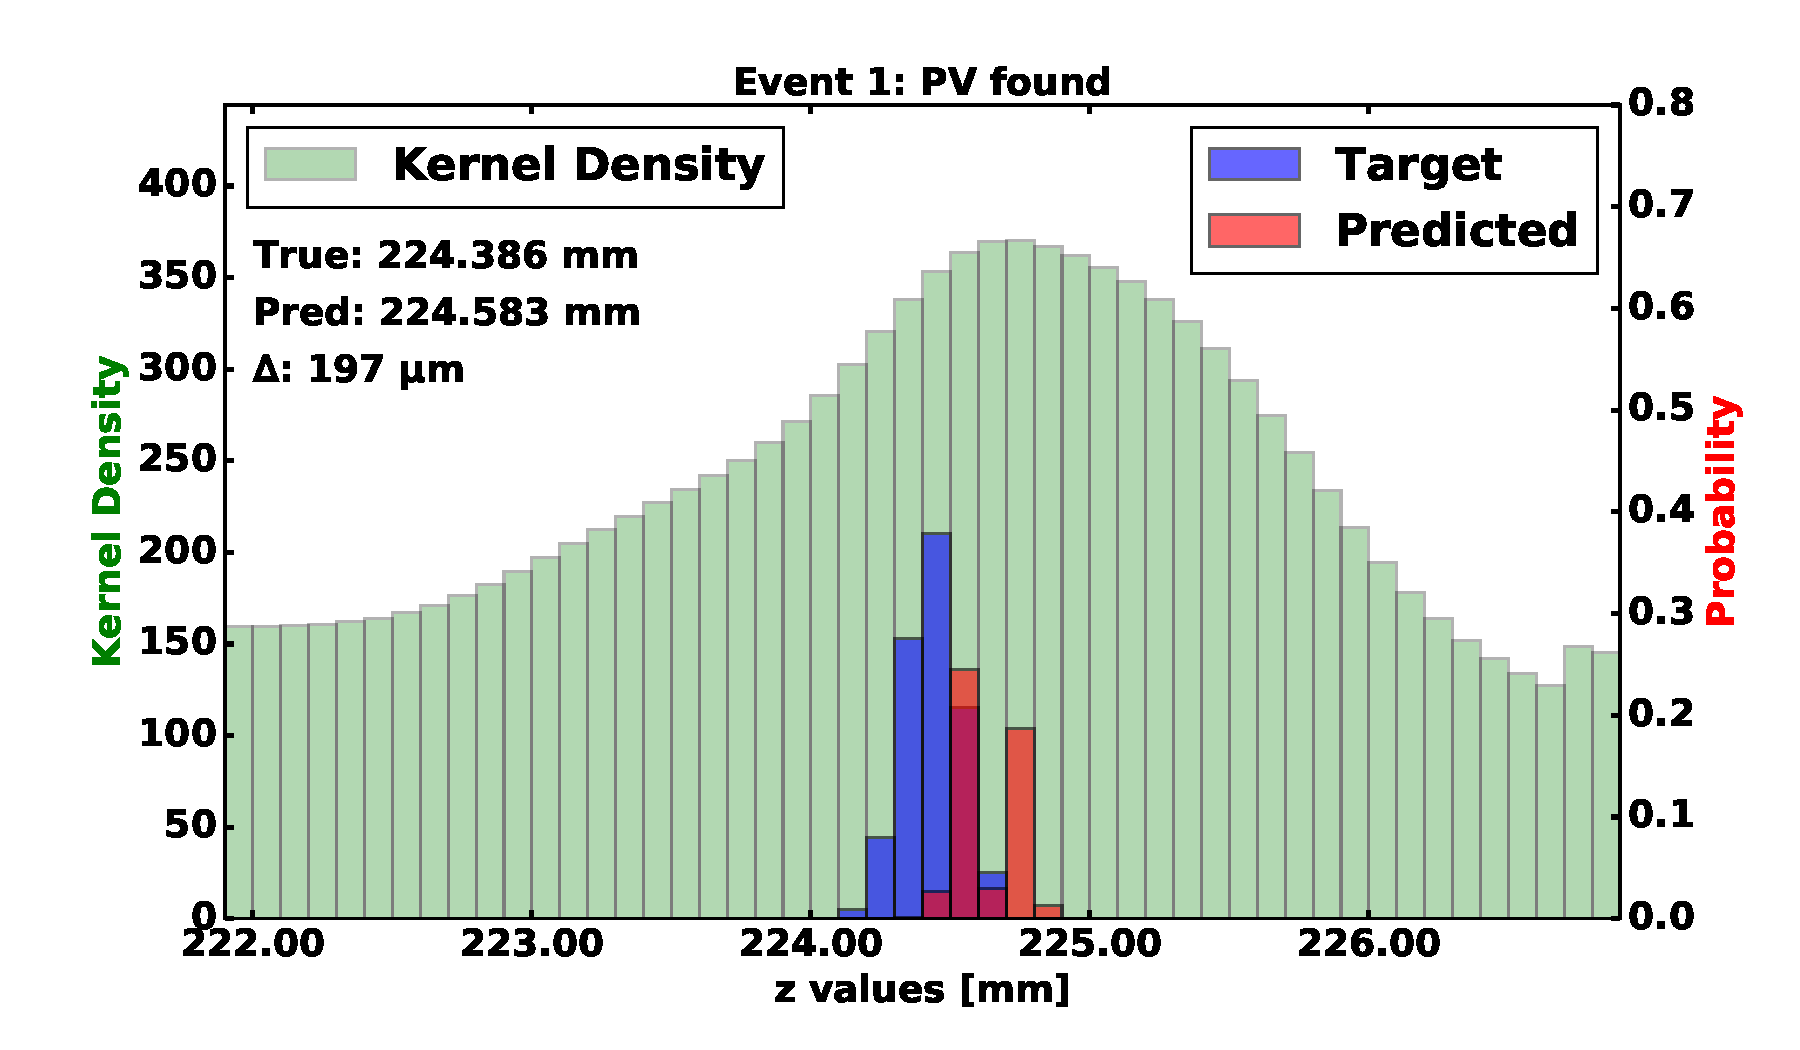
\includegraphics[width=1\textwidth, height=0.45\textwidth, trim=18 0 18 0]{images/120000_3layer_11.pdf}
       \end{center}
  \end{columns}
\end{frame}


\subsection{More predictions with targets}
\begin{frame}{More predictions with targets (1)}
  \begin{columns}[c]
    \column{.5\textwidth}
        \begin{center}
           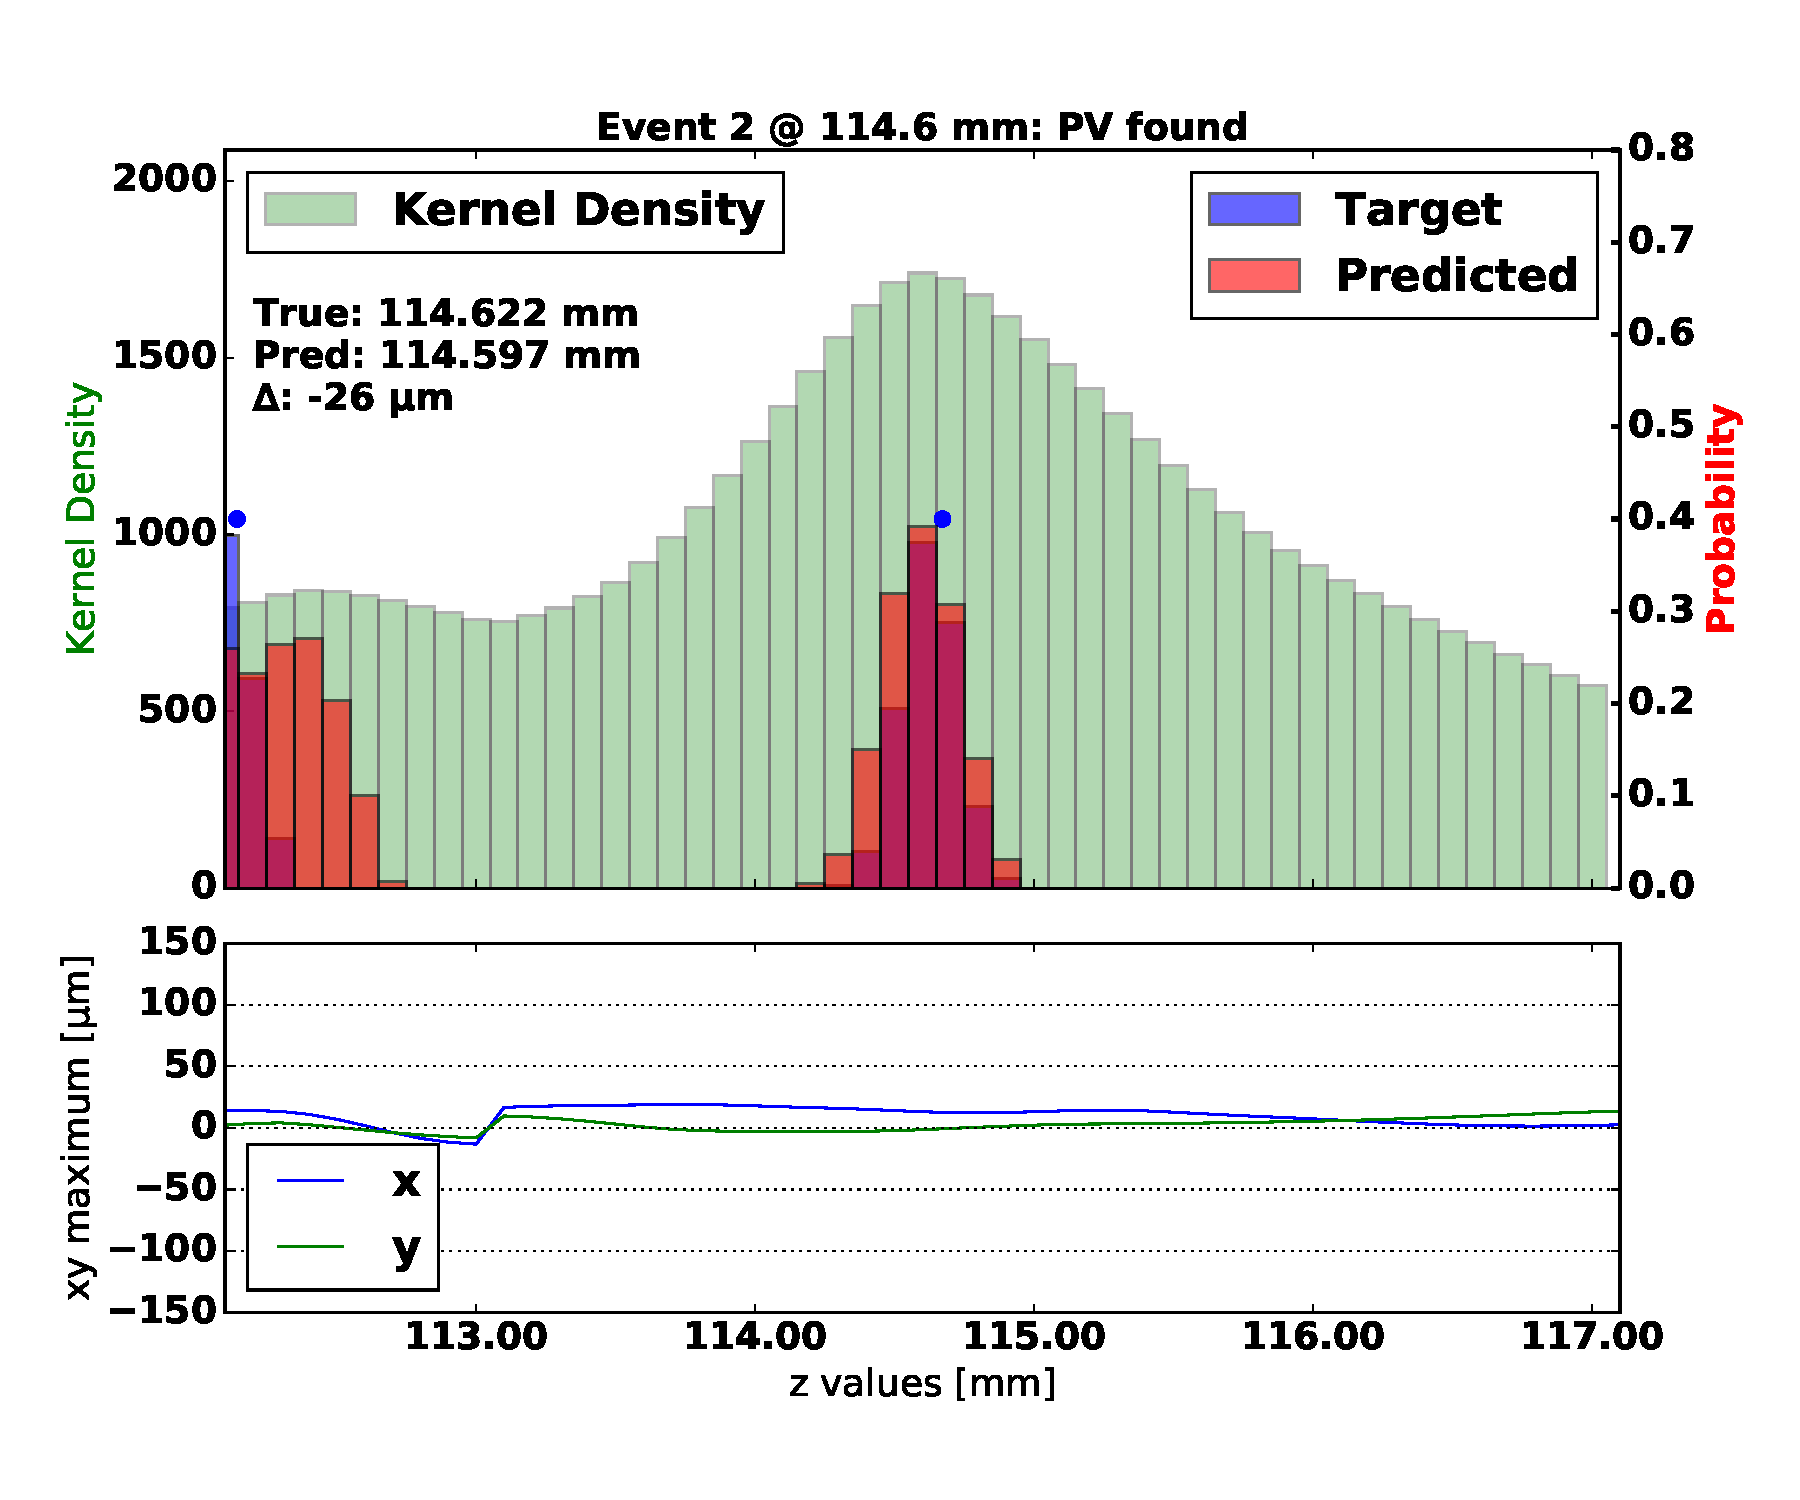
\includegraphics[width=1\textwidth, trim=60 0 60 0]{images/07Jan19_AltCNN4Layer_D35_sp_12.pdf}
       \end{center}
   \column{.5\textwidth}
       \begin{center}
           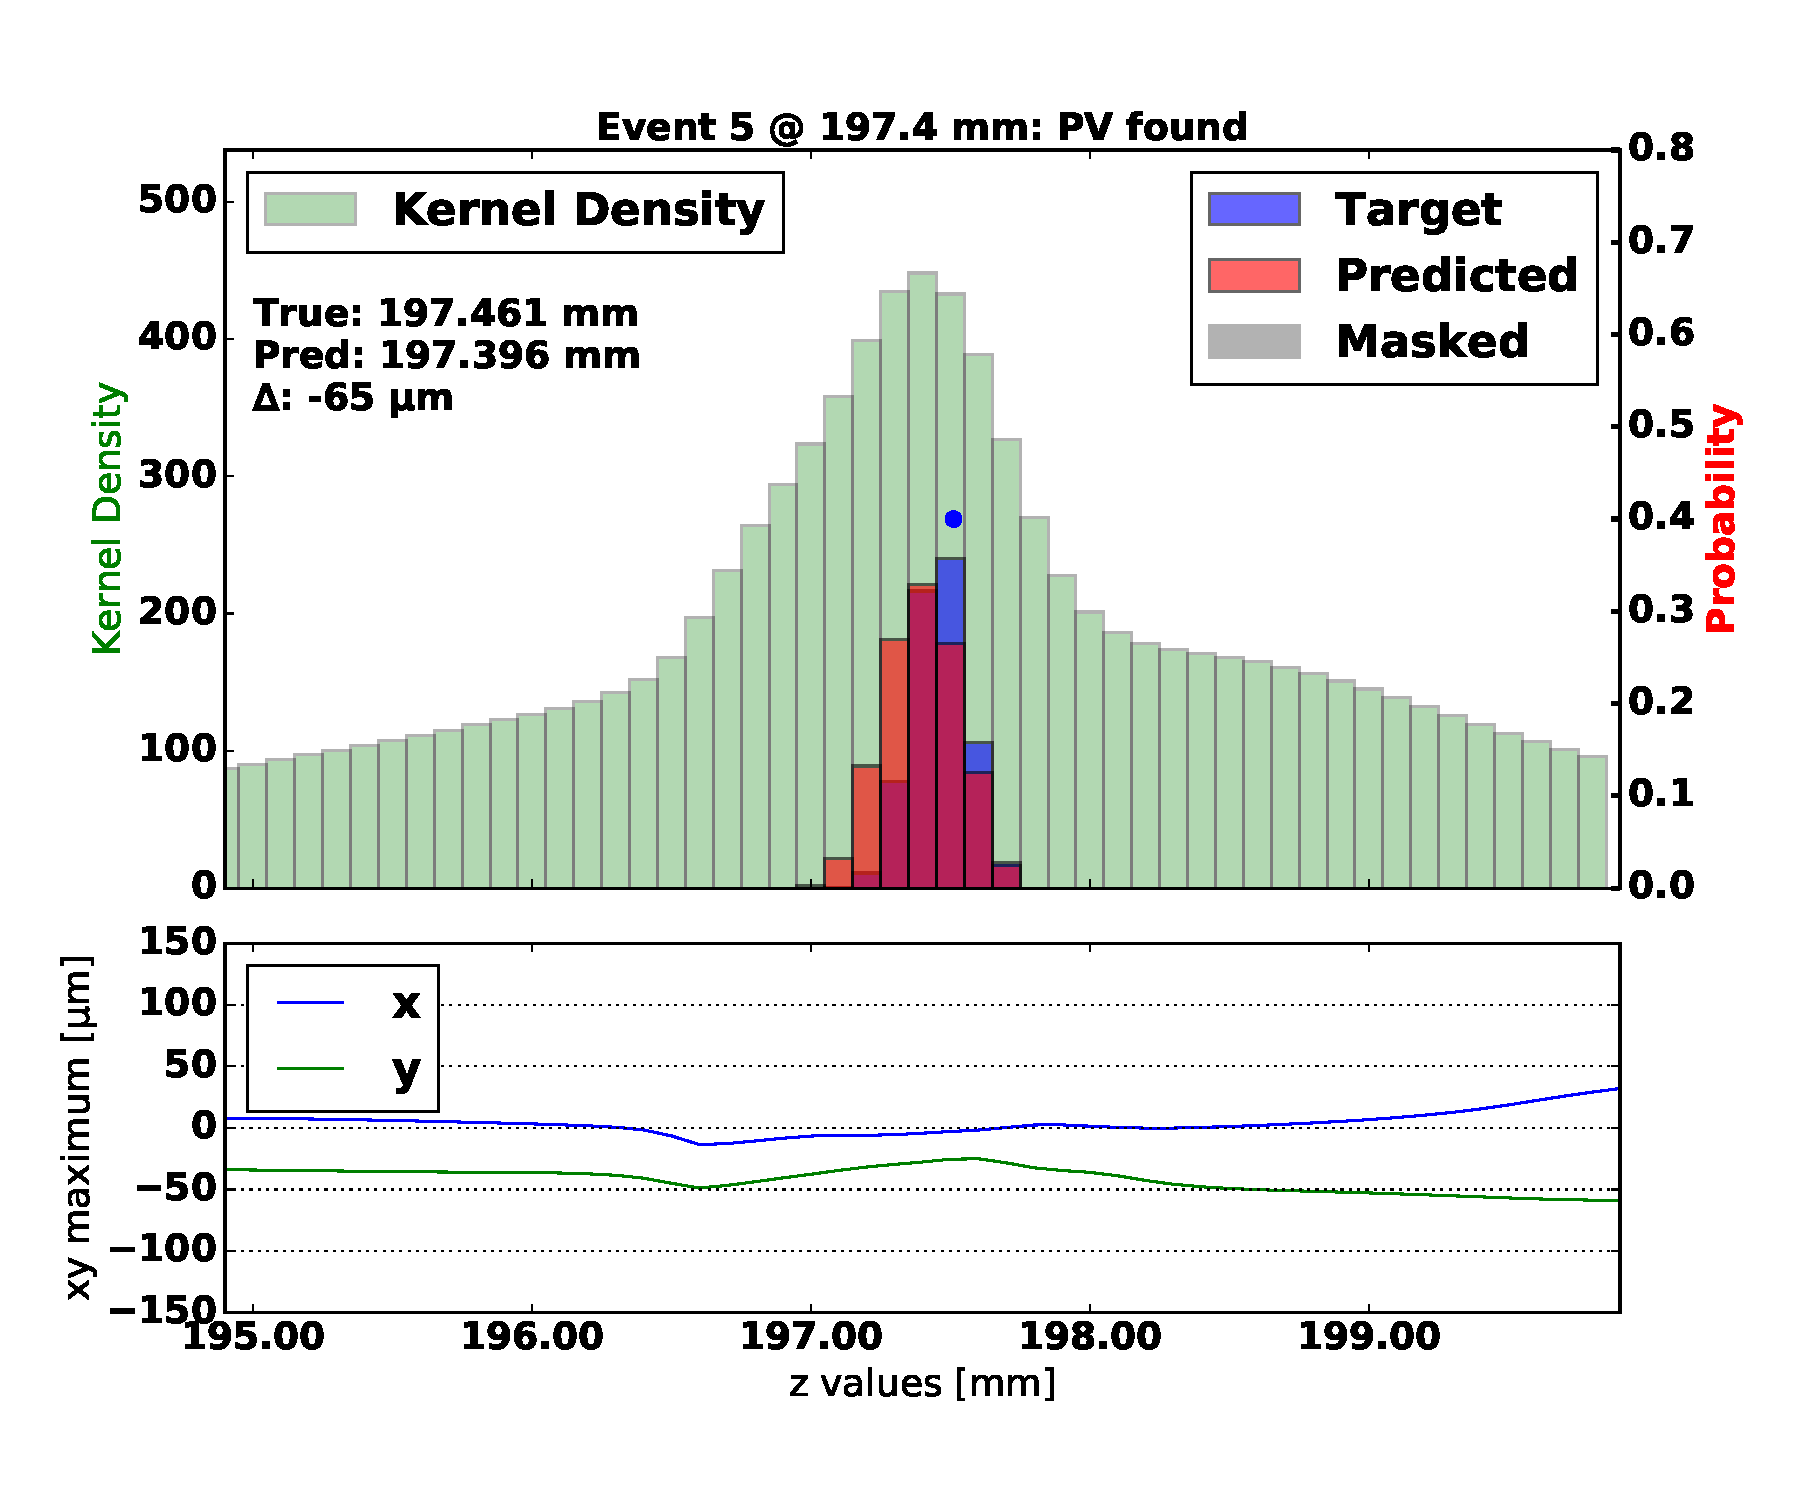
\includegraphics[width=1\textwidth, trim=60 0 60 0]{images/07Jan19_AltCNN4Layer_D35_sp_30.pdf}
       \end{center}
  \end{columns}
\end{frame}

\begin{frame}{More predictions with targets (2)}
  \begin{columns}[c]
    \column{.5\textwidth}
        \begin{center}
           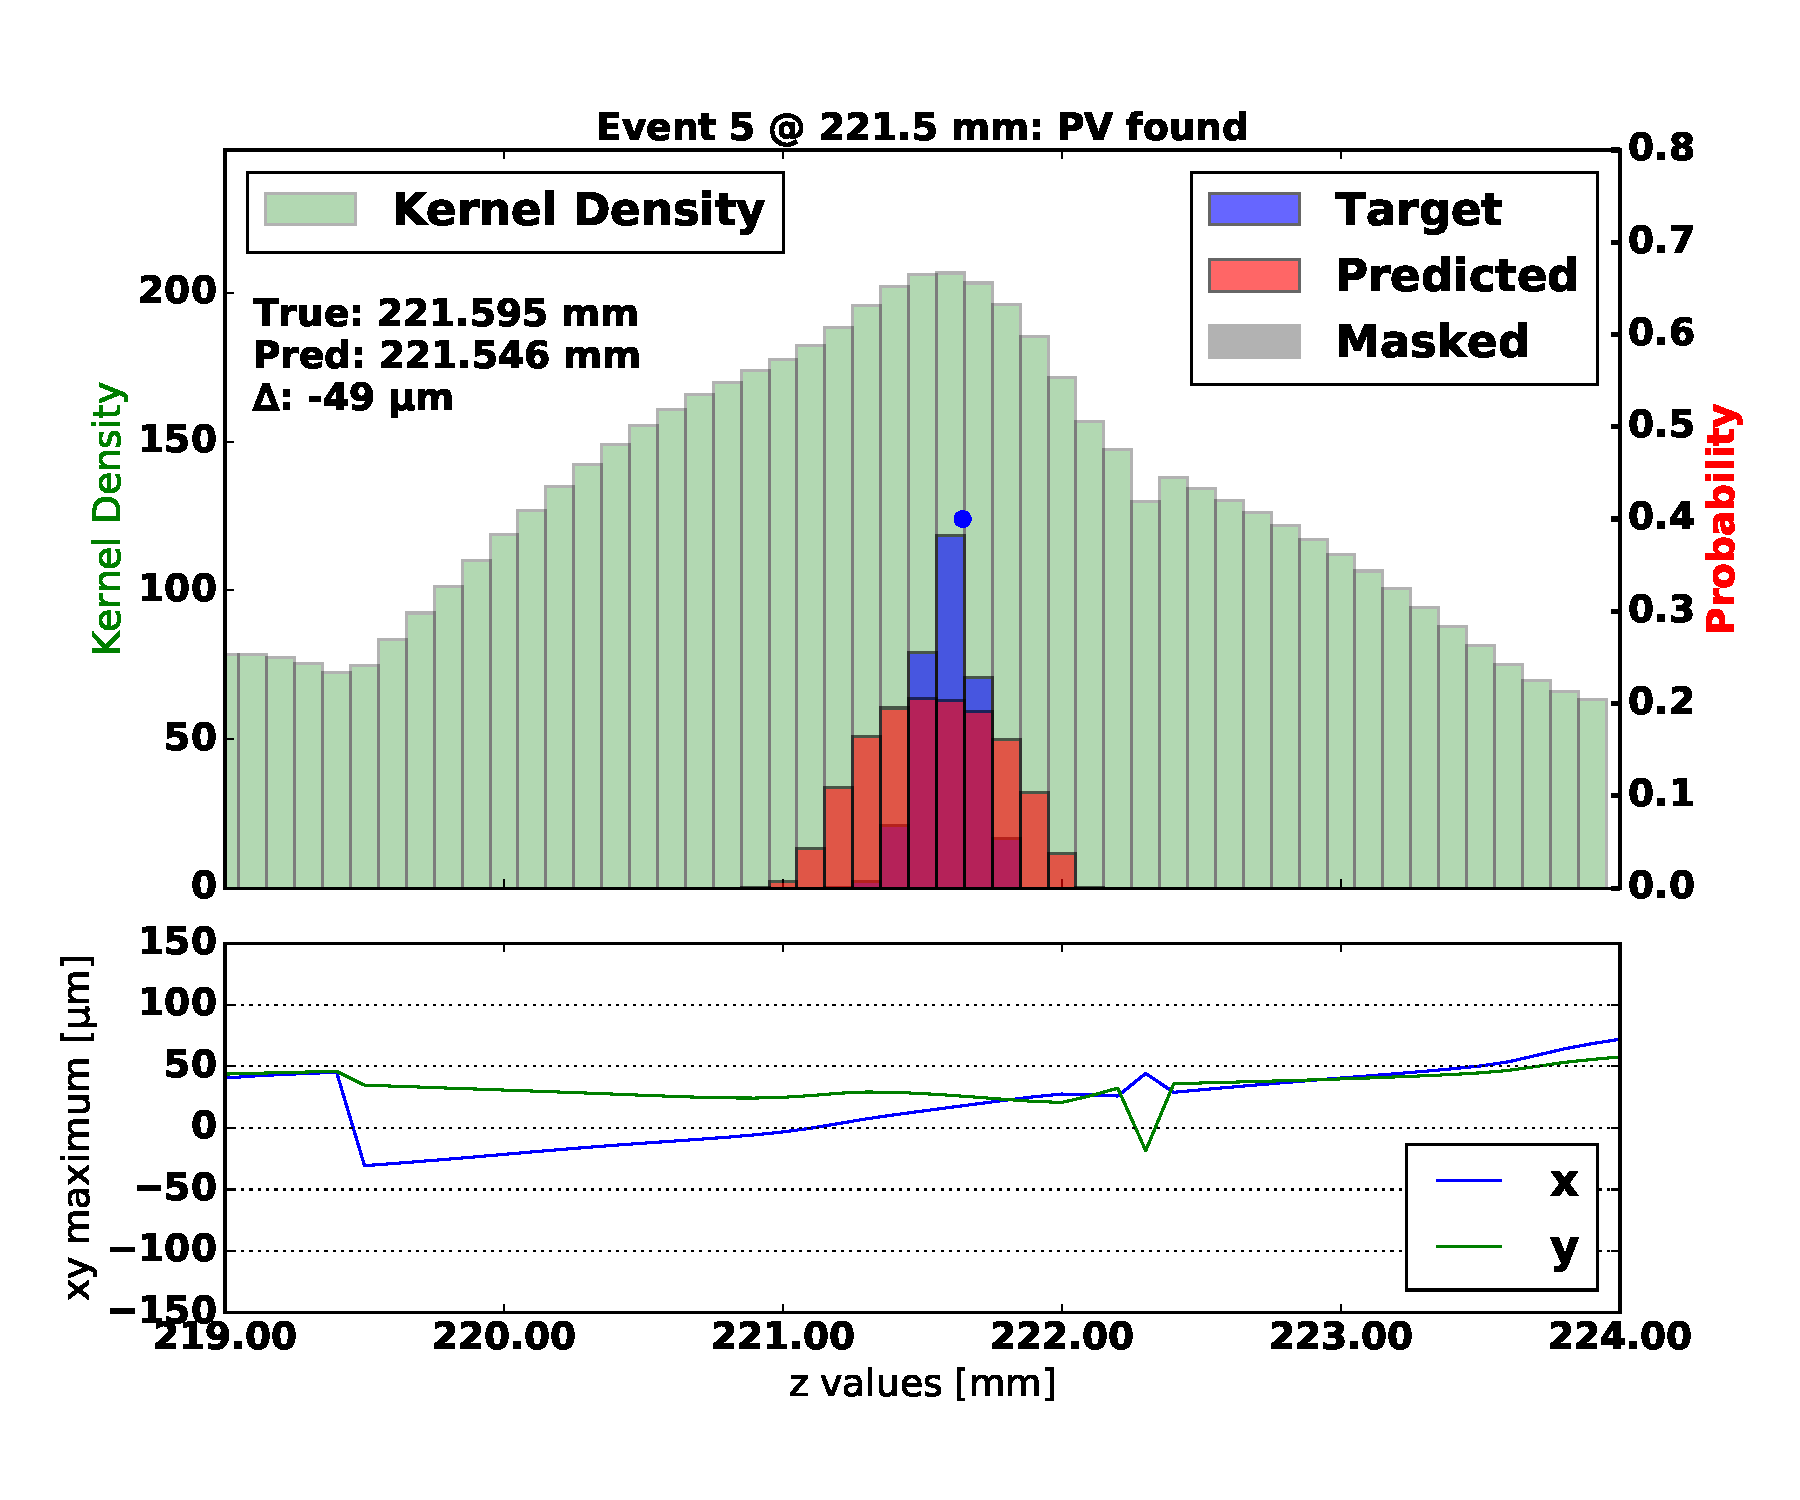
\includegraphics[width=1\textwidth, trim=60 0 60 0]{images/07Jan19_AltCNN4Layer_D35_sp_31.pdf}
        \end{center}
    \column{.5\textwidth}
        \begin{center}
           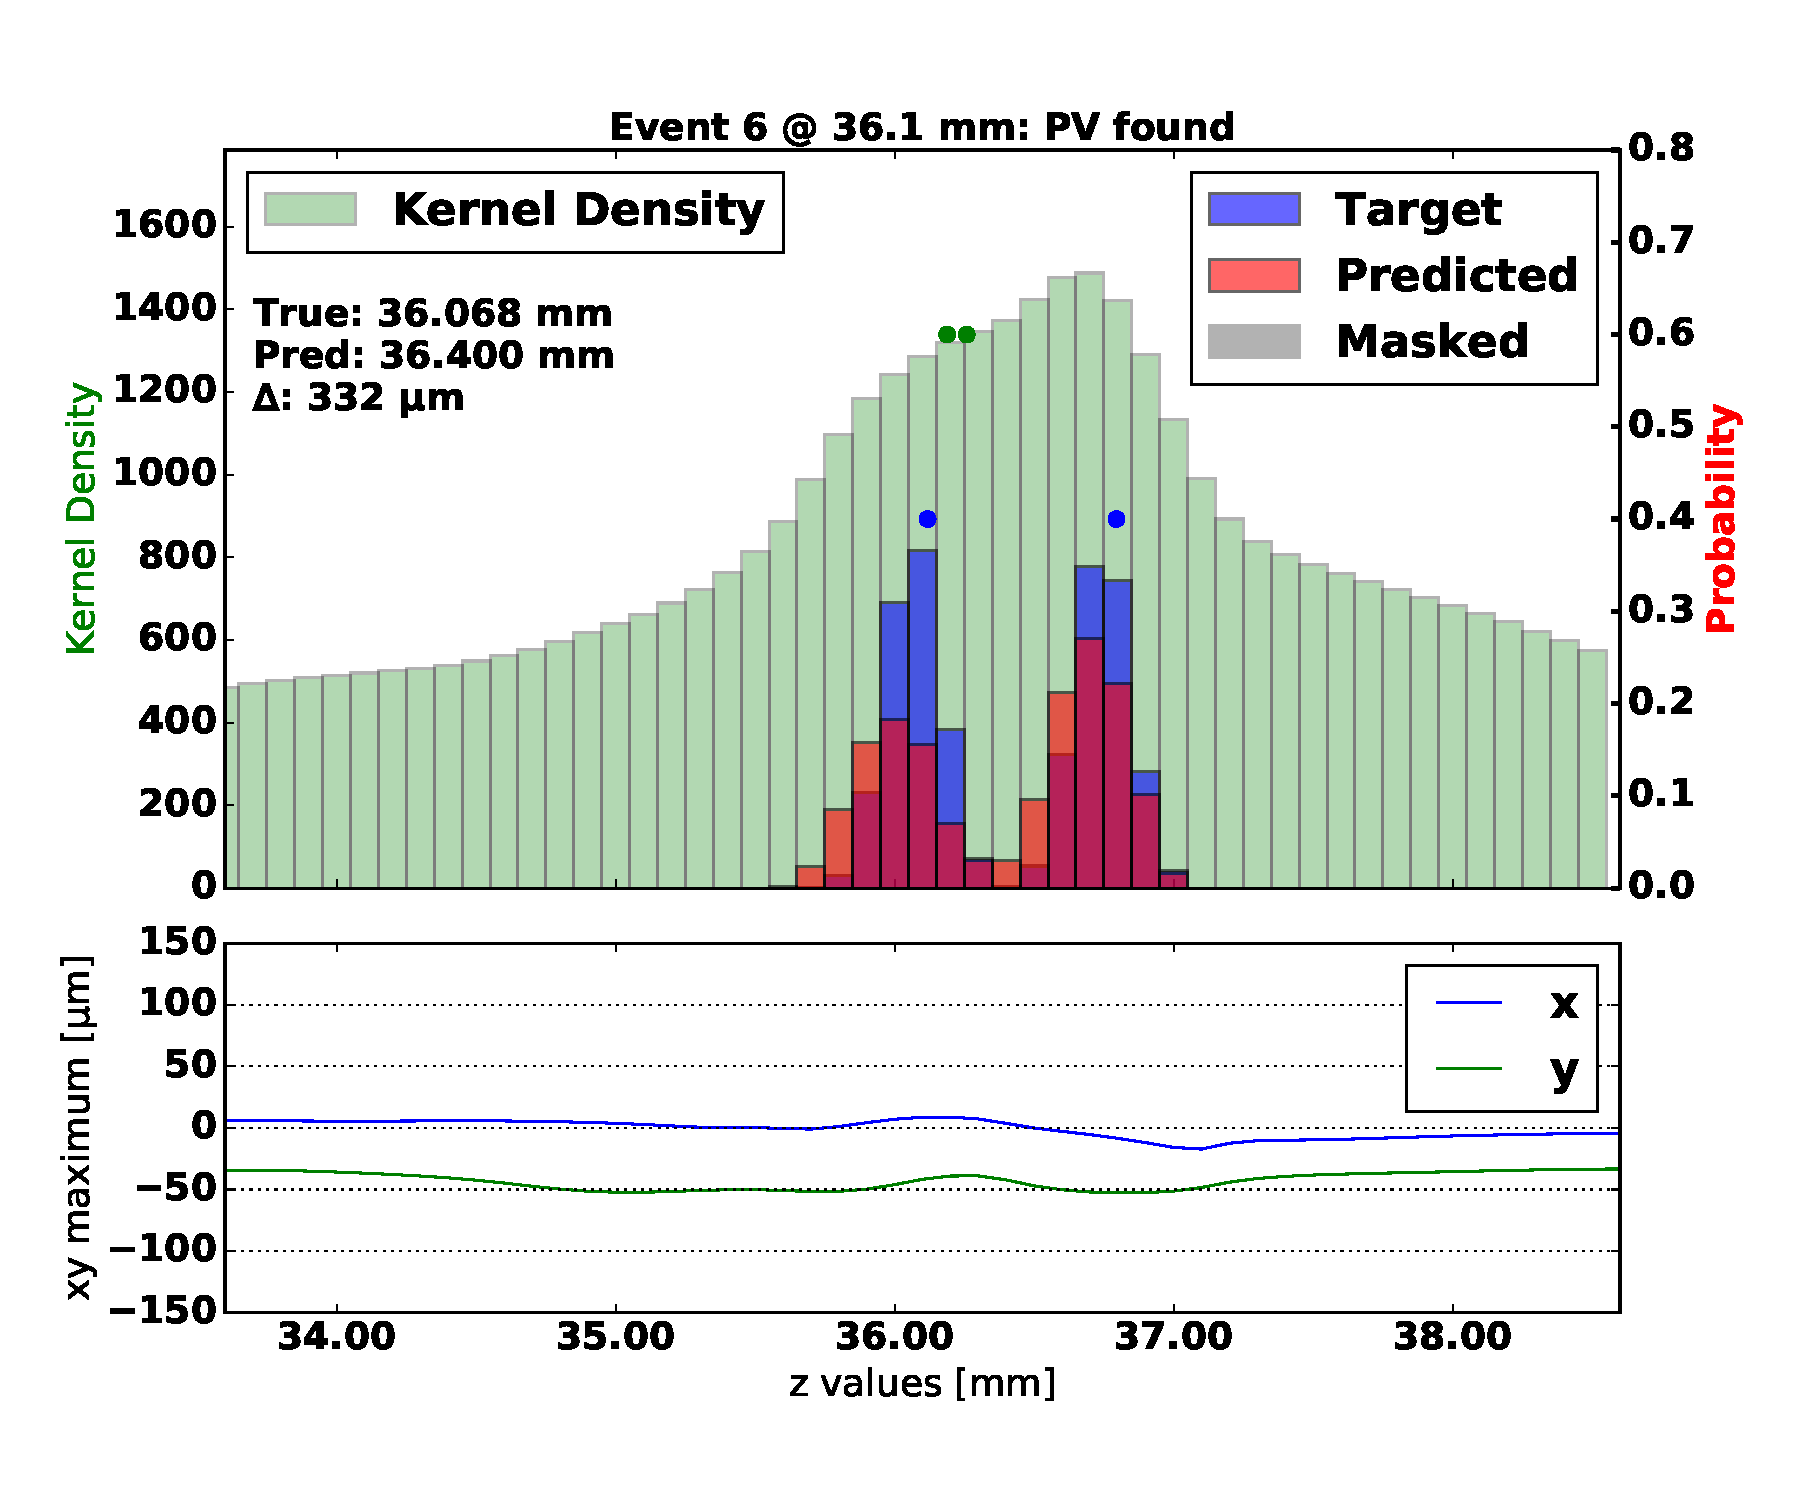
\includegraphics[width=1\textwidth, trim=60 0 60 0]{images/07Jan19_AltCNN4Layer_D35_sp_32.pdf}
       \end{center}
  \end{columns}
\end{frame}


\begin{frame}{More predictions with targets (3)}
  \begin{columns}[c]
    \column{.5\textwidth}
        \begin{center}
           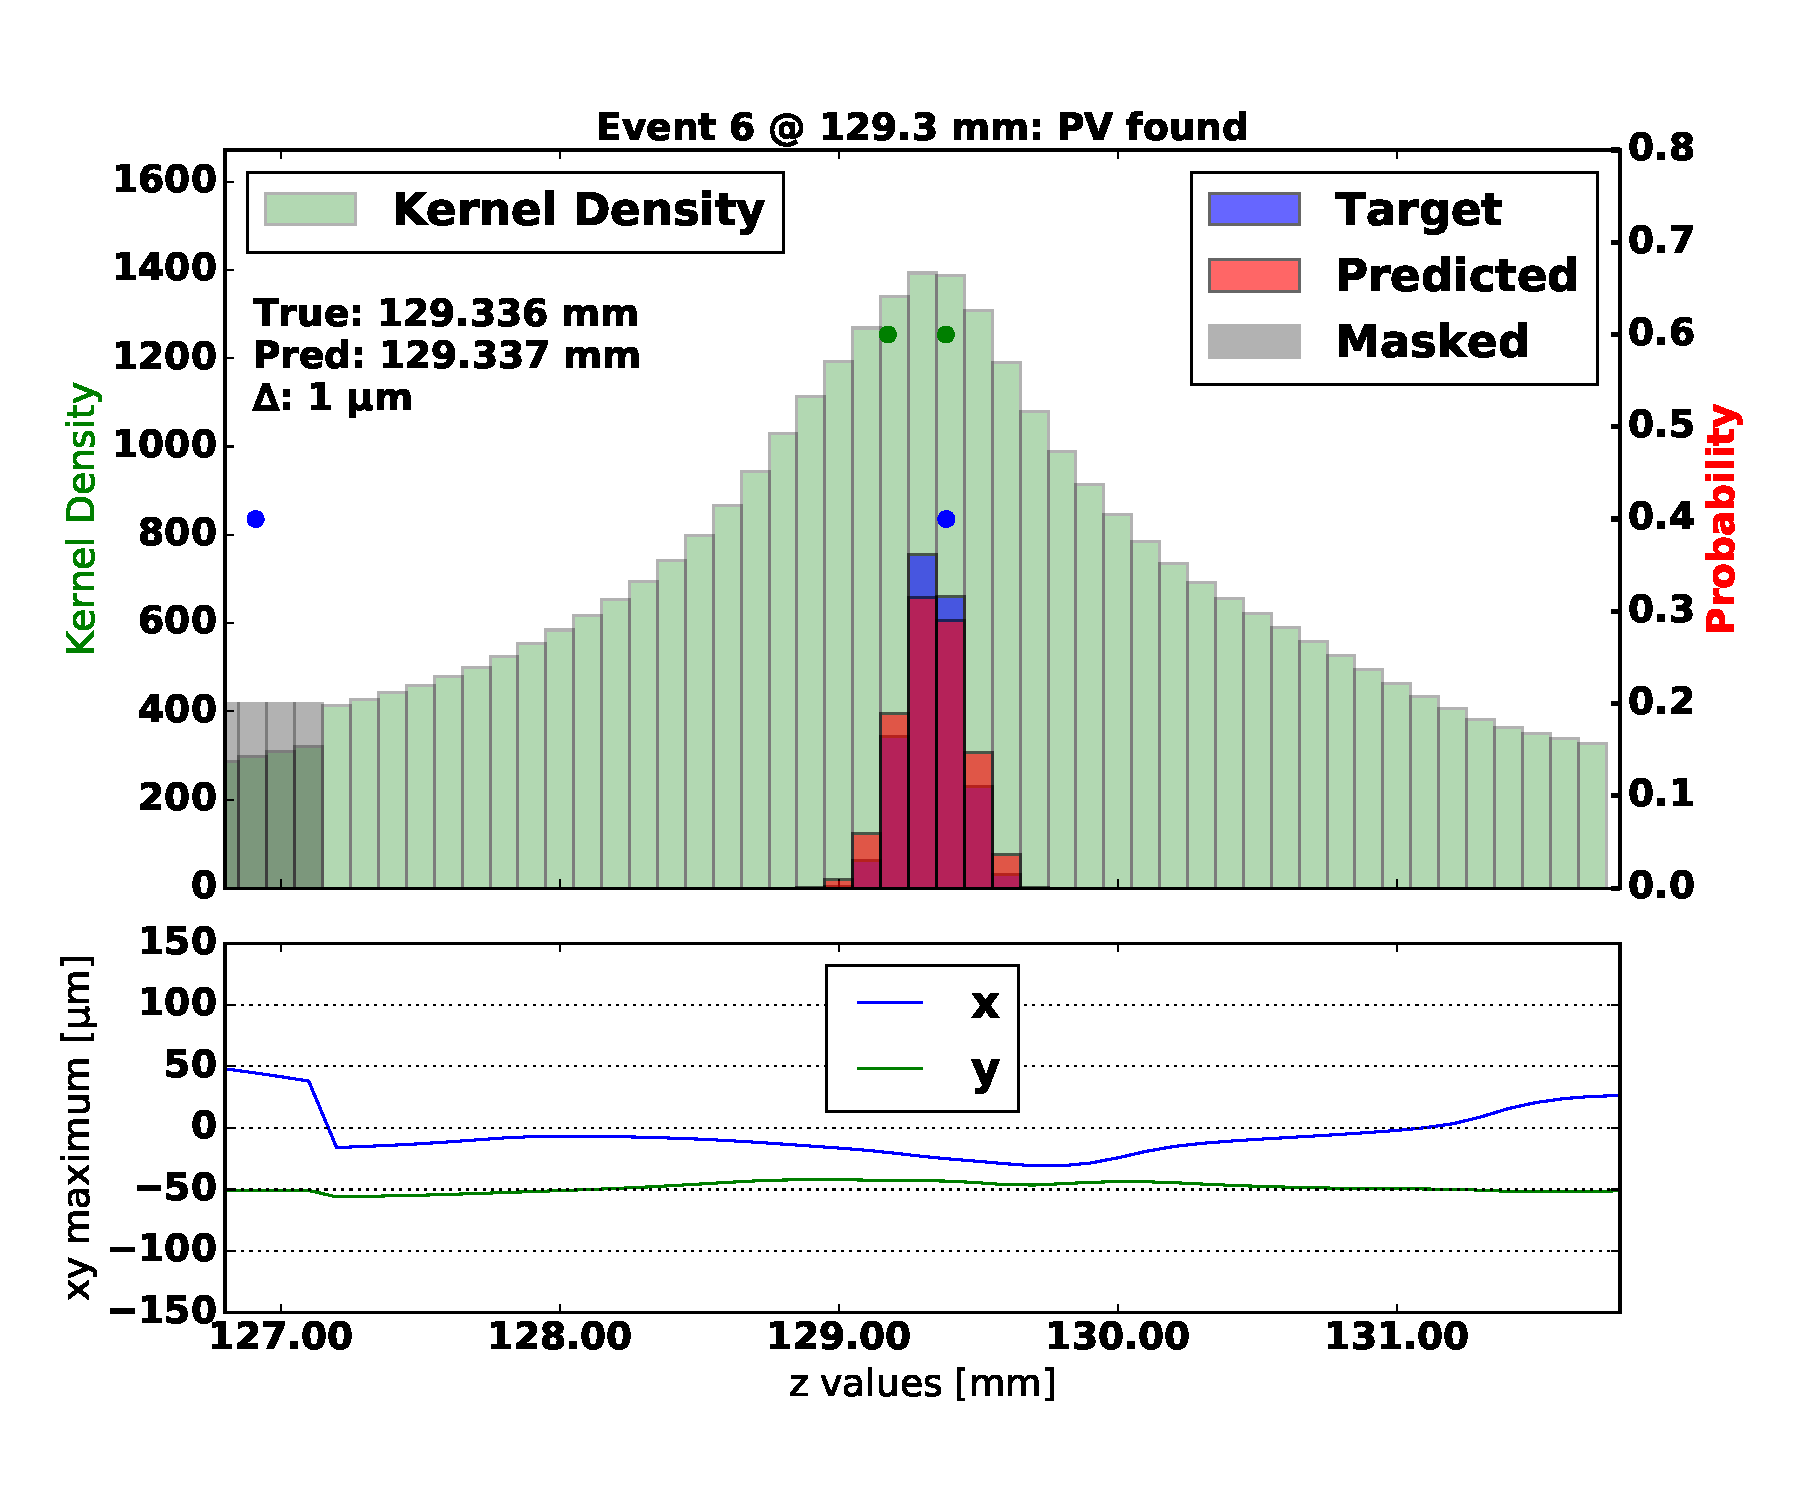
\includegraphics[width=1\textwidth, trim=60 0 60 0]{images/07Jan19_AltCNN4Layer_D35_sp_33.pdf}
        \end{center}
    \column{.5\textwidth}
        \begin{center}
           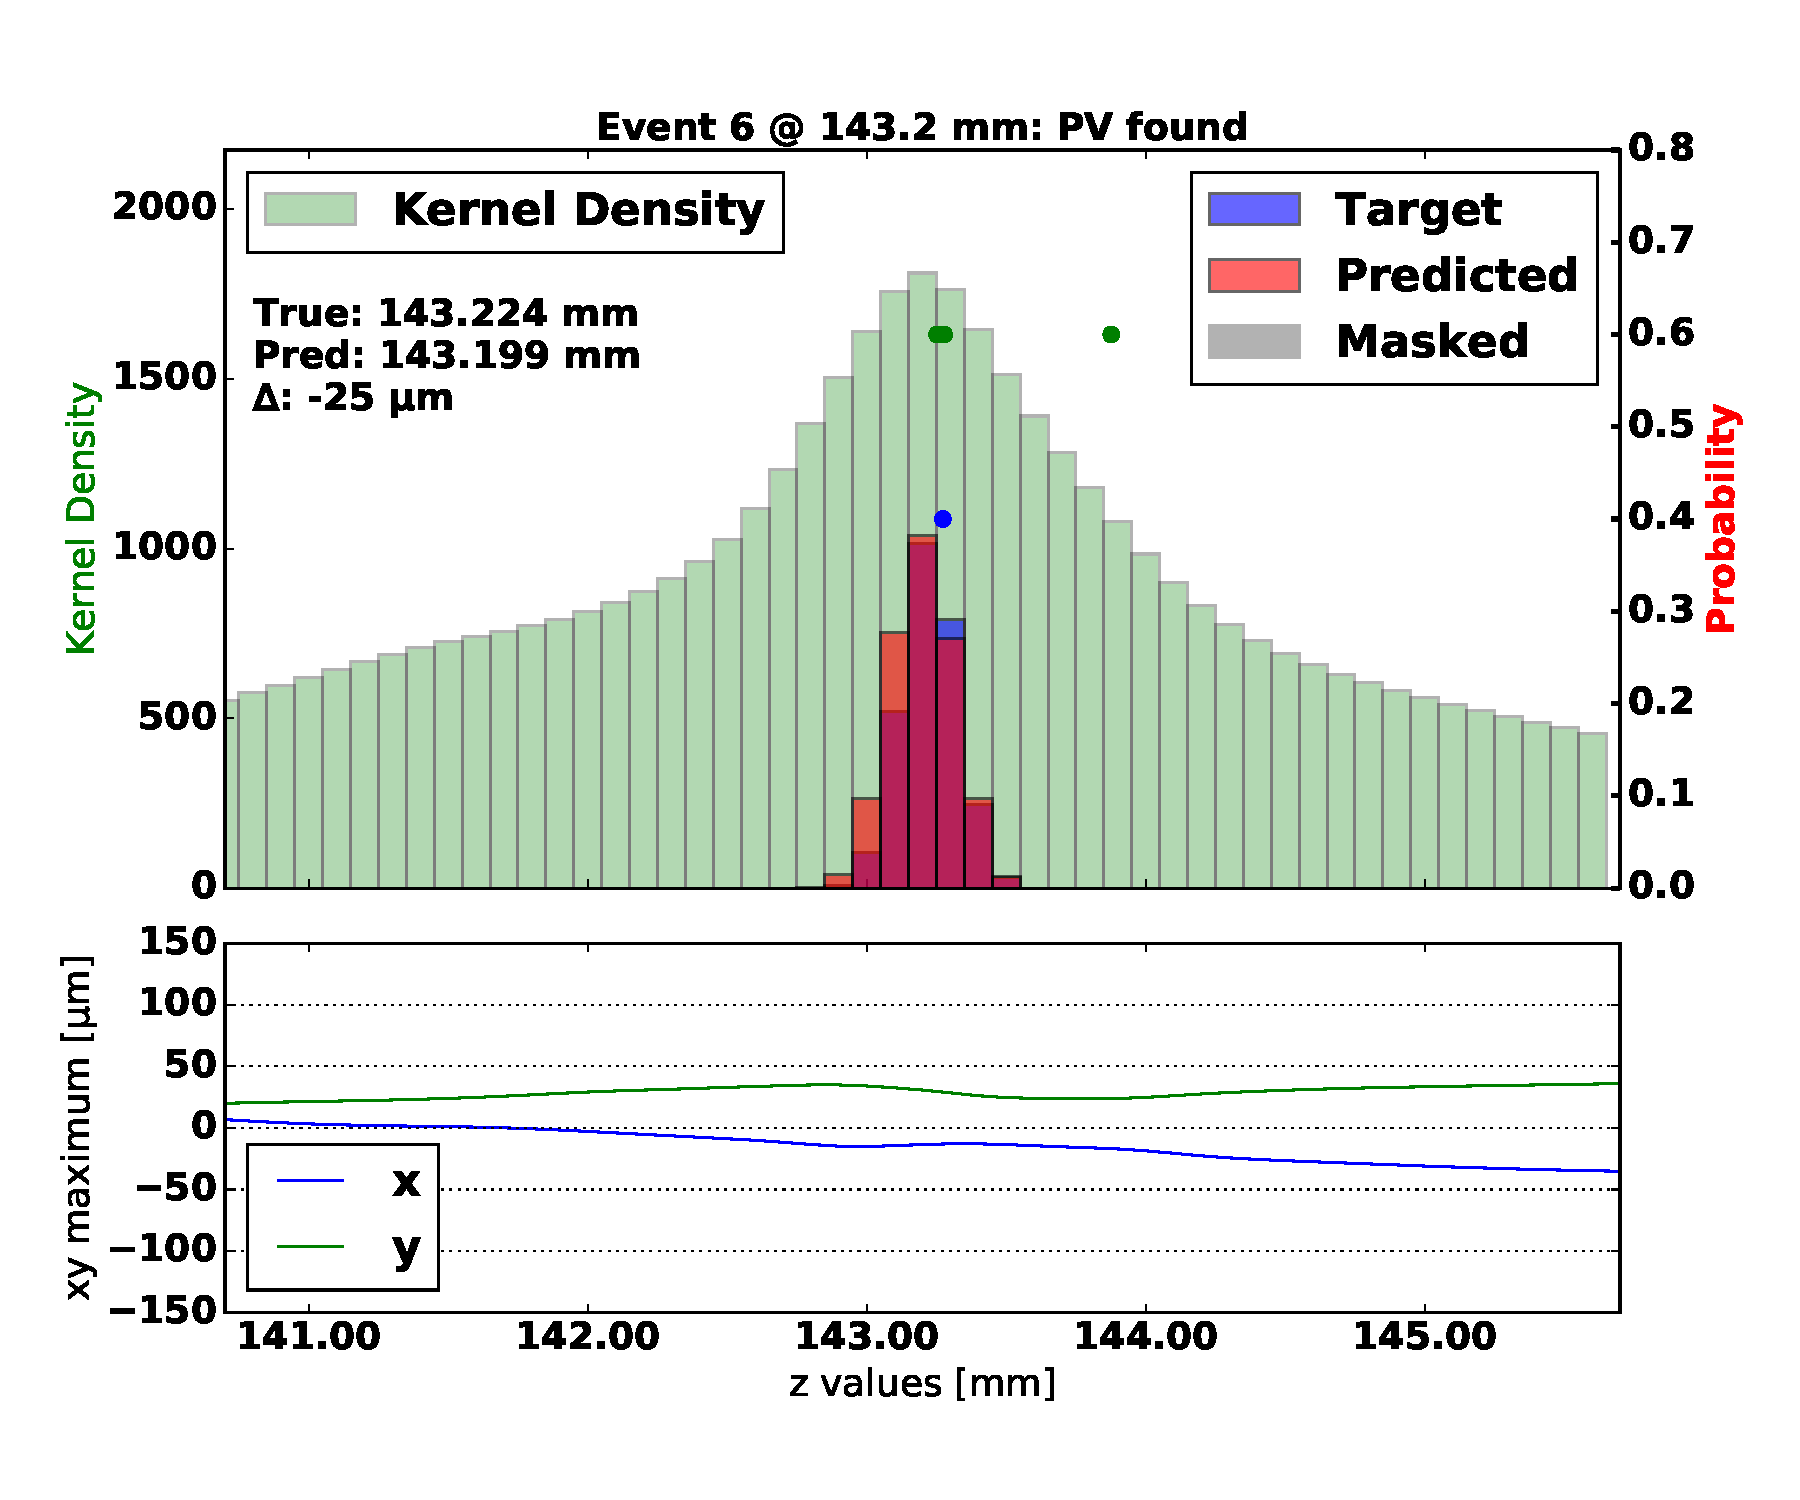
\includegraphics[width=1\textwidth, trim=60 0 60 0]{images/07Jan19_AltCNN4Layer_D35_sp_34.pdf}
       \end{center}
  \end{columns}
\end{frame}


\begin{frame}{More predictions with targets (4)}
  \begin{columns}[c]
    \column{.5\textwidth}
        \begin{center}
           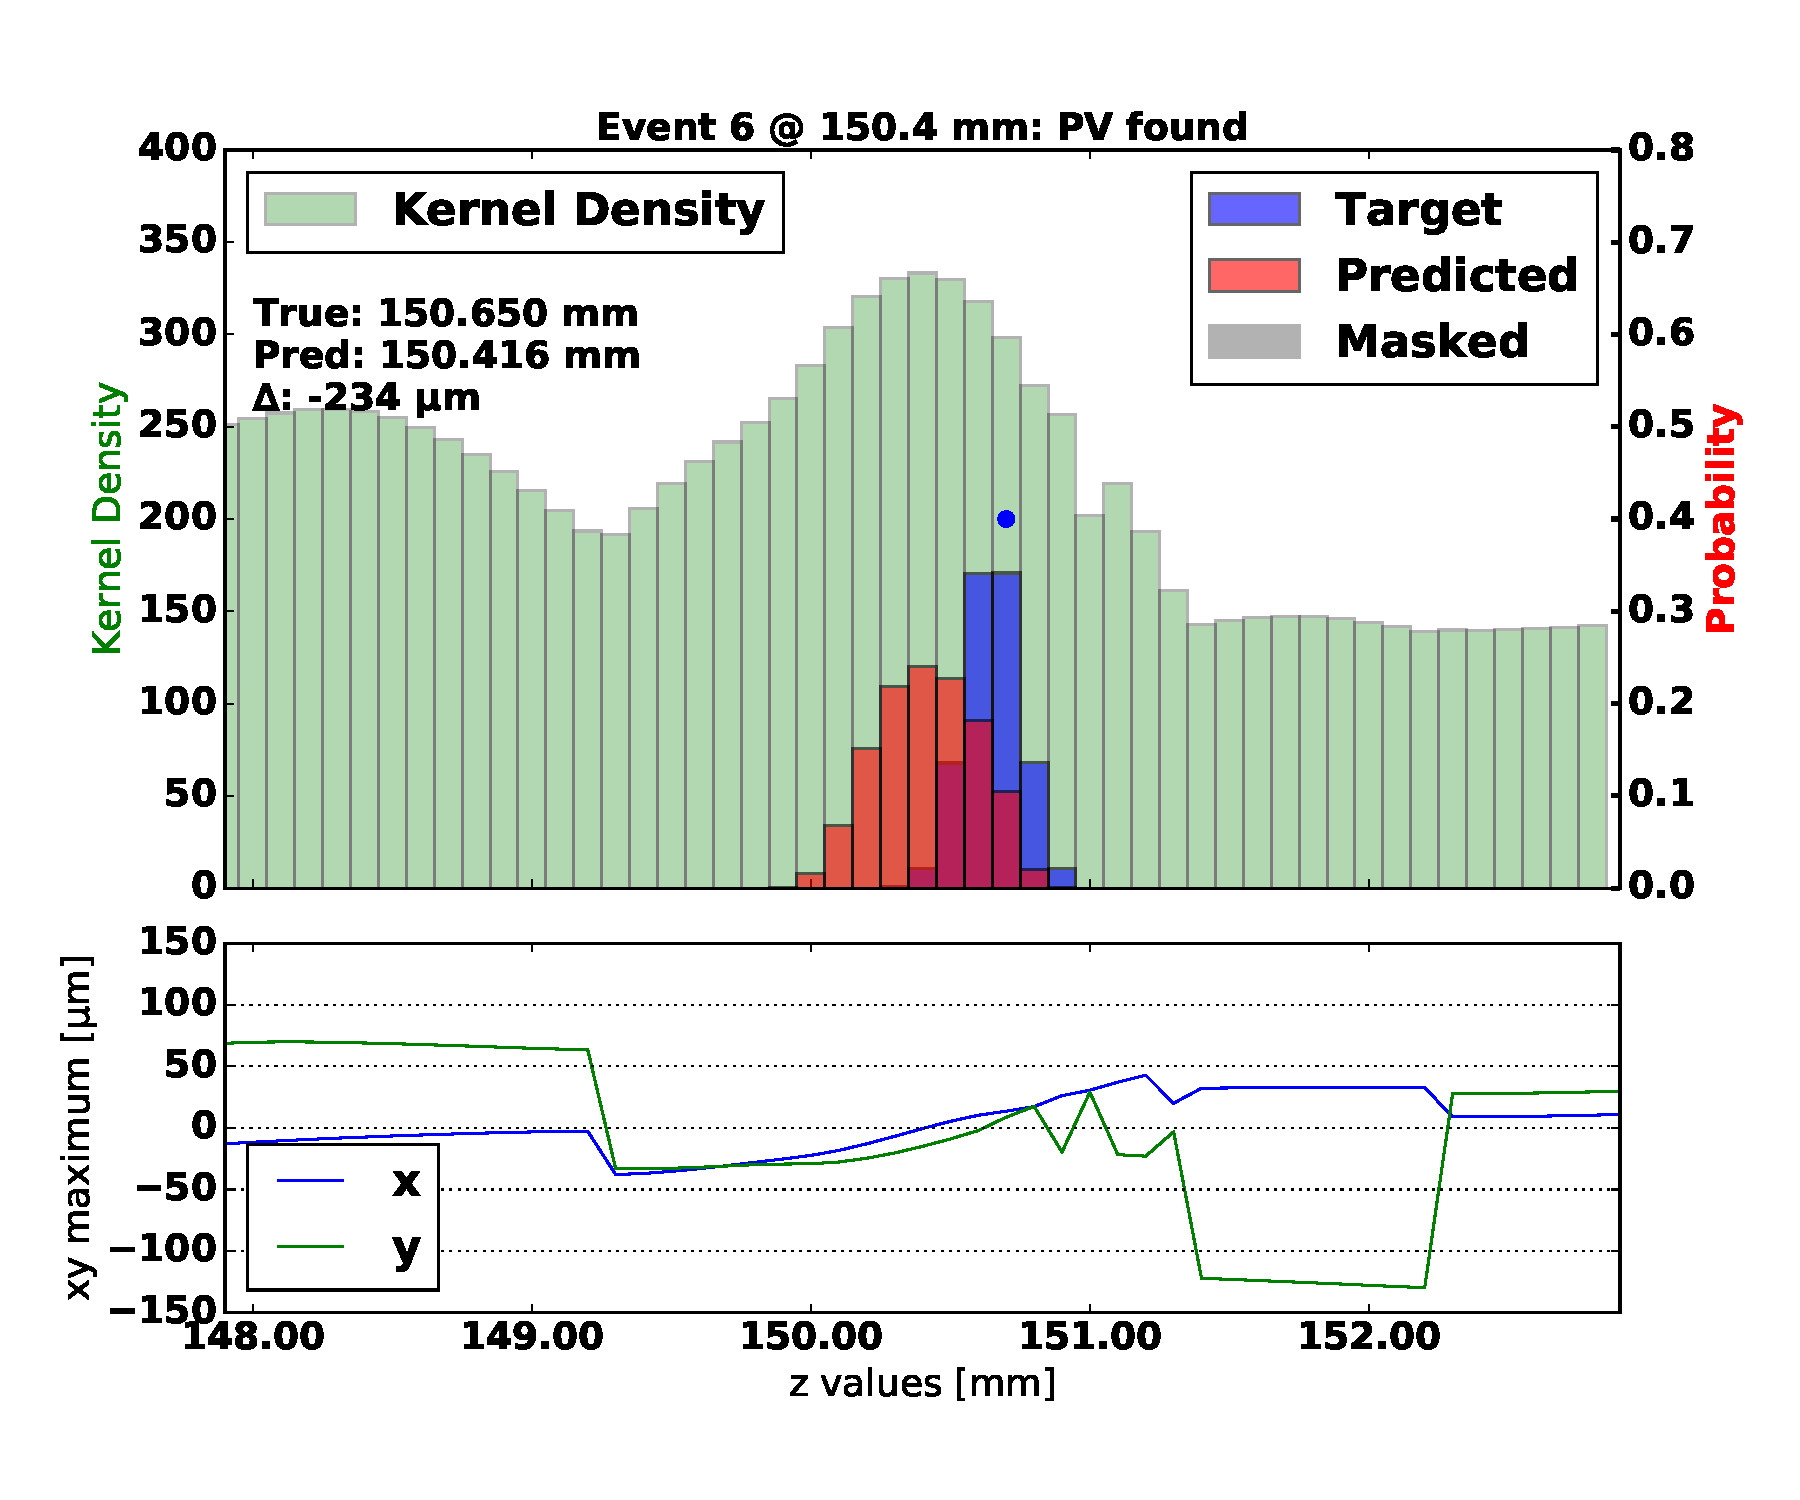
\includegraphics[width=1\textwidth, trim=60 0 60 0]{images/07Jan19_AltCNN4Layer_D35_sp_35.pdf}
        \end{center}
    \column{.5\textwidth}
        \begin{center}
           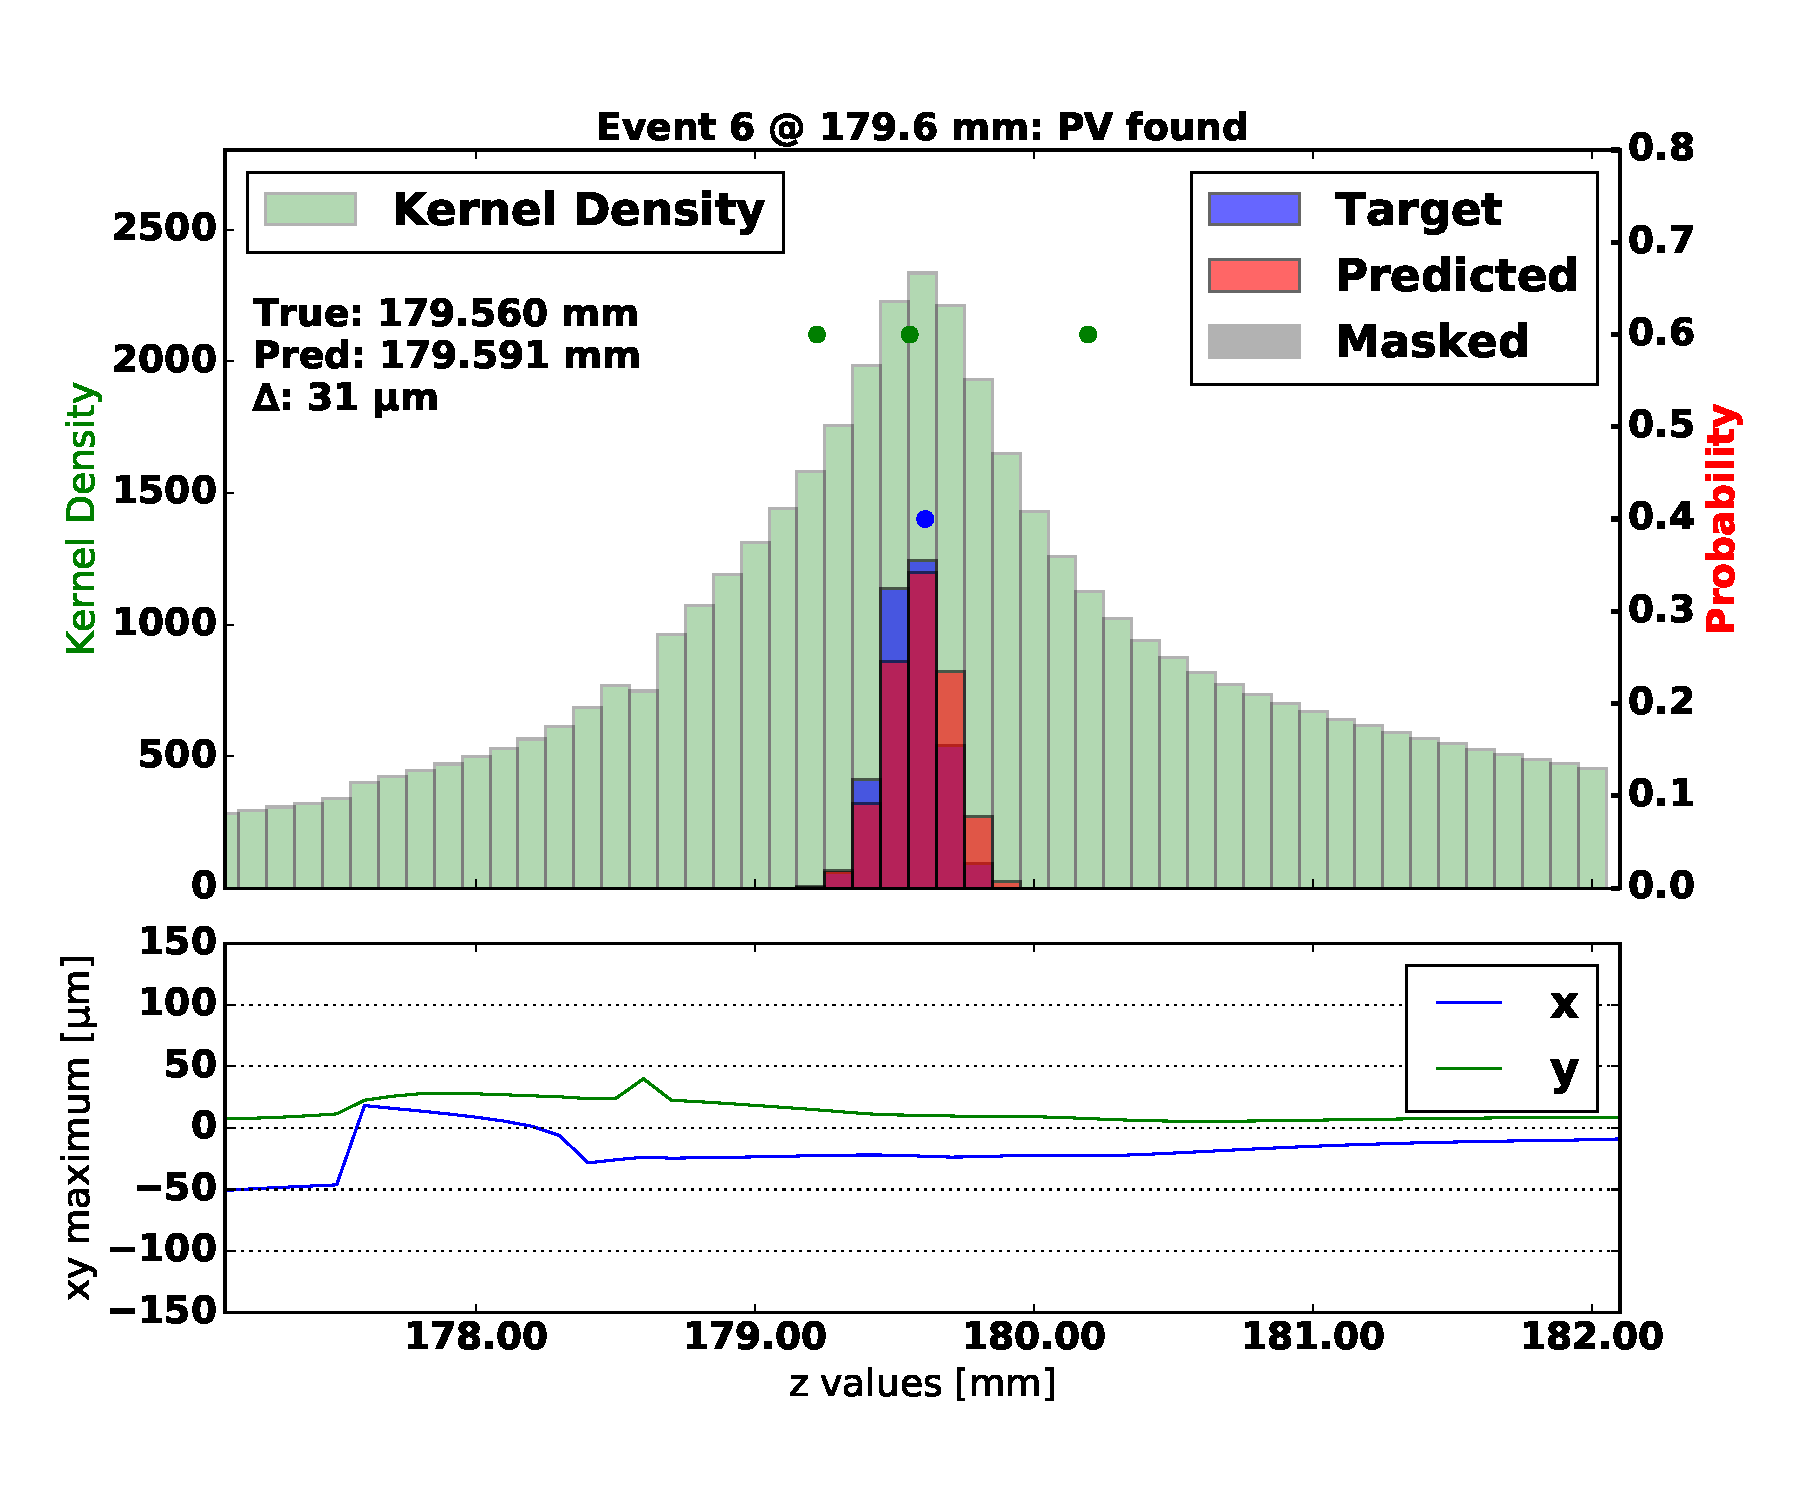
\includegraphics[width=1\textwidth, trim=60 0 60 0]{images/07Jan19_AltCNN4Layer_D35_sp_36.pdf}
       \end{center}
  \end{columns}
\end{frame}


\subsection{The VELO}
\begin{frame}{The VELO}
  \begin{columns}[c]
    \column{.6\textwidth}
    \begin{block}{Tracks}
      \begin{itemize}
          \item Originate from vertices (not shown)
          \item Hits originate from tracks
          \item We only know the true track in simulation
          \item Nearly straight, but tracks may scatter in material
      \end{itemize}
    \end{block}
    \begin{block}{The VELO}
      \begin{itemize}
          \item A set of 26 planes that detect tracks
          \item Tracks should hit one or more pixels per plane
          \item Sparse 3D dataset (41M pixels)
      \end{itemize}
    \end{block}
    \column{.4\textwidth}
    \centering
    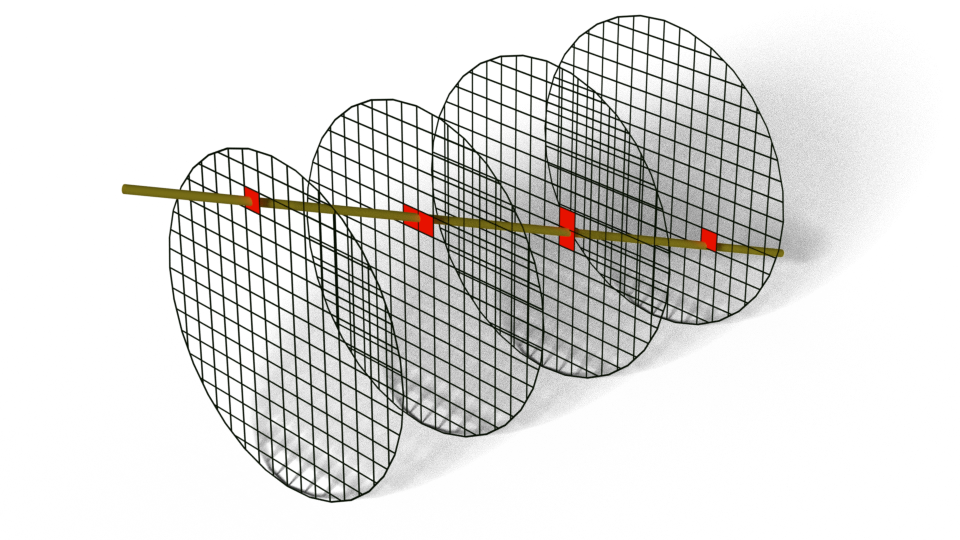
\includegraphics[width=\textwidth, trim=200 0 100 0]{images/Intersections.png}
  \end{columns}
\end{frame}


\subsection{Questions}
\begin{frame}{Questions for other experiments}
    \begin{itemize}
      \item
          Beam width ($x$, $y$): $\unit[40]{\mu m}$ for LHCb, what is yours?
      \item
          Transverse resolution: $\unit[5\textup{--}15]{\mu m}$ for LHCb depending on number of tracks, what is yours?
      \item
          Longitudinal resolution: $\unit[40\textup{--}100]{\mu m}$ for LHCb depending on number of tracks, what is yours?
      \item
          Cleaning up prototracks based on IP could simplify kernel
      \item
          Can prototracking be done in the triggers?
    \end{itemize}
\end{frame}




\backupend


\end{document}
